\documentclass[aspectratio=169,11pt]{beamer}

\usepackage[utf8]{inputenc}
\usepackage[T1]{fontenc}
\usepackage[ngerman]{babel}
\usepackage{graphicx}
\graphicspath{{../}}   % archiviert: Bilder liegen im übergeordneten Ordner images/
\usepackage{booktabs}
\usepackage{array}
\usepackage{amsmath,amssymb,amsfonts}
\usepackage{mathtools}
\usepackage{hyperref}
\usepackage{xcolor}
\usepackage{verbatim}
\usepackage{alltt}

\usetheme{Madrid}
\usecolortheme{default}
\setbeamertemplate{navigation symbols}{}
\setbeamertemplate{footline}[frame number]
\setbeamertemplate{blocks}[rounded][shadow=false]

\setbeamertemplate{headline}{%
  \leavevmode%
  \hbox{%
    \begin{beamercolorbox}[wd=\paperwidth,ht=2.5ex,dp=1.125ex]{subsection in head/foot}%
      \insertsubsectionnavigationhorizontal{\paperwidth}{}{\hskip0pt plus1filll}%
    \end{beamercolorbox}%
  }%
}
\usepackage{listings}
\usepackage{xcolor}

\lstdefinestyle{Rstyle}{
  language=R,
  basicstyle=\ttfamily\small,
  keywordstyle=\color{blue},
  commentstyle=\color{gray}\itshape,
  stringstyle=\color{teal},
  showstringspaces=false,
  extendedchars=true,
  literate={~}{{\makebox[0.525em]{$\sim$}}}1            % exactly 1 tt column
           {<-}{{\makebox[1.05em]{$\leftarrow$}}}2        % exactly 2 tt columns
           {ä}{{\"a}}1 {ö}{{\"o}}1 {ü}{{\"u}}1
           {Ä}{{\"A}}1 {Ö}{{\"O}}1 {Ü}{{\"U}}1
           {ß}{{\ss}}1 {–}{{--}}1 {’}{{'}}1
           {²}{{$^2$}}1,
  upquote=true,
  columns=fullflexible,
  keepspaces=true   % keep source spacing: space after <-/~, aligned comments and R output
}
\lstset{style=Rstyle}

\AtBeginSection[]{%
  \begin{frame}{Überblick}
    \tableofcontents[currentsection,sectionstyle=show/shaded,subsectionstyle=show/show/hide]
  \end{frame}
}

\title{Statistik für Ökonomen}
\subtitle{Teil 3: Regression}
\author{Prof.\ Dr.\ Christoph Weisser}
\institute{HSBI}
\date{}

\begin{document}

% Slide 1: Title Slide
\frame{\titlepage}

% Slide 2: Themen der Veranstaltung
\begin{frame}{Themen der Veranstaltung (1/2)}
  \renewcommand{\arraystretch}{1.1}
  \begin{tabular}{@{}l l@{}}
    \toprule
    \textbf{Teil} & \textbf{Inhalt} \\
    \midrule
    1 -- Deskriptive Statistik & Grundbegriffe, Skalenniveaus, Häufigkeiten, \\
      & Lage- und Streuungsmaße \\
    \addlinespace
    2 -- Grafische Darstellungen & Grafische Darstellungen \\
    \addlinespace
    3 -- Regression & Regression \\
    \addlinespace
    4 -- Wahrscheinlichkeitsrechnung & Grundlagen, Kombinatorik, \\
      & Wahrscheinlichkeitsbegriffe, \\
      & Kolmogorovsche Axiome, \\
      & Bedingte Wahrscheinlichkeiten, \\
      & Satz von Bayes \\
    \bottomrule
  \end{tabular}
\end{frame}

\begin{frame}{Themen der Veranstaltung (2/2)}
  \renewcommand{\arraystretch}{1.1}
  \begin{tabular}{@{}l l@{}}
    \toprule
    \textbf{Teil} & \textbf{Inhalt} \\
    \midrule
    5 -- Wahrscheinlichkeitsverteilungen & Diskrete Verteilungen, \\
      & Stetige Verteilungen, \\
      & Normalverteilung, \\
      & Grenzwertsätze \\
    \addlinespace
    6 -- Induktive Statistik & Schätzverfahren, \\
      & Konfidenzintervalle, \\
      & Hypothesentests \\
    \bottomrule
  \end{tabular}
\end{frame}




\begin{frame}{Symbolverzeichnis (1)}
  \begin{center}
    \renewcommand{\arraystretch}{1.15}
    \begin{tabular}{cl@{\hspace{1em}}cl}
      \toprule
      \textbf{Symbol} & \textbf{Bedeutung} & \textbf{Symbol} & \textbf{Bedeutung} \\
      \midrule
      $\omega$ & Statistische Einheit & $h_j$ & Absolute Häufigkeit \\
      $n$ & Anzahl der statistischen Einheiten & $f_j$ & Relative Häufigkeit \\
      $X$ & Merkmal & $H_j$ & Kumulierte absolute Häufigkeit \\
      $x$ & Merkmalsausprägung & $F(x)$ & Empirische Verteilungsfunktion \\
      $x_i$ & Merkmalswert (beobachteter Wert) & $a_j$ & Merkmalsausprägung (Klasse $j$) \\
      $x_{(i)}$ & $i$-ter Wert der geordneten Stichprobe & $\tilde{x}$ & Median \\
      $\bar{x}$ & Arithmetisches Mittel & $\bar{x}_{\text{geo}}$ & Geometrisches Mittel \\
      $\bar{x}_{\text{harm}}$ & Harmonisches Mittel & & \\
      \bottomrule
    \end{tabular}
  \end{center}
\end{frame}

\begin{frame}{Symbolverzeichnis (2)}
  \begin{center}
    \renewcommand{\arraystretch}{1.15}
    \begin{tabular}{cl@{\hspace{1.2em}}cl}
      \toprule
      \textbf{Symbol} & \textbf{Bedeutung} & \textbf{Symbol} & \textbf{Bedeutung} \\
      \midrule
      $s^2$ & Varianz (Stichprobe) & $s_{xy}$ & Kovarianz von $X$ und $Y$ \\
      $s$ & Standardabweichung & $r$ & Korrelationskoeffizient (Bravais-Pearson) \\
      $R$ & Spannweite & $\beta_0,\,\beta_1$ & Regressionskoeffizienten (wahr) \\
      $\text{IQR}$ & Interquartilsabstand & $\hat{\beta}_0,\,\hat{\beta}_1$ & Geschätzte Regressionskoeffizienten \\
      $x_{0{,}25},\,x_{0{,}75}$ & 25\,\%- und 75\,\%-Quantil & $y_i$ & Beobachtete $y$-Werte \\
      $Q_1,\,Q_3$ & 1. und 3. Quartil & $\hat{y}_i$ & Geschätzte $y$-Werte \\
      & & $u_i$ & Störterm (Fehler) \\
      & & $\hat{u}_i$ & Residuum \\
      & & $R^2$ & Bestimmtheitsmaß \\
      \bottomrule
    \end{tabular}
  \end{center}
\end{frame}


% ===== SECTION: GRUNDLAGEN =====
% ===== SUBSECTION: GRAFISCHE DARSTELLUNGEN =====

% ===== SECTION: REGRESSION =====
\section{Regression}

% Slide 105: Regression Intro

% ---- Slide 1: Zusammenhang metrischer Merkmale -------------
\begin{frame}{Zusammenhang zweier metrischer Merkmale}
  \begin{block}{Fragestellung}
    Untersucht werden soll der Zusammenhang zwischen zwei metrisch
    skalierten Merkmalen.
  \end{block}

  \medskip

  \begin{itemize}
    \item \textbf{Exogene Variable $X$:} von außen gegeben, unabhängig
          angenommen -- auch \emph{erklärende Variable}.
    \item \textbf{Endogene Variable $Y$:} abhängiges Merkmal -- auch
          \emph{zu erklärende Variable}.
  \end{itemize}
\end{frame}


% ---- Slide 2: Zuordnung und Begründung ---------------------



% ---- Slide 1: Regression -- ein Beispiel -------------------
\begin{frame}{Regression -- ein Beispiel}
  \begin{block}{Szenario}
    Eine neue Leuchte wird zum Test in mehreren Geschäften zu
    unterschiedlichen Preisen angeboten. Beobachtet werden Preis
    (in Euro) und Absatzmenge.
  \end{block}

  \medskip

  \begin{center}
    \begin{tabular}{l*{9}{r}}
      \toprule
      Preis $x_i$ (Euro)  & 80 & 85 & 90 & 95 & 100 & 105 & 110 & 115 & 120 \\
      \midrule
      Menge $y_i$         & 20 & 17 & 15 & 9  & 11  & 8   & 4   & 4   & 2   \\
      \bottomrule
    \end{tabular}
  \end{center}

  \medskip

  \begin{exampleblock}{Zuordnung der Variablen}
    Der Preis war in jedem Geschäft fest vorgegeben und nicht verhandelbar.
    Daher ist
    \begin{itemize}
      \item der \textbf{Preis} das \emph{exogene} Merkmal $X$,
      \item die \textbf{Menge} das \emph{endogene} Merkmal $Y$
            (Ergebnis des Kaufverhaltens, abhängig vom Preis).
    \end{itemize}
  \end{exampleblock}
\end{frame}


% ---- Slide 2: Preis-Absatz- vs. Nachfragefunktion ----------
\begin{frame}{Preis-Absatz- und Nachfragefunktion}
  \begin{block}{Preis-Absatzfunktion}
    Der gesuchte funktionale Zusammenhang $Y = f(X)$ heißt
    \emph{Preis-Absatzfunktion}. Sie beantwortet die Frage:
    \emph{Welche Menge wird zu einem vorgegebenen Preis abgesetzt?}
  \end{block}

  \medskip

  \begin{block}{Nachfragefunktion}
    Die Umkehrfunktion $X = f^{-1}(Y)$ heißt \emph{Nachfragefunktion}.
    Sie beantwortet die umgekehrte Frage: \emph{Zu welchem Preis kann
    eine festgelegte Menge verkauft werden?}
  \end{block}

  \end{frame}

% Slide 107: Regression Beispiel 2
\begin{frame}{Regression -- Beispiel (Warnung)}
  \begin{center}
    \begin{tabular}{lrrrrrrrrr}
      \toprule
      Preis $x_i$ (Euro) & 80 & 85 & 90 & 95 & 100 & 105 & 110 & 115 & 120 \\
      \midrule
      Absatz $y_i$       & 20 & 17 & 15 & 12 & 10  & 8   & 6   & 4   & 2   \\
      \bottomrule
    \end{tabular}
  \end{center}

  \medskip

  \begin{alertblock}{Warnung}
    \begin{itemize}
      \item \textbf{Nicht sortieren!}\\
            Die Werte $x_i$ und $y_i$ dürfen \emph{nicht} unabhängig
            voneinander umsortiert werden.
      \item \textbf{Paare gehören zusammen.}\\
            Jedes Paar $(x_i, y_i)$ stammt aus \emph{derselben Beobachtung}
            (hier: aus demselben Geschäft) -- die Zuordnung
            Preis $\leftrightarrow$ Absatz darf nicht verloren gehen.
    \end{itemize}
  \end{alertblock}
\end{frame}

% ===== SUBSECTION: STREUUNGSDIAGRAMM =====
\subsection{Streuungsdiagramm}


% Slide 109: Streuungsdiagramm Text
\begin{frame}{Streuungsdiagramm}
  \begin{block}{Idee}
    Ein \emph{Streuungsdiagramm} (auch: \emph{Scatterplot}) verschafft
    einen ersten visuellen Überblick über den Zusammenhang zweier
    metrischer Merkmale $X$ und $Y$.
  \end{block}

  \medskip

  \begin{itemize}
    \item Jede Beobachtung $(x_i, y_i)$ wird als \textbf{ein Punkt}
          eingezeichnet.
    \item Der \textbf{exogene Wert} $x_i$ (hier: Preis) steht auf der
          $x$-Achse.
    \item Der \textbf{endogene Wert} $y_i$ (hier: Absatzmenge) steht auf
          der $y$-Achse.
    \item Aus der Punktewolke lassen sich \emph{Richtung}, \emph{Stärke}
          und \emph{Form} des Zusammenhangs ablesen.
  \end{itemize}
\end{frame}

% Slide 110: Streuungsdiagramm Image 1
\begin{frame}{Streuungsdiagramm}
  \begin{center}
    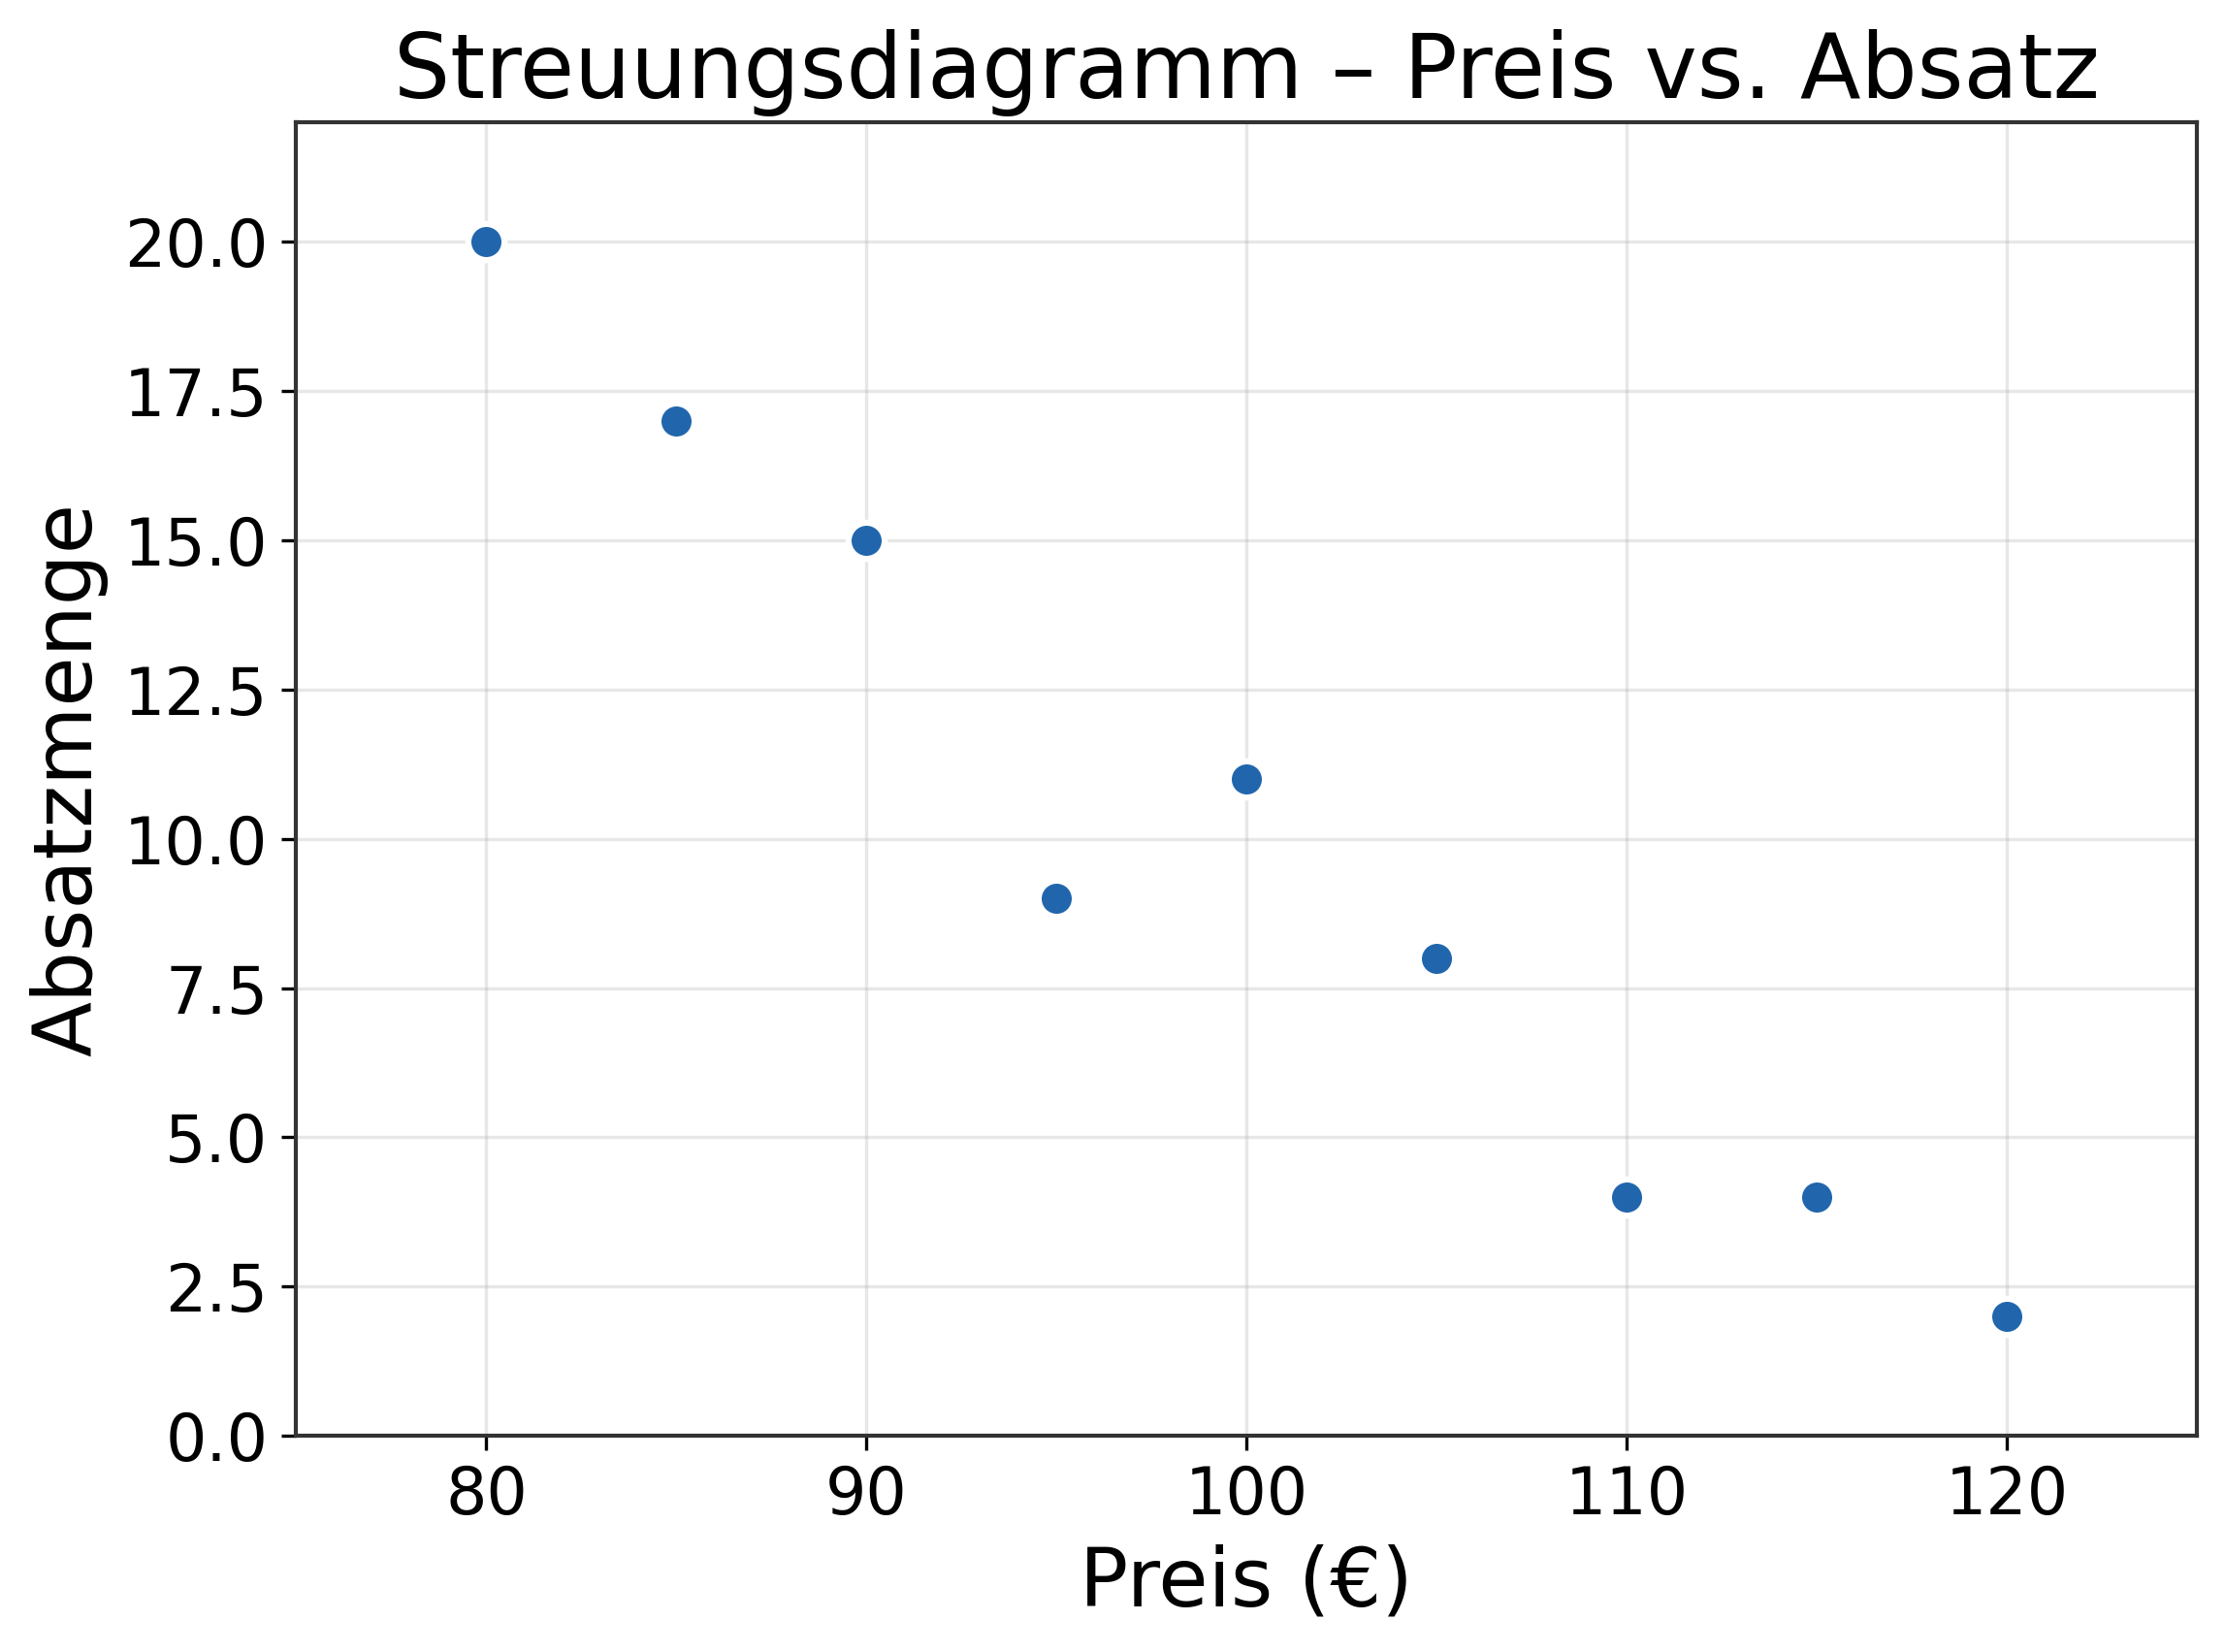
\includegraphics[width=0.8\textwidth,height=0.75\textheight,keepaspectratio]{images/image_020.png}
  \end{center}
\end{frame}

% Slide 111: Streuungsdiagramm Image 2
\begin{frame}{Kovarianz}
  \begin{block}{Idee}
    Die \emph{Kovarianz} $s_{xy}$ misst die \textbf{gemeinsame Variabilität}
    zweier metrischer Merkmale $X$ und $Y$.
  \end{block}

  \begin{block}{Berechnung (Stichprobenkovarianz)}
    \[
      s_{xy} \;=\; \operatorname{Cov}(X, Y)
             \;=\; \frac{1}{n-1} \sum_{i=1}^{n}
                   (x_i - \bar{x})(y_i - \bar{y})
    \]
    mit Wertebereich $\; -\infty < s_{xy} < +\infty$.
  \end{block}
\end{frame}


% Slide 115: Kovarianz - Interpretation
\begin{frame}{Kovarianz -- Interpretation}
  \small
  \begin{block}{Vorzeichen zeigt die Richtung des Zusammenhangs}
    \begin{description}
      \item[$s_{xy} > 0$] \textbf{Positiver (gleichläufiger) Zusammenhang.}\\
            Größere Werte von $X$ gehen tendenziell mit größeren Werten
            von $Y$ einher -- im Streuungsdiagramm eine \emph{positiv
            gerichtete} Punktewolke.
      \item[$s_{xy} < 0$] \textbf{Negativer (gegenläufiger) Zusammenhang.}\\
            Größere Werte von $X$ gehen tendenziell mit kleineren Werten
            von $Y$ einher -- eine \emph{negativ gerichtete} Punktewolke.
      \item[$s_{xy} = 0$] \textbf{Kein linearer Zusammenhang.}\\
            Die gemeinsame Variabilität weist keine Richtung auf;
            die Punktewolke zeigt keine erkennbare lineare Struktur.
    \end{description}
  \end{block}

  \begin{alertblock}{Betrag nicht direkt interpretierbar}
    Die Kovarianz $s_{xy}$ hat die Einheit \glqq Einheit von $X$ $\cdot$
    Einheit von $Y$\grqq{} und hängt von der Skalierung der Daten ab.
  \end{alertblock}
\end{frame}

% Slide 116: Korrelationskoeffizient - Definition
\begin{frame}{Korrelationskoeffizient}
  \begin{block}{Idee}
    Der Korrelationskoeffizient $r_{xy}$ ist eine
    \textbf{normierte Kovarianz}: er misst die Stärke und Richtung des
    \emph{linearen} Zusammenhangs zwischen $X$ und $Y$ -- aber im
    Gegensatz zur Kovarianz \emph{unabhängig von den Maßeinheiten}.
  \end{block}

  \begin{block}{Berechnung}
    \[
      r_{xy} \;=\; \frac{s_{xy}}{s_x \, s_y}
             \;=\; \operatorname{Cov}(X^{*},Y^{*})
             \;=\; \operatorname{Cov}\!\left(
                     \frac{X-\bar{x}}{s_x},\;
                     \frac{Y-\bar{y}}{s_y}
                   \right)
    \]
    mit Wertebereich $\;-1 \le r_{xy} \le +1$.
  \end{block}


  \begin{exampleblock}{Lesart}
    $r_{xy}$ ist die Kovarianz der \emph{z-standardisierten} Variablen
    $X^{*} = (X-\bar{x})/s_x$ und $Y^{*} = (Y-\bar{y})/s_y$. Durch die
    Division durch $s_x s_y$ werden die Einheiten herausgekürzt.
  \end{exampleblock}
\end{frame}

% Slide 117: Korrelationskoeffizient - Interpretation
% ---- Slide 1: Was misst r_xy und wie stark? ----------------
\begin{frame}{Korrelationskoeffizient -- Stärke des Zusammenhangs}
  \begin{block}{Was $r_{xy}$ misst}
    Der Korrelationskoeffizient misst den \textbf{Grad der linearen
    Abhängigkeit} zwischen $X$ und $Y$.
  \end{block}

  \medskip

  \begin{block}{Stärke des Zusammenhangs (Faustregel)}
    \begin{center}
      \renewcommand{\arraystretch}{1.2}
      \begin{tabular}{ll}
        \toprule
        \textbf{Bereich} & \textbf{Interpretation} \\
        \midrule
        $|r_{xy}| > 0{,}8$               & starke Korrelation \\
        $0{,}5 \le |r_{xy}| \le 0{,}8$   & mittlere Korrelation \\
        $|r_{xy}| < 0{,}5$               & schwache Korrelation \\
        \bottomrule
      \end{tabular}
    \end{center}
  \end{block}
\end{frame}


% ---- Slide 2: Grenzen des Korrelationskoeffizienten --------
\begin{frame}{Korrelationskoeffizient -- Grenzen}
  \begin{alertblock}{Kein Erklärungszusammenhang}
    Aus $r_{xy}$ allein lässt sich \emph{nicht} ableiten, welches
    Merkmal unabhängig ($X$) und welches abhängig ($Y$) ist.
    Die Korrelation ist \textbf{symmetrisch}: $r_{xy} = r_{yx}$.
  \end{alertblock}

  \medskip

  \begin{alertblock}{Scheinkorrelation möglich}
    $r_{xy}$ kann $\ne 0$ sein, \textbf{ohne} dass ein inhaltlicher
    Zusammenhang zwischen $X$ und $Y$ besteht -- z.\,B.\ wenn beide
    Variablen durch eine gemeinsame Drittvariable beeinflusst werden.
  \end{alertblock}

  \medskip

  \begin{block}{Merke}
    Ein hoher Wert von $|r_{xy}|$ ist ein \emph{statistischer Befund},
    keine \emph{kausale Aussage}. 
  \end{block}
\end{frame}



% Slide 119: Kovarianz/Korrelation mit R
\begin{frame}[fragile]{Kovarianz und Korrelation mit R}
\begin{lstlisting}
# Kovarianz
cov(x, y)

# Korrelationskoeffizient
cor(x, y)

# Nach Pearson (Standard)
cor(x, y, method = "pearson")
\end{lstlisting}
\end{frame}



% ===== SUBSECTION: KLEINSTE-QUADRATE-SCHÄTZUNG =====
\subsection{Kleinste-Quadrate-Schätzung}

\begin{frame}{Kleinste-Quadrate-Schätzung}
  Kleinste-Quadrate-Schätzung -- Bestimmung der besten Geraden
\end{frame}

% Slide 122: Motivation
\begin{frame}{Motivation}
  Wie kann man die beste Gerade durch die Punktewolke bestimmen?
\end{frame}

\begin{frame}{Die beste Gerade durch die Punktewolke}
  \begin{block}{Regressionsgleichung}
    Der gesuchte lineare Zusammenhang zwischen $X$ und $Y$ wird durch
    eine Gerade beschrieben:
    \begin{center}
      $y_i \;=\; \beta_0 + \beta_1 \, x_i$
    \end{center}
    \begin{description}
      \item[$\beta_0$] \emph{Achsenabschnitt} -- Wert von $y$ bei $x=0$;
            ohne $\beta_0$ gingen alle Geraden durch den Ursprung.
      \item[$\beta_1$] \emph{Steigung} -- Änderung von $y$, wenn $x$ um
            eine Einheit steigt.
    \end{description}
  \end{block}

  \begin{exampleblock}{Schätzung und Bezeichnung}
    Die Koeffizienten $\beta_0$ und $\beta_1$ werden aus den Daten
    über eine Formel \textbf{geschätzt}. Da sie nur in der Potenz~$1$
    auftreten, spricht man von einer \textbf{linearen Regression}.
  \end{exampleblock}
\end{frame}

\begin{frame}{Schätzung der Parameter $\beta_0,\beta_1$}
  \begin{block}{Ziel}
    $Y$ soll möglichst gut durch die lineare
    Funktion $\beta_0 + \beta_1 X$ beschrieben werden.
  \end{block}

  \begin{block}{Regressionsmodell mit Residuen}
    Da die Beobachtungen die Gerade in der Regel nicht exakt treffen,
    treten \emph{Abweichungen} auf:
    \begin{center}
      $y_i \;=\; \beta_0 + \beta_1 \, x_i + u_i$
    \end{center}
    \begin{description}
      \item[$\beta_0 + \beta_1 x_i$] \emph{systematischer Teil} --
            der durch $X$ erklärte Anteil von $Y$.
      \item[$u_i$] \emph{Residuum} -- der nicht durch $X$ erklärte
            Rest der $i$-ten Beobachtung.
    \end{description}
  \end{block}

  \begin{alertblock}{Anforderung an die Residuen}
    Die Residuen $u_i$ sollen \textbf{keine systematische Information}
    über $Y$ mehr enthalten -- alles Erklärbare muss bereits im
    linearen Teil $\beta_0 + \beta_1 x_i$ stecken.
  \end{alertblock}
\end{frame}


% Slide 124: OLS Criterion

% ---- Slide 1: Kleinste-Quadrate-Methode --------------------
\begin{frame}{Kleinste-Quadrate-Methode (OLS)}
  \begin{block}{Idee}
    Gesucht ist die Gerade $\hat{y} = \hat{\beta}_0 + \hat{\beta}_1\,x$,
    für die die Punktewolke im Mittel \emph{möglichst nahe} an der
    Geraden liegt. Als Abstandsmaß dient die Summe der
    \emph{quadrierten} Residuen.
  \end{block}

  \begin{block}{Minimierungsproblem}
    \begin{center}
      $\displaystyle
        \min_{\hat{\beta}_0,\,\hat{\beta}_1}
        \;\sum_{i=1}^{n} \hat{u}_i^{\,2}
        \;=\;
        \min_{\hat{\beta}_0,\,\hat{\beta}_1}
        \;\sum_{i=1}^{n}
        \bigl(y_i - \hat{\beta}_0 - \hat{\beta}_1 x_i\bigr)^{2}
      $
    \end{center}
    mit den Residuen
    $\hat{u}_i = y_i - \hat{y}_i = y_i - \hat{\beta}_0 - \hat{\beta}_1 x_i$.
  \end{block}

  \begin{exampleblock}{Warum quadrieren?}
    \begin{itemize}
      \item Positive und negative Abweichungen heben sich \emph{nicht} gegenseitig auf.
      \item Große Abweichungen werden stärker bestraft als kleine.
    \end{itemize}
  \end{exampleblock}
\end{frame}

\begin{frame}{Kleinste-Quadrate-Methode}
  \begin{block}{Idee}
    Minimierung der Summe der quadrierten Residuen -- also der
    quadrierten Abstände der Punkte von der Regressionsgeraden.
    Die Lösung erfolgt mithilfe der \textbf{Differentialrechnung}.
  \end{block}

  \begin{block}{Notation}
    Geschätzte Werte werden durch ein \glqq Hütchen\grqq{} gekennzeichnet:
    $\hat{y}_i$, $\hat{\beta}_0$, $\hat{\beta}_1$. Der Achsenabschnitt
    $\hat{\beta}_0$ muss in der Gleichung enthalten sein -- sonst wird
    die Gerade auf Ursprungsgeraden eingeschränkt.
  \end{block}

  \begin{block}{Schätzer}
    \begin{center}
      $\displaystyle
        \hat{\beta}_1 \;=\; \frac{s_{xy}}{s_x^{\,2}}
        \qquad\qquad
        \hat{\beta}_0 \;=\; \bar{y} - \hat{\beta}_1\,\bar{x}
      $
    \end{center}
  \end{block}
\end{frame} 

\begin{frame}{Kleinste-Quadrate-Lösung}
  \begin{block}{Steigung}
    \begin{center}
      $\displaystyle
        \hat{\beta}_1 \;=\; \frac{s_{xy}}{s_x^{\,2}}
      $
    \end{center}
    Der Quotient aus \emph{Kovarianz} von $X$ und $Y$ und \emph{Varianz}
    von $X$.
  \end{block}

  \begin{block}{Achsenabschnitt}
    \begin{center}
      $\displaystyle
        \hat{\beta}_0 \;=\; \bar{y} - \hat{\beta}_1 \, \bar{x}
      $
    \end{center}
    Ergibt sich so, dass die Regressionsgerade durch den
    \emph{Schwerpunkt} $(\bar{x}, \bar{y})$ der Punktewolke verläuft.
  \end{block}
\end{frame}


% ---- Slide 2: Interpretation -------------------------------
\begin{frame}{Kleinste-Quadrate-Lösung -- Interpretation}
  \begin{exampleblock}{Eigenschaften der Steigung $\hat{\beta}_1$}
    \begin{itemize}
      \item $\hat{\beta}_1$ übernimmt das \textbf{Vorzeichen} der
            Kovarianz $s_{xy}$.
      \item Die Steigung ist genau dann $0$, wenn $X$ und $Y$
            \textbf{unkorreliert} sind ($s_{xy} = 0$).
      \item Zusammenhang zum Korrelationskoeffizienten:
            \begin{center}
              $\displaystyle
                \hat{\beta}_1 \;=\; r_{xy} \cdot \frac{s_y}{s_x}
              $
            \end{center}
    \end{itemize}
  \end{exampleblock}

  \begin{block}{Merke}
    Regression, Korrelation und Kovarianz hängen eng zusammen:
    Vorzeichen stimmen überein, der Betrag der
    Steigung unterscheidet sich nur durch das Verhältnis der
    Standard\-abweichungen $s_y / s_x$.
  \end{block}
\end{frame}


% Slide 127: KQ Beispiel mit Bild
\begin{frame}{Kleinste-Quadrate Beispiel -- Grafik}
  \begin{center}
    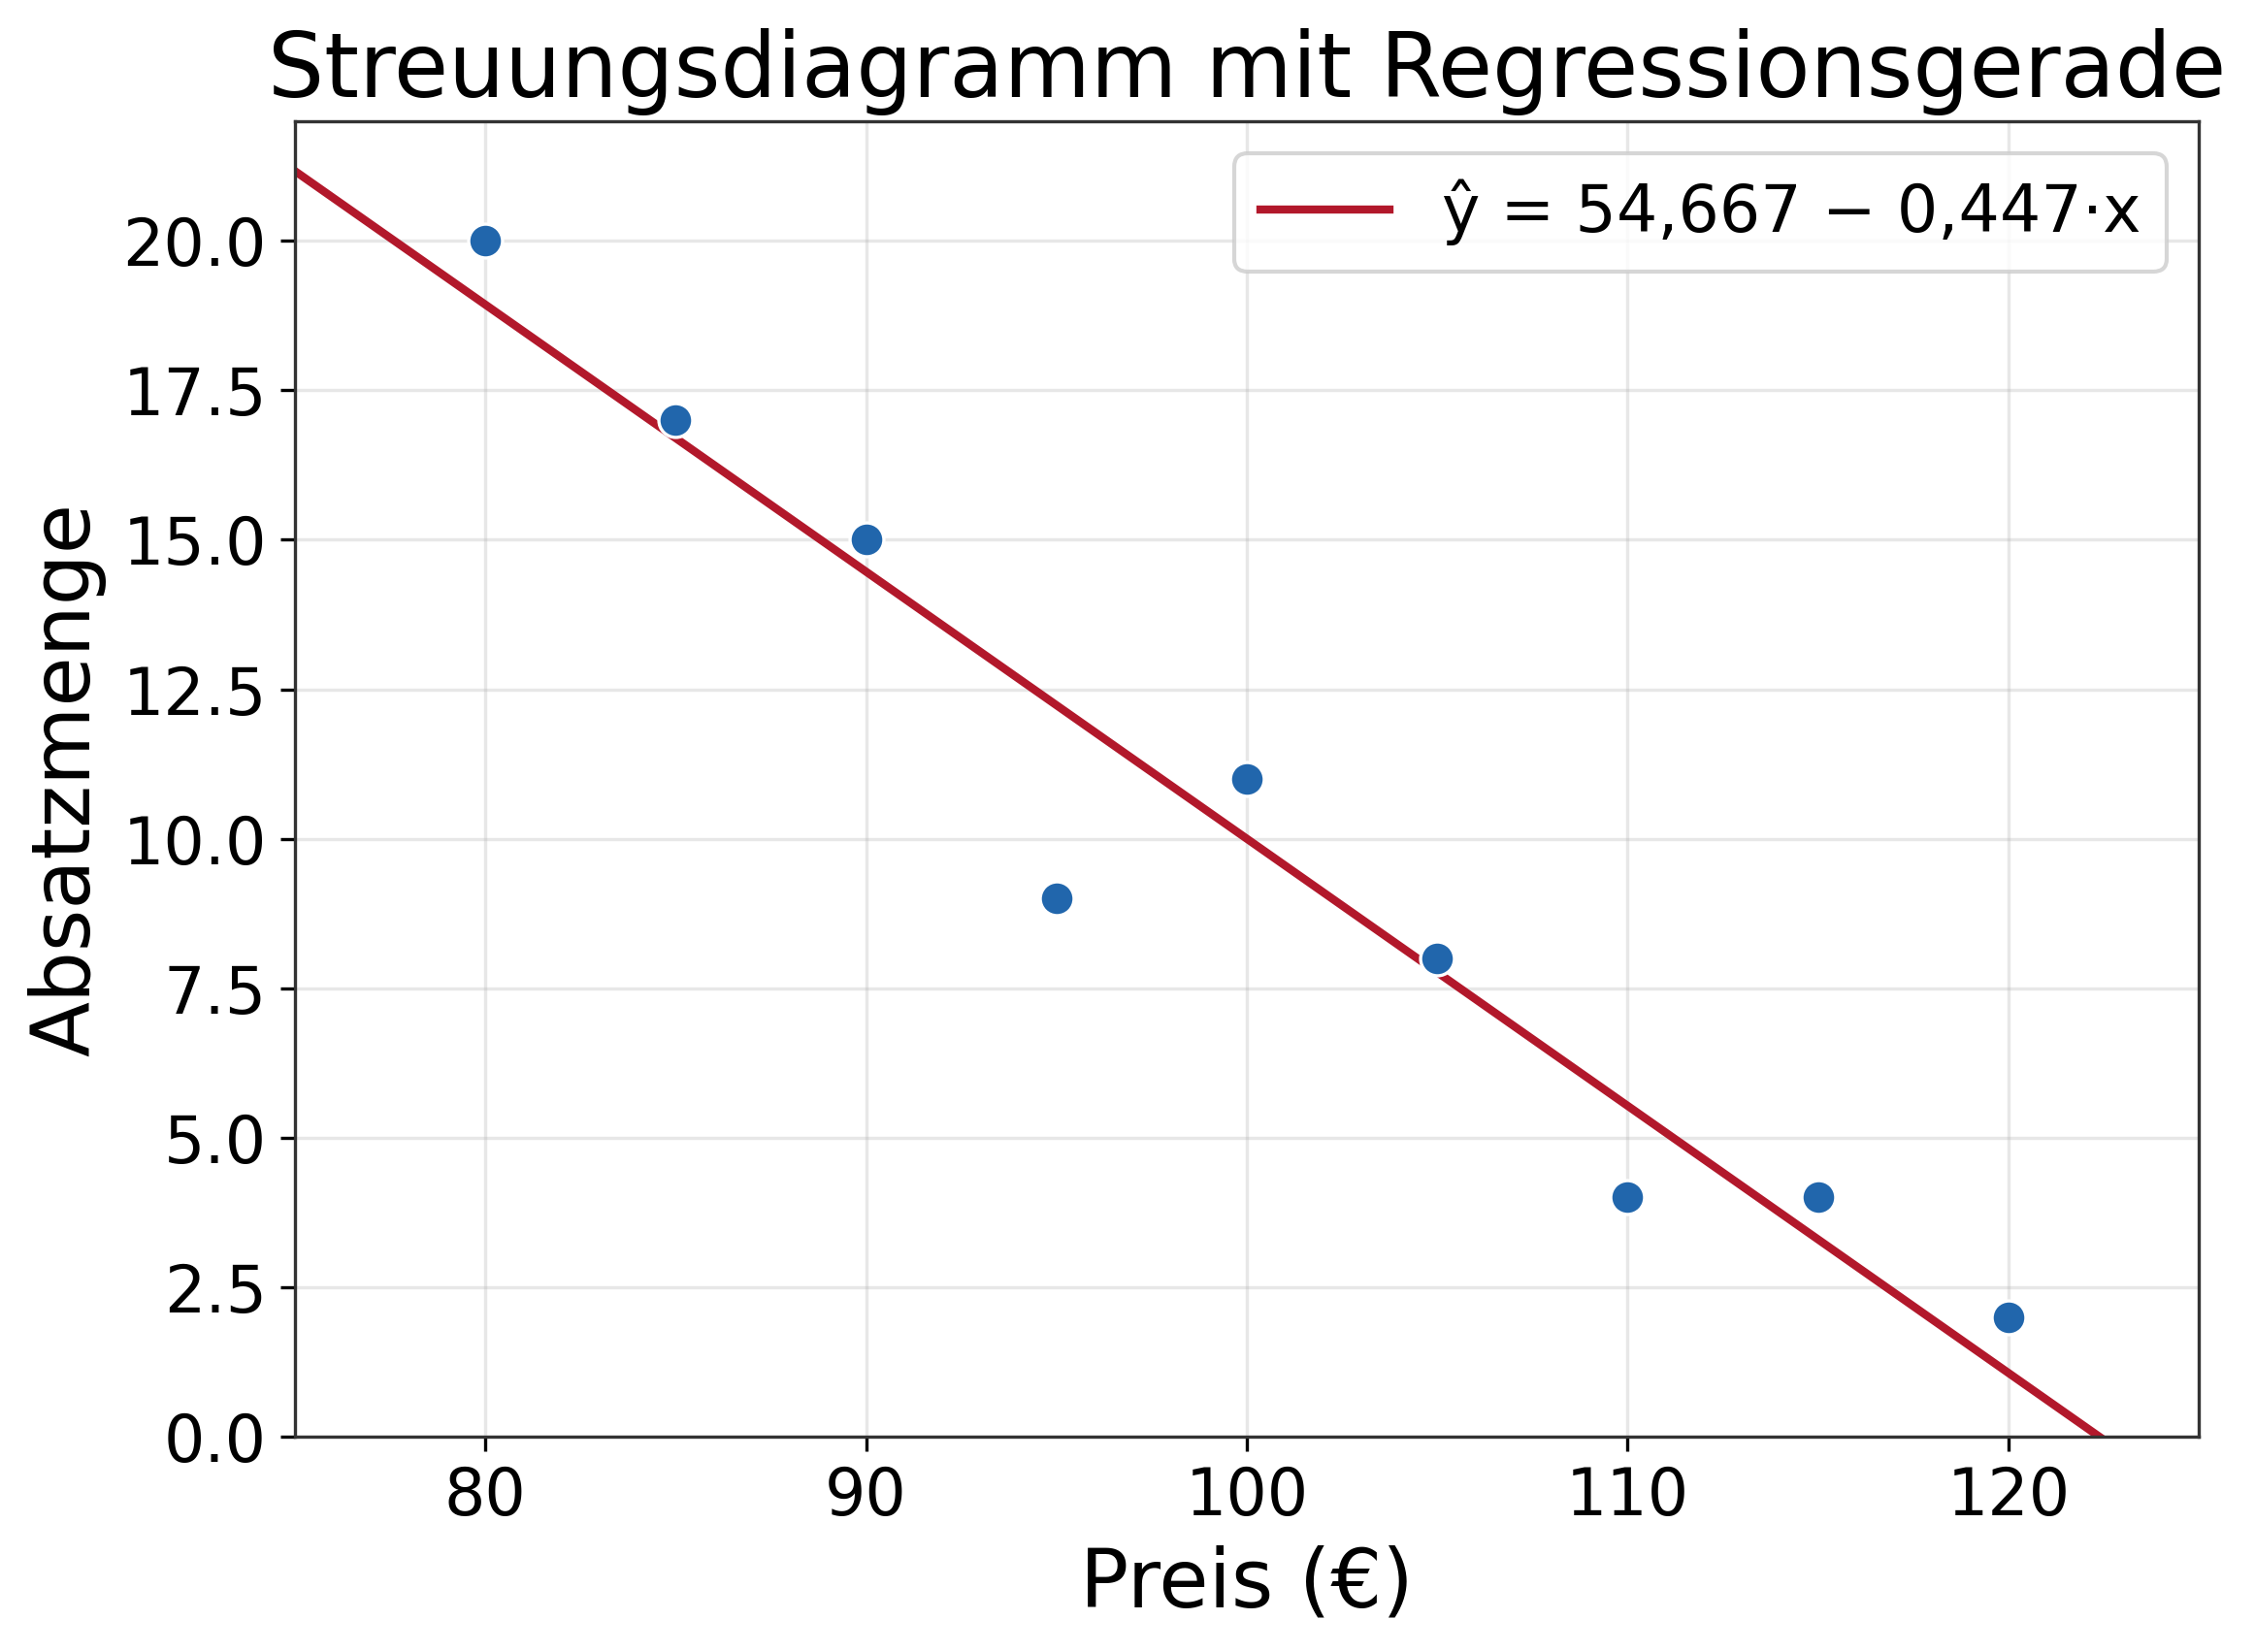
\includegraphics[width=0.8\textwidth,height=0.75\textheight,keepaspectratio]{images/image_021.png}
  \end{center}
\end{frame}

% ---- Slide 1: Regressionsgerade und Steigung ---------------
\begin{frame}{Beispiel: Interpretation der Koeffizienten}
  \begin{block}{Geschätzte Regressionsgerade}
    \begin{center}
      $\displaystyle
        \hat{y}_i \;=\; 54{,}67 \;-\; 0{,}4467 \cdot x_i
      $
    \end{center}
  \end{block}

  \begin{block}{Steigung $\hat{\beta}_1 = -0{,}4467$}
    Steigt der Preis um $1$ Euro, so sinkt die abgesetzte Menge im
    Mittel um $0{,}4467$ Einheiten.
  \end{block}

  \begin{exampleblock}{Ökonomische Lesart}
    Das negative Vorzeichen bestätigt den erwarteten \emph{gegenläufigen}
    Zusammenhang -- eine klassische fallende
    \textbf{Preis-Absatz-Funktion}.
  \end{exampleblock}
\end{frame}


% ---- Slide 2: Achsenabschnitt ------------------------------
\begin{frame}{Beispiel: Achsenabschnitt $\hat{\beta}_0 = 54{,}67$}
  \begin{block}{Formale Bedeutung}
    Schnittpunkt der Regressionsgeraden mit der $y$-Achse -- bei einem
    Preis von $0$ Euro würde man rechnerisch $54{,}67$ Leuchten
    absetzen.
  \end{block}

  \begin{alertblock}{Inhaltlich nicht sinnvoll interpretierbar}
    Der Wert $x = 0$ liegt weit außerhalb des beobachteten
    Preisbereichs ($80$ bis $120$ Euro). Die Regressionsgerade ist
    daher nur im \emph{mittleren Datenbereich} zuverlässig; außerhalb
    der beobachteten $x$-Werte (\emph{Extrapolation}) ist äußerste
    Vorsicht geboten.
  \end{alertblock}
\end{frame}

\begin{frame}[fragile]{Lineare Regression mit R}
  \begin{block}{Koeffizienten manuell}
\begin{lstlisting}
(beta1 <- cov(preis, menge) / var(preis))
(beta0 <- mean(menge) - beta1 * mean(preis))
\end{lstlisting}
  \end{block}

  \begin{block}{Korrelationskoeffizient (alternativ)}
\begin{lstlisting}
beta1 * sd(preis) / sd(menge)   # = cor(preis, menge)
\end{lstlisting}
  \end{block}

\begin{block}{Streuungsdiagramm mit Regressionsgeraden}
\begin{lstlisting}
reg <- lm(menge ~ preis)
plot(preis, menge, xlim = c(0, 125), ylim = c(0, 22))
abline(reg)
\end{lstlisting}
  \end{block}
\end{frame}

% ---- Slide 1: Problem und Hebelwerte -----------------------
\begin{frame}{Kleinste-Quadrate-Methode -- Hebelwerte}
  \begin{alertblock}{Nachteil der Methode}
    Einzelne weit vom Zentrum der Datenwolke entfernt liegende Punkte
    (z.\,B.\ Messfehler oder \emph{Ausreißer}) üben einen starken
    Einfluss auf die Regressionsgerade aus -- die Abweichungen vom
    Mittelwert gehen \emph{quadriert} in die Schätzung ein.
  \end{alertblock}

  \begin{block}{Hebelwert $h_i$}
    Der Hebelwert misst, wie stark die Beobachtung $(x_i, y_i)$ die
    Schätzung $\hat{\beta}_1$ beeinflusst, wenn sie aus der Regression
    ausgeschlossen würde:
    \begin{center}
      $\displaystyle
        h_i \;=\; \frac{1}{n} \;+\;
        \frac{(x_i - \bar{x})^{2}}{\sum_{j=1}^{n}(x_j - \bar{x})^{2}}
      $
    \end{center}
  \end{block}

  \begin{exampleblock}{Intuition}
    Je weiter $x_i$ vom Mittelwert $\bar{x}$ entfernt liegt, desto
    größer wird $h_i$.
  \end{exampleblock}
\end{frame}


% ---- Slide 2: Wertebereich und Faustregel ------------------
\begin{frame}{Hebelwerte -- Wertebereich und Faustregel}

  \begin{alertblock}{Faustregel für Ausreißer}
    \begin{description}
      \item[Einfachregression] Werte mit $h_i > \dfrac{4}{n}$ werden in
            der Regel aus der Regression entfernt.
      \item[Kleine Stichproben] Strengere Grenze $h_i > \dfrac{6}{n}$.
    \end{description}
  \end{alertblock}

  \begin{exampleblock}{Vorsicht}
    Nicht zu viele Beobachtungen entfernen -- jede Entfernung verändert
    die Schätzung, und eine nachträgliche \glqq Bereinigung\grqq{} der
    Stichprobe sollte stets \emph{inhaltlich} begründet werden.
  \end{exampleblock}
\end{frame}
% ===== SUBSECTION: RESIDUENANALYSE =====
\subsection{Residuenanalyse}

\begin{frame}{Residuenanalyse}
  Güte der linearen Kleinste-Quadrate Regression
\end{frame}

% Slide 133: Annahmen Residuen
\begin{frame}{Annahmen für die Residuen}
  \begin{block}{Vier Standardannahmen (Gauß-Markov + Normalität)}
    \begin{description}
      \setlength{\itemsep}{0.4em}
      \item[Erwartungswert $0$]
            $E(u_i) = 0$ -- die Residuen weisen im Mittel keinen
            systematischen Fehler auf.
      \item[Homoskedastizität]
            $\operatorname{Var}(u_i) = \sigma^{2}$ für alle $i$ --
            \emph{konstante} Varianz, unabhängig von $x_i$.
      \item[Keine Autokorrelation]
            $\operatorname{Cov}(u_i, u_j) = 0$ für $i \ne j$ --
            die Residuen sind paarweise unkorreliert.
      \item[Normalverteilung]
            $u_i \sim \mathcal{N}(0, \sigma^{2})$ -- notwendig für
            Konfidenzintervalle und Hypothesentests.
    \end{description}
  \end{block}

  \begin{alertblock}{Wichtig}
    Die Annahmen sind \textbf{keine Selbstverständlichkeit}, sondern
    müssen im Verlauf der Regressionsanalyse (z.\,B.\ über
    Residuendiagnostik) \textbf{überprüft} werden. Verletzungen führen
    zu verzerrten oder ineffizienten Schätzungen.
  \end{alertblock}
\end{frame}

% Slide 134: Residuen
\begin{frame}{Residuen -- Anforderung an die Struktur}
  \begin{block}{Grundprinzip}
    Die Residuen $\hat{u}_i$ sollen \textbf{keine Systematik} enthalten:
    im Residuenplot darf keine erkennbare Struktur zu sehen sein.
    Jede Struktur ist ein Hinweis darauf, dass das Modell etwas
    \emph{nicht} erklärt hat, was es erklären sollte.
  \end{block}

  \begin{alertblock}{Typische Strukturen, die auf Modellfehler hindeuten}
    \begin{description}
      \item[Systematische Muster] weisen auf eine \textbf{falsche
            Modellgleichung} hin (z.\,B.\ nichtlinearer Zusammenhang,
            fehlende Variable).
      \item[Autokorrelation] -- aufeinanderfolgende Residuen sind
            korreliert ($\operatorname{Cov}(u_i,u_j) \ne 0$); typisch
            bei Zeitreihen.
      \item[Heteroskedastizität] -- die Streuung der Residuen hängt
            von $x_i$ ab ($\operatorname{Var}(u_i) \ne \sigma^2$
            für alle $i$).
    \end{description}
  \end{alertblock}
\end{frame}

% Slide 135: Residuenplot Patterns
\begin{frame}{Residuenplot}
  \small
  \begin{block}{Idee}
    Ein \emph{Residuenplot} stellt die geschätzten Residuen grafisch
    dar, um die \textbf{Struktur der Abweichungen} von der
    Regressionsgeraden visuell zu prüfen.
  \end{block}

  \begin{block}{Geschätzte Residuen}
    \begin{center}
      $\displaystyle
        \hat{u}_i \;=\; y_i - \hat{y}_i
                 \;=\; y_i - \bigl(\hat{\beta}_0 + \hat{\beta}_1 x_i\bigr)
      $
    \end{center}
  \end{block}
  \vspace{-4pt}

  \begin{block}{Aufbau des Plots}
    \begin{description}\setlength{\itemsep}{0pt}\setlength{\parsep}{0pt}\setlength{\topsep}{0pt}
      \item[$x$-Achse] geschätzte Werte $\hat{y}_i$
      \item[$y$-Achse] geschätzte Residuen $\hat{u}_i$
    \end{description}
    Eingezeichnet werden also die Punkte $(\hat{y}_i,\, \hat{u}_i)$
    für $i = 1, \ldots, n$.
  \end{block}

  \begin{exampleblock}{Was man erkennen will}
    Eine \emph{strukturlose} Punktewolke um die Nulllinie.
  \end{exampleblock}
\end{frame}

% Slide 136: Residuenplot Image
\begin{frame}{Residuenplot -- Mustererkennung}
  \begin{center}
    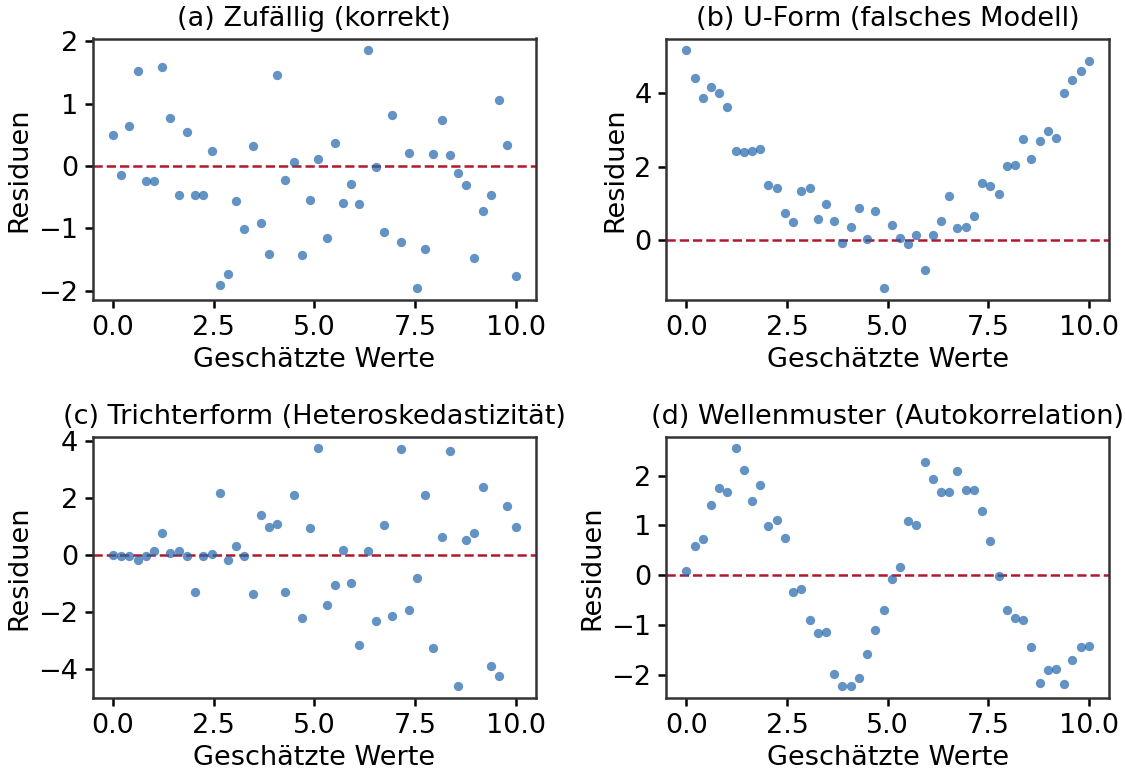
\includegraphics[width=0.9\textwidth,height=0.8\textheight,keepaspectratio]{images/image_022.png}
  \end{center}
\end{frame}

% Slide 137: Residuenplot Beispiel - Image only
\begin{frame}{Residuenplot -- Beispiel}
  \begin{center}
    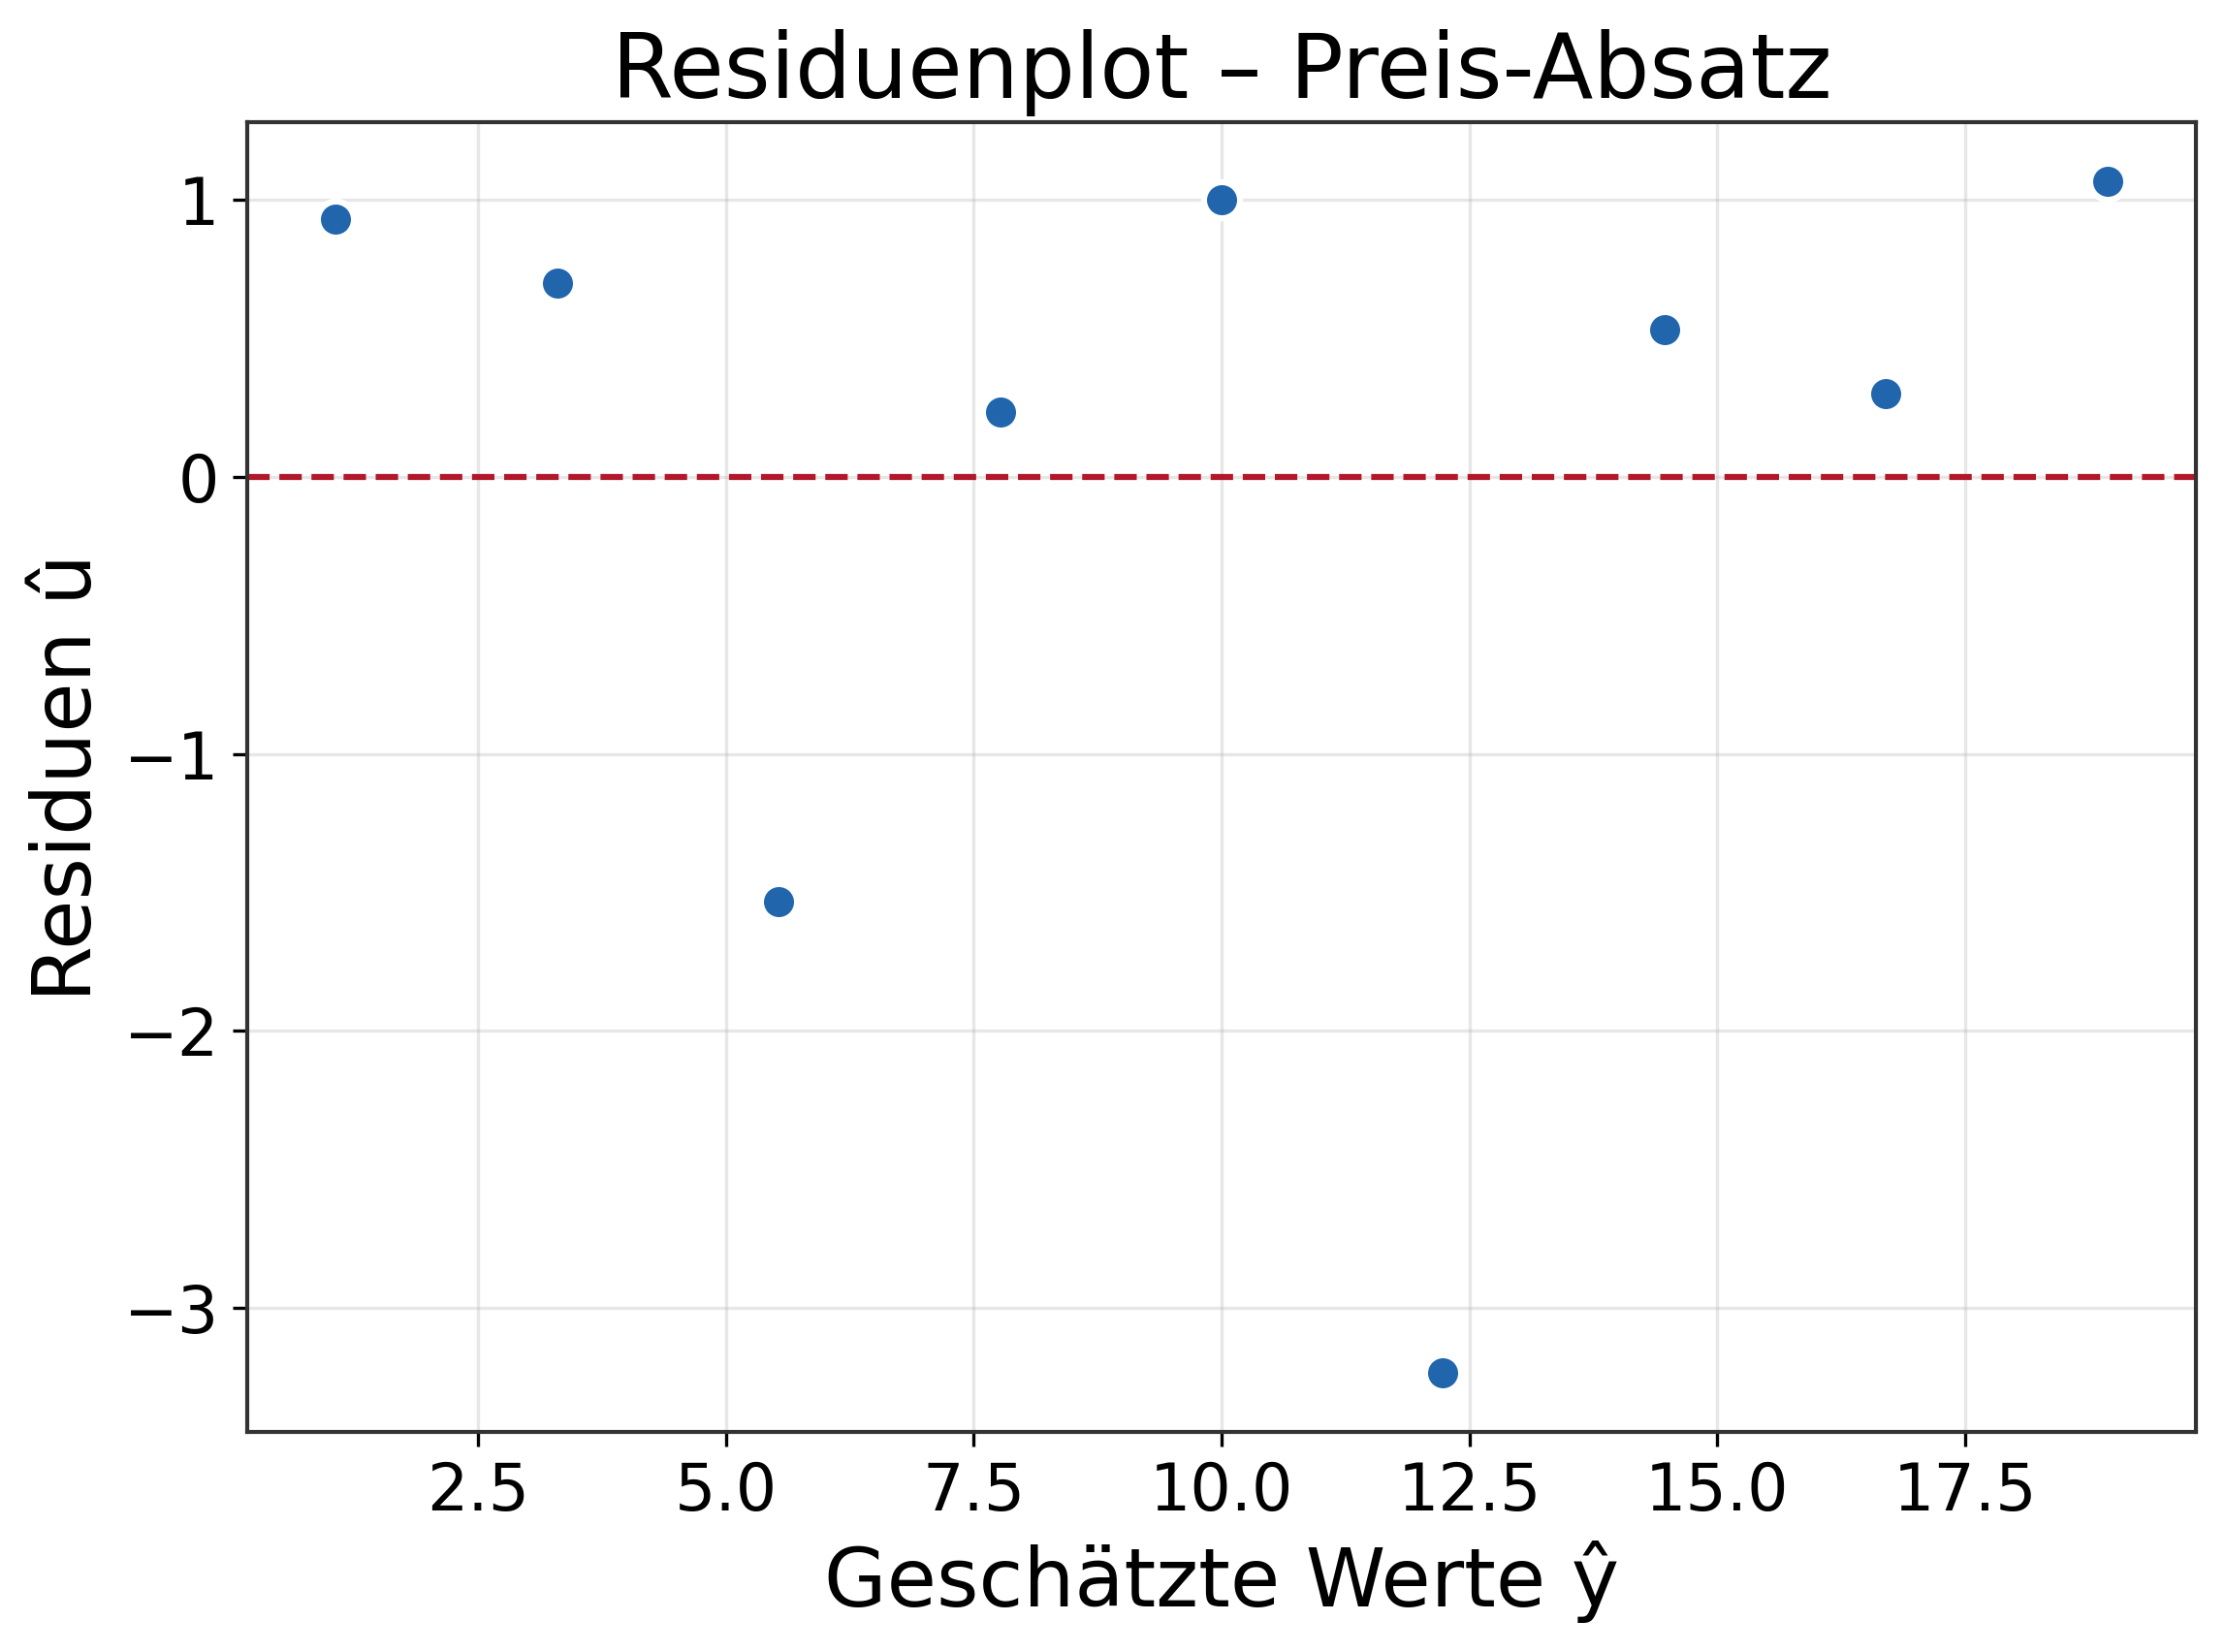
\includegraphics[width=0.8\textwidth,height=0.75\textheight,keepaspectratio]{images/image_023.png}
  \end{center}
\end{frame}

% Slide 138: Residuenplot Beispiel - mit Interpretation
\begin{frame}{Residuenplot -- Beispiel (Interpretation)}
  \begin{center}
    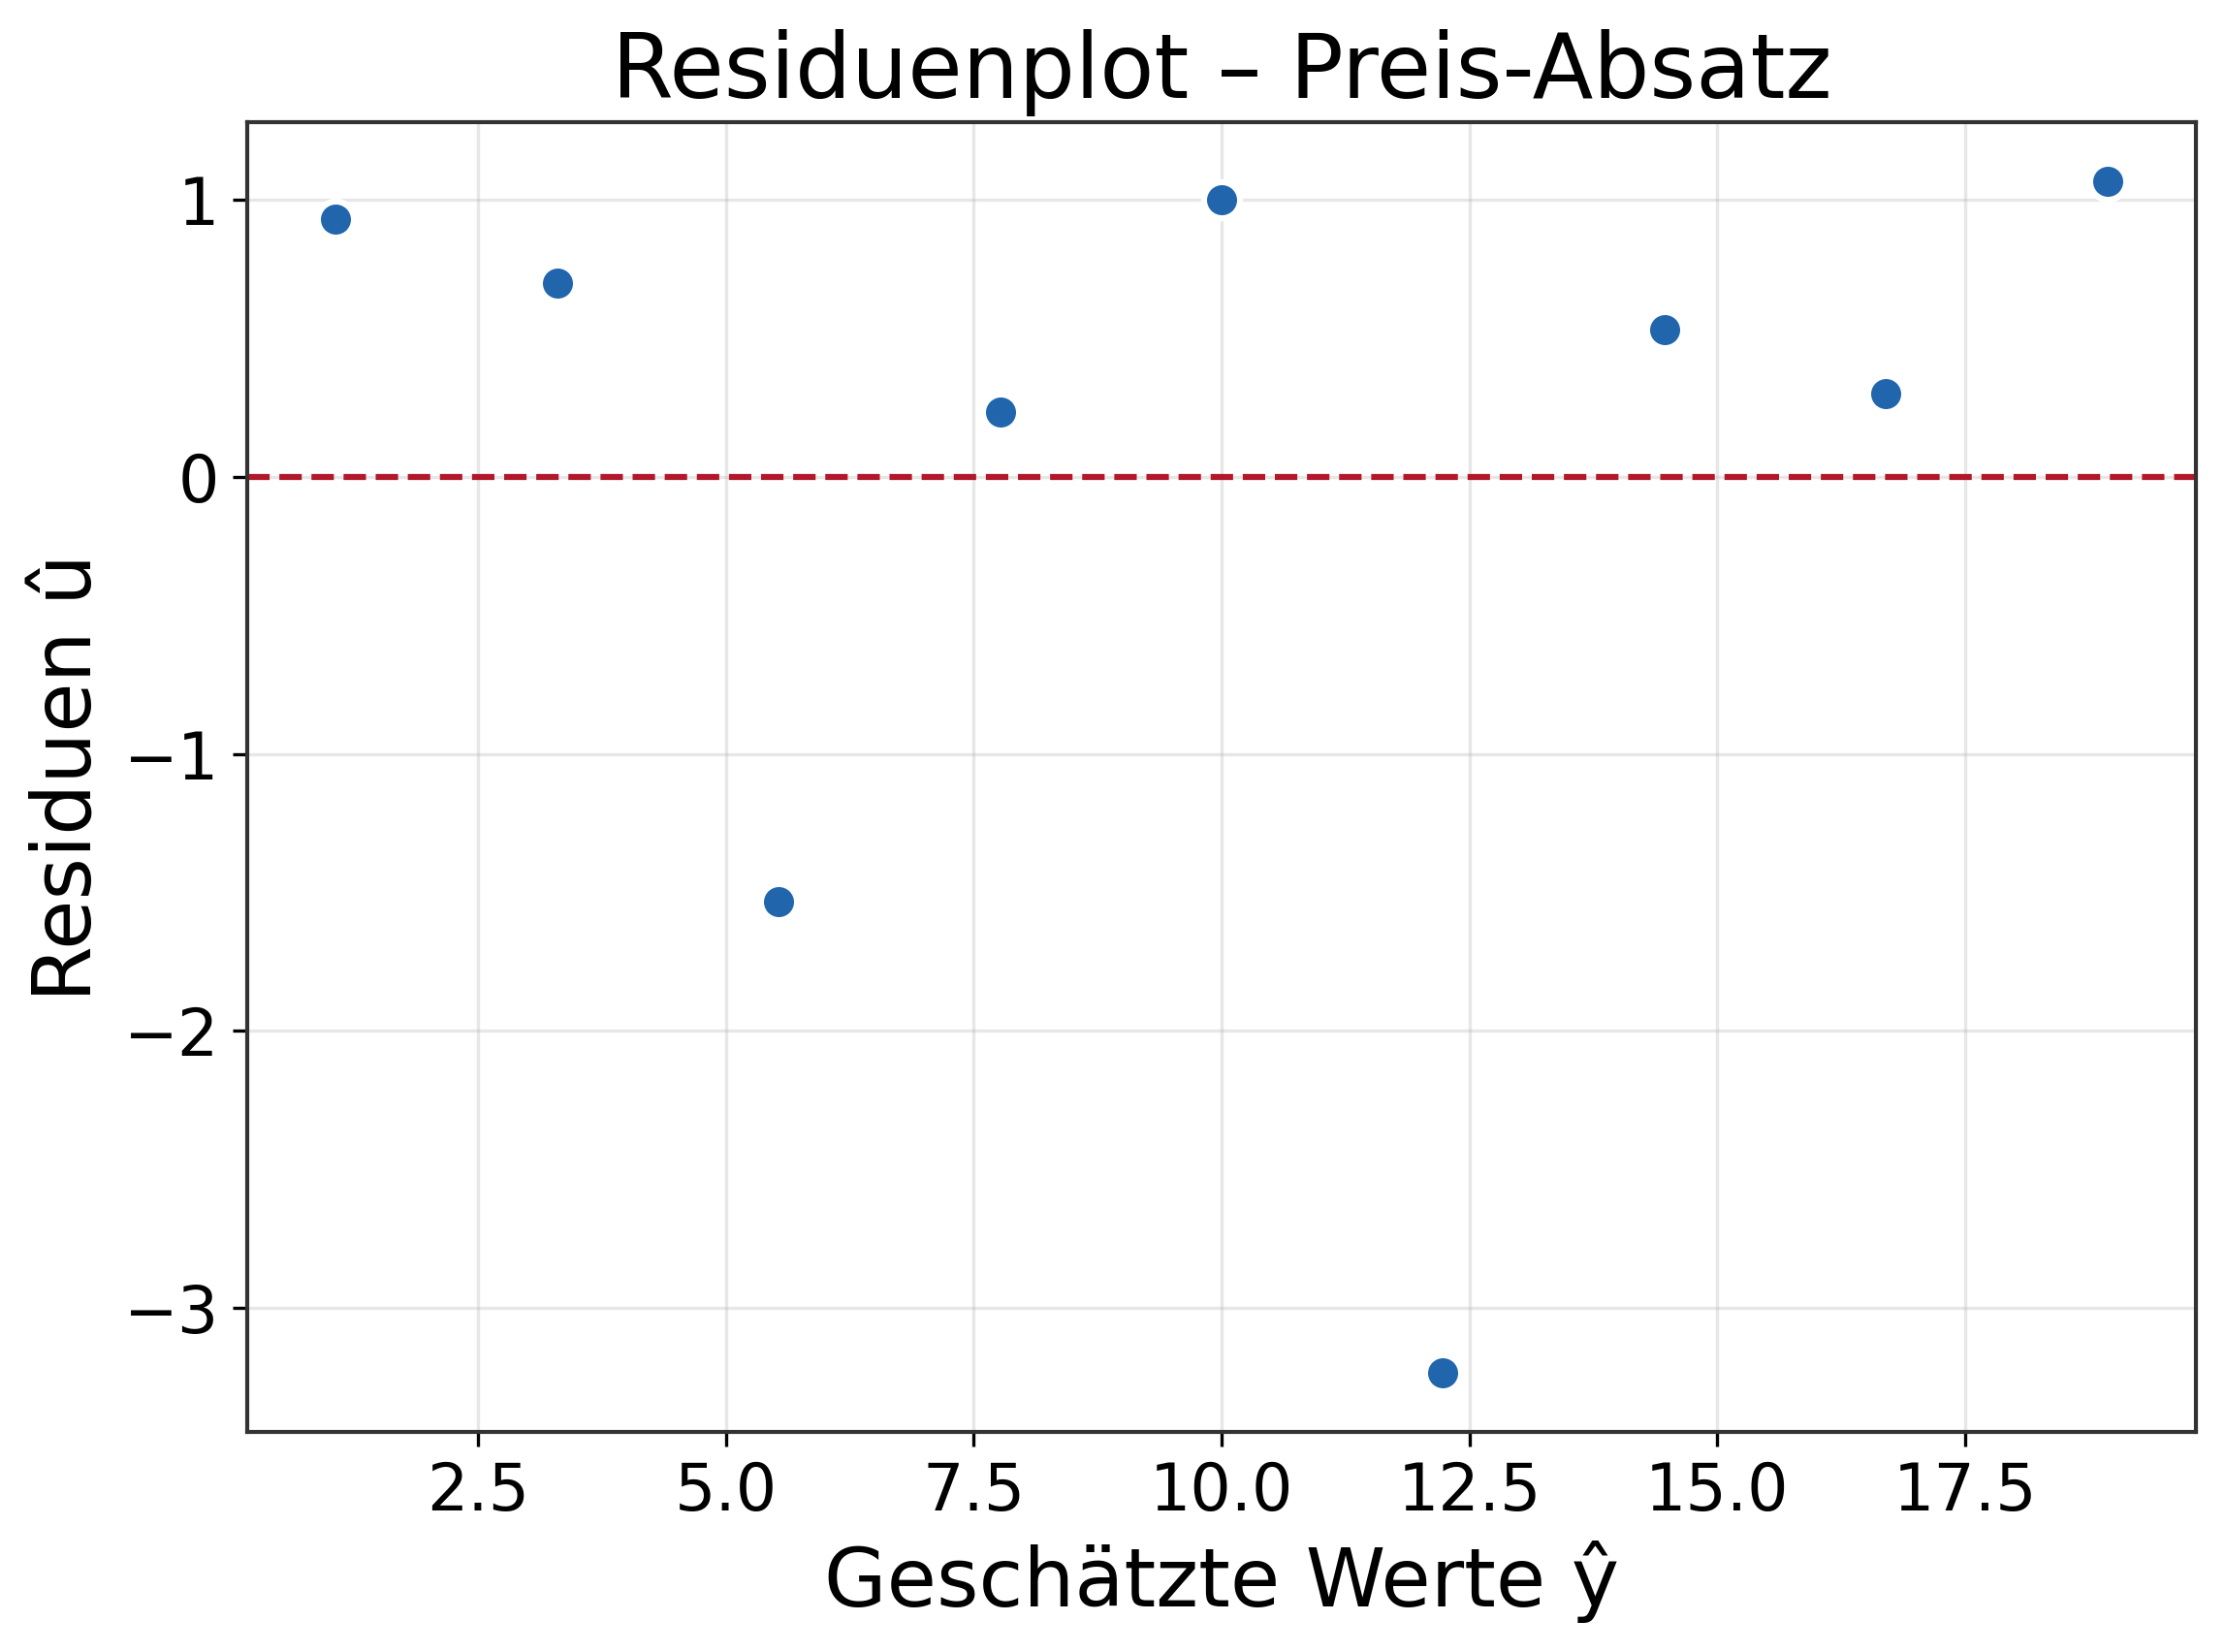
\includegraphics[width=0.8\textwidth,height=0.75\textheight,keepaspectratio]{images/image_023.png}
  \end{center}

  Keine Systematik erkennbar.
\end{frame}

% Slide 139: Residuenplot mit R
\begin{frame}[fragile]{Residuenplot mit R erstellen}
  \footnotesize
  \lstset{basicstyle=\ttfamily\footnotesize}
  \begin{block}{R-Befehle}
\begin{lstlisting}
reg <- lm(menge ~ preis)
plot(fitted(reg), resid(reg))
abline(h = 0, lty = 2)                  # Nulllinie als Orientierung
\end{lstlisting}
  \end{block}

  \begin{block}{Hilfsfunktionen}
    \begin{description}\setlength{\itemsep}{0pt}\setlength{\parsep}{0pt}\setlength{\topsep}{0pt}
      \item[\texttt{fitted(reg)}] gibt die geschätzten Werte
            $\hat{y}_i = \hat{\beta}_0 + \hat{\beta}_1 x_i$ aus
            -- Werte auf der $x$-Achse.
      \item[\texttt{resid(reg)}] gibt die Residuen
            $\hat{u}_i = y_i - \hat{y}_i$ aus
            -- Werte auf der $y$-Achse.
    \end{description}
  \end{block}

  \begin{exampleblock}{Lesbarer gestalten}
\begin{lstlisting}
plot(fitted(reg), resid(reg),
     xlab = "geschaetzte Werte", ylab = "Residuen", main = "Residuenplot")
abline(h = 0, lty = 2)
\end{lstlisting}
  \end{exampleblock}
\end{frame}

% ===== SUBSECTION: QQ-PLOT =====
\subsection{QQ-Plot}

% ---- Slide 140: QQ-Plot Subsection-Intro -------------------
\begin{frame}{QQ-Plot}
  \begin{block}{Annahme}
    Die Residuen der linearen Regression sind \textbf{normalverteilt}.
  \end{block}

  \begin{exampleblock}{Werkzeug zur Überprüfung}
    Überprüfung der Normalverteilung mit Hilfe eines \textbf{QQ-Plots}
    (Quantil-Quantil-Diagramm).
  \end{exampleblock}
\end{frame}

% ---- Slide 141: Was ist ein QQ-Plot? -----------------------
\begin{frame}{Was ist ein QQ-Plot?}
  \begin{block}{Definition}
    Der \emph{QQ-Plot} ist eine \textbf{Quantils-Quantils-Grafik}: Die
    Quantile (oft in $5\,\%$- oder $1\,\%$-Schritten) der beiden
    Merkmale werden auf den beiden Achsen gegeneinander abgetragen.
  \end{block}

  \begin{block}{Aufbau und Referenzlinie}
    Anhand des QQ-Plots kann festgestellt werden, wie ähnlich die
    beiden Verteilungen sind. Zum besseren Vergleich wird eine
    \textbf{Verbindungslinie zwischen dem $25\,\%$- und dem $75\,\%$-Quantil}
    eingezeichnet.
  \end{block}

  \begin{alertblock}{Interpretation}
    Je weiter die einzelnen Punkte von der Geraden entfernt liegen,
    \textbf{desto unähnlicher} sind die beiden Verteilungen. Liegen
    alle Punkte auf der Geraden, sind die Verteilungen identisch.
  \end{alertblock}
\end{frame}

% ---- Slide 142: Beispiel - Daten ---------------------------
\begin{frame}{Was ist ein QQ-Plot? -- Beispiel}
  \begin{block}{Leuchte-Preis-Absatz-Beispiel}
    Wir betrachten erneut unser Leuchte-Preis-Absatz-Beispiel aus der
    Regression mit Preis $x$ und Absatz $y$:
    \begin{center}
      \begin{tabular}{lrrrrrrrrr}
        \toprule
        $x$ (Preis)  & 80 & 85 & 90 & 95 & 100 & 105 & 110 & 115 & 120 \\
        $y$ (Absatz) & 20 & 17 & 15 & 9  & 11  & 8   & 4   & 4   & 2   \\
        \bottomrule
      \end{tabular}
    \end{center}
  \end{block}

  \begin{block}{Schritt 1 -- Daten sortieren}
    Zunächst werden die Daten von $x$ und $y$ \textbf{getrennt
    aufsteigend sortiert}:
    \begin{center}
      \begin{tabular}{lrrrrrrrrr}
        \toprule
        $x^{\text{sort}}$ & 80 & 85 & 90 & 95 & 100 & 105 & 110 & 115 & 120 \\
        $y^{\text{sort}}$ & 2  & 4  & 4  & 8  & 9   & 11  & 15  & 17  & 20  \\
        \bottomrule
      \end{tabular}
    \end{center}
    Daraus wird eine Grafik erstellt, in der die Punktepaare
    $(x_i^{\text{sort}}, y_i^{\text{sort}})$ eingetragen werden.
  \end{block}
\end{frame}

% ---- Slide 143/144: QQ-Plot Preis-Absatz Grafik ------------
\begin{frame}{Was ist ein QQ-Plot? -- Beispiel (Grafik)}
  \begin{center}
    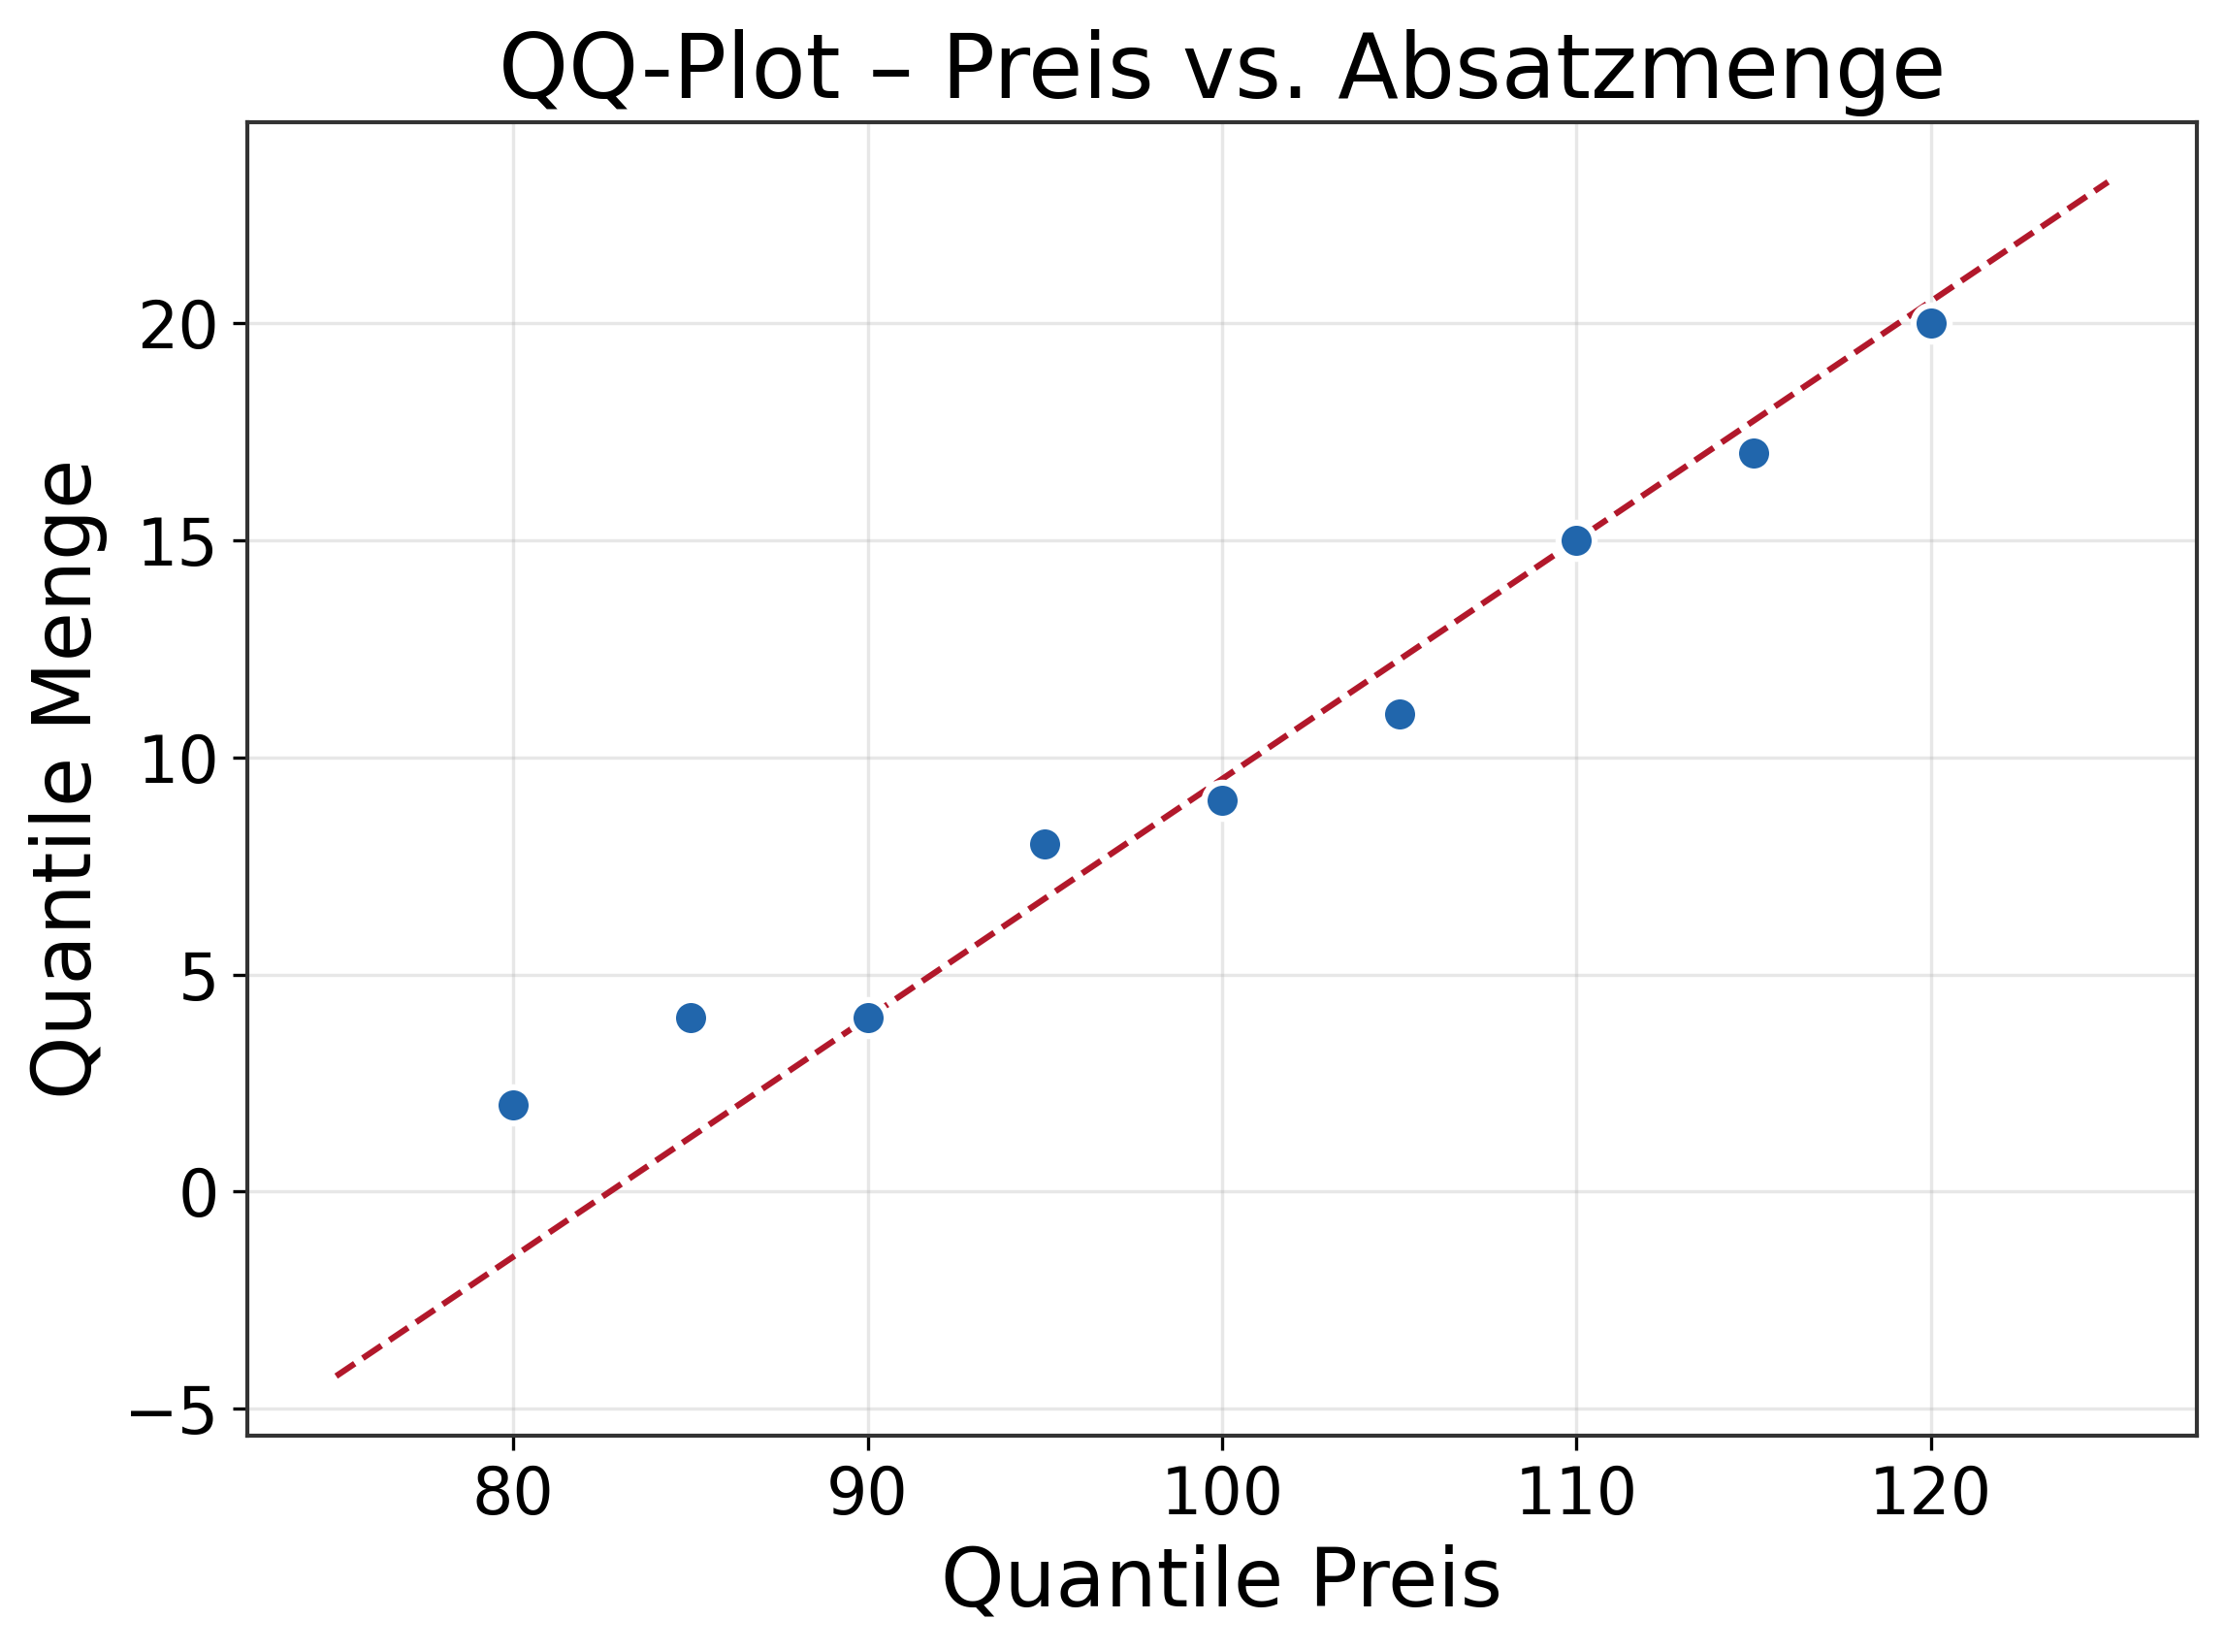
\includegraphics[width=0.85\textwidth,height=0.78\textheight,keepaspectratio]{images/image_024.png}
  \end{center}
\end{frame}

% ---- Slide 145: QQ-Plot mit R erzeugen ---------------------
\begin{frame}[fragile]{QQ-Plot mit R erzeugen}
  \begin{block}{QQ-Plot zeichnen}
\begin{lstlisting}
qqplot(preis, menge)
\end{lstlisting}
  \end{block}

  \begin{block}{Gerade in den QQ-Plot zeichnen}
\begin{lstlisting}
qqline(menge,
       distribution = function(p) quantile(preis, prob = p),
       lty = 2)
\end{lstlisting}
  \end{block}

  \begin{exampleblock}{Idee}
    Die Funktion \texttt{qqplot()} erzeugt das QQ-Diagramm für die
    \emph{empirischen} Verteilungen der beiden Stichproben;
    \texttt{qqline()} ergänzt eine Referenzgerade durch das $25\,\%$-
    und das $75\,\%$-Quantil.
  \end{exampleblock}
\end{frame}

% ---- Slide 146: Überprüfung der Normalverteilung ----------
\begin{frame}{Überprüfung der Normalverteilung der Residuen mithilfe des QQ-Plots}
  \begin{block}{Ausgangslage}
    \textbf{Annahme:} Die Residuen der linearen Regression sind
    normalverteilt, $u_i \sim \mathcal{N}(0,\sigma^{2})$.
  \end{block}

  \begin{exampleblock}{Idee}
    Wir verwenden den QQ-Plot, um die empirische Verteilung der
    Residuen mit der theoretischen \textbf{Standard\-normal\-verteilung}
    zu vergleichen.
  \end{exampleblock}
\end{frame}

% ---- Slide 147: Untersuchung der Residuen mit dem QQ-Plot --
\begin{frame}{Untersuchung der Residuen mit dem QQ-Plot}
  \begin{block}{QQ-Plot Stichprobe vs.\ Theorie}
    Der QQ-Plot kann auch zwischen einer Stichprobenverteilung und
    einer \emph{theoretischen} Verteilung wie der Normalverteilung
    gezeichnet werden. Damit wird die Ähnlichkeit zwischen
    Stichprobe und Normalverteilung festgestellt.
  \end{block}

  \begin{block}{Konstruktion}
    \begin{description}
      \item[$y$-Achse] sortierte Werte der Residuen $\hat{u}_{(i)}$
      \item[$x$-Achse] Quantile $z_i$ der Standardnormalverteilung
    \end{description}
    Die theoretischen Quantile werden über
    \begin{center}
      $\displaystyle
        \Pr(x < z_i) \;=\; \frac{i - 0{,}5}{n},
        \qquad z_i = \Phi^{-1}\!\left(\tfrac{i-0{,}5}{n}\right)
      $
    \end{center}
    ermittelt.
  \end{block}
\end{frame}

% ---- Slide 148: Untersuchung Residuen - Beispiel Tabelle ---
\begin{frame}{Untersuchung der Residuen mit dem QQ-Plot -- Beispiel}
  \begin{center}
    \small
    \begin{tabular}{rrrrr}
      \toprule
      \textbf{Residuum $\hat{u}_i$} & \textbf{$\hat{u}_{(i)}$ sortiert} & \textbf{Index $i$} & \textbf{$\Pr(z<Z) = \tfrac{i-0{,}5}{n}$} & \textbf{Quantil $z_i$} \\
      \midrule
       $1{,}06666667$ & $-3{,}23333333$ & 1 & $0{,}05555556$ & $-1{,}59321882$ \\
       $0{,}30000000$ & $-1{,}53333333$ & 2 & $0{,}16666667$ & $-0{,}96742157$ \\
       $0{,}53333333$ &  $0{,}23333333$ & 3 & $0{,}27777778$ & $-0{,}58945580$ \\
      $-3{,}23333333$ &  $0{,}30000000$ & 4 & $0{,}38888889$ & $-0{,}28221615$ \\
       $1{,}00000000$ &  $0{,}53333333$ & 5 & $0{,}50000000$ &  $0{,}00000000$ \\
       $0{,}23333333$ &  $0{,}70000000$ & 6 & $0{,}61111111$ &  $0{,}28221615$ \\
      $-1{,}53333333$ &  $0{,}93333333$ & 7 & $0{,}72222222$ &  $0{,}58945580$ \\
       $0{,}70000000$ &  $1{,}00000000$ & 8 & $0{,}83333333$ &  $0{,}96742157$ \\
       $0{,}93333333$ &  $1{,}06666667$ & 9 & $0{,}94444444$ &  $1{,}59321882$ \\
      \bottomrule
    \end{tabular}
  \end{center}
\end{frame}

% ---- Slide 149: Untersuchung Residuen - Grafik -------------
\begin{frame}{Untersuchung der Residuen mit dem QQ-Plot -- Beispiel}
  \begin{center}
    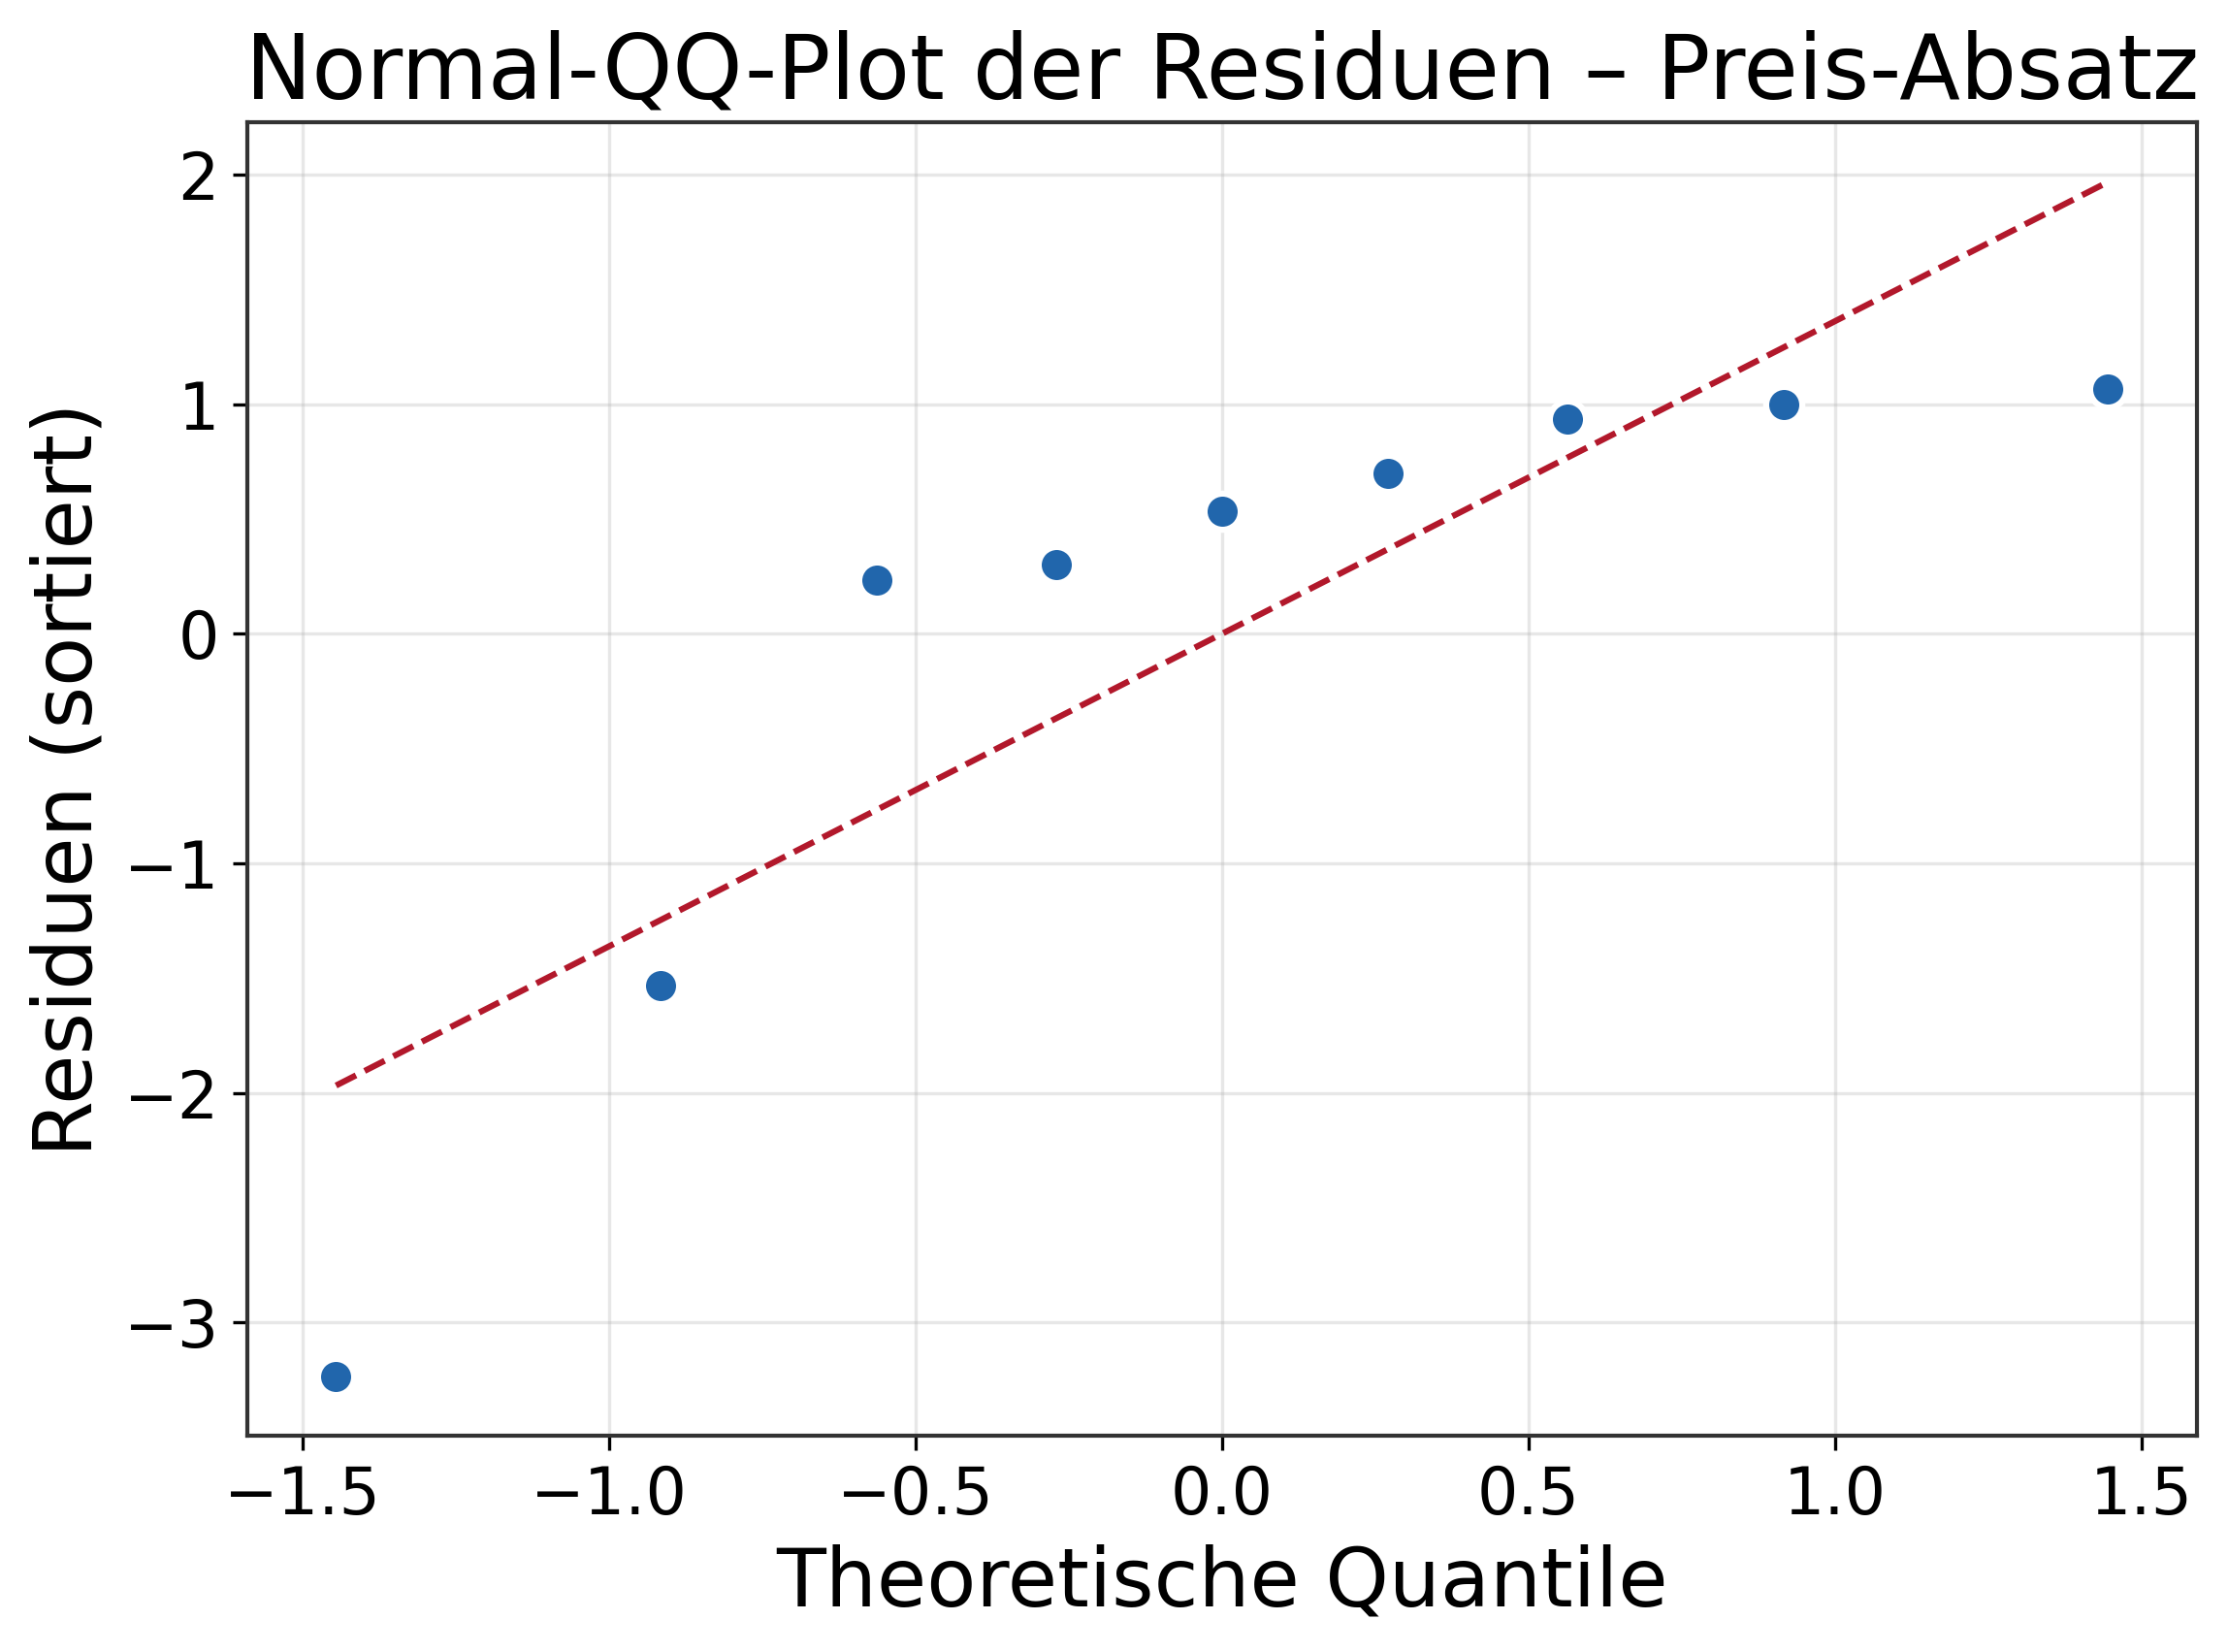
\includegraphics[width=0.8\textwidth,height=0.78\textheight,keepaspectratio]{images/image_025.png}
  \end{center}
\end{frame}

% ---- Slide 150: Beispiel + Interpretation ------------------
\begin{frame}{Untersuchung der Residuen mit dem QQ-Plot -- Interpretation}
  \begin{columns}[T]
    \begin{column}{0.50\textwidth}
      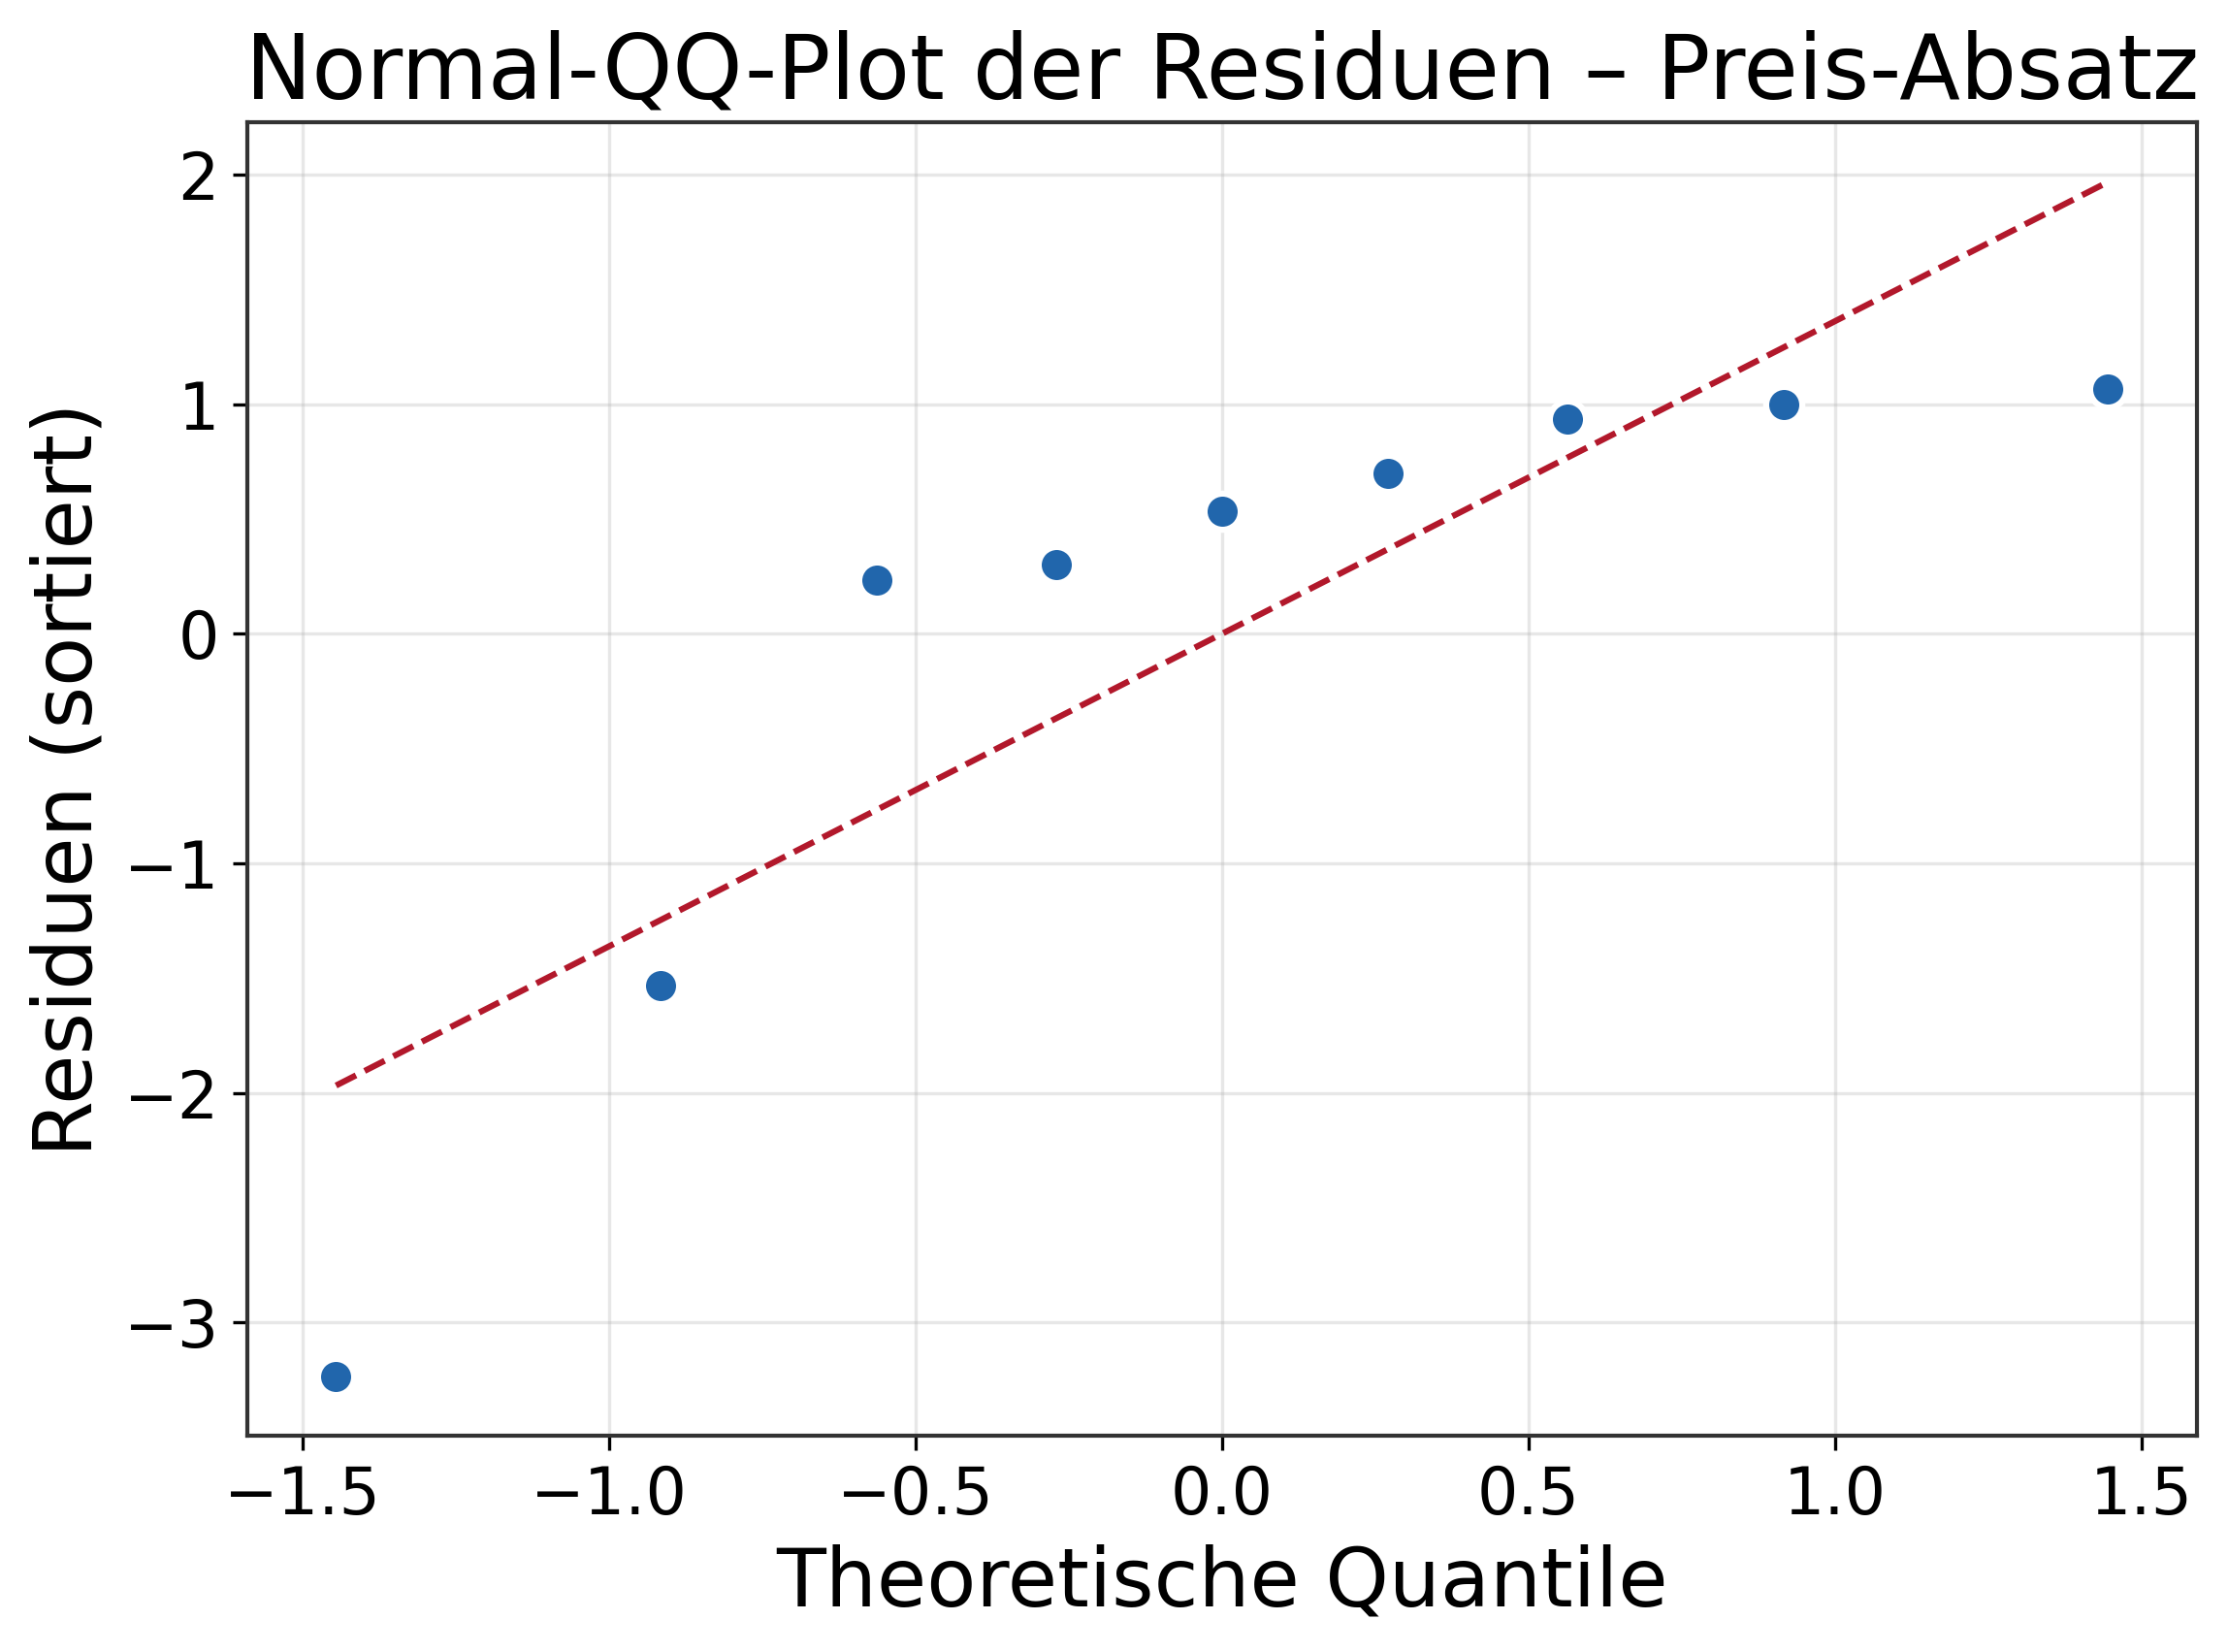
\includegraphics[width=\textwidth,height=0.78\textheight,keepaspectratio]{images/image_025.png}
    \end{column}
    \begin{column}{0.46\textwidth}
      \begin{block}{Beobachtung}
        \textbf{In der Mitte} gute Anlehnung an die Normalverteilung.
        \textbf{Am unteren Rand} nicht normalverteilt.
      \end{block}

      \begin{alertblock}{Vorsicht}
        $n=9$ -- das sind nur sehr wenige Daten!
      \end{alertblock}
    \end{column}
  \end{columns}
\end{frame}

% ---- Slide 151: Beispiel + Conclusion ----------------------
\begin{frame}{Untersuchung der Residuen mit dem QQ-Plot -- Fazit}
  \begin{columns}[T]
    \begin{column}{0.50\textwidth}
      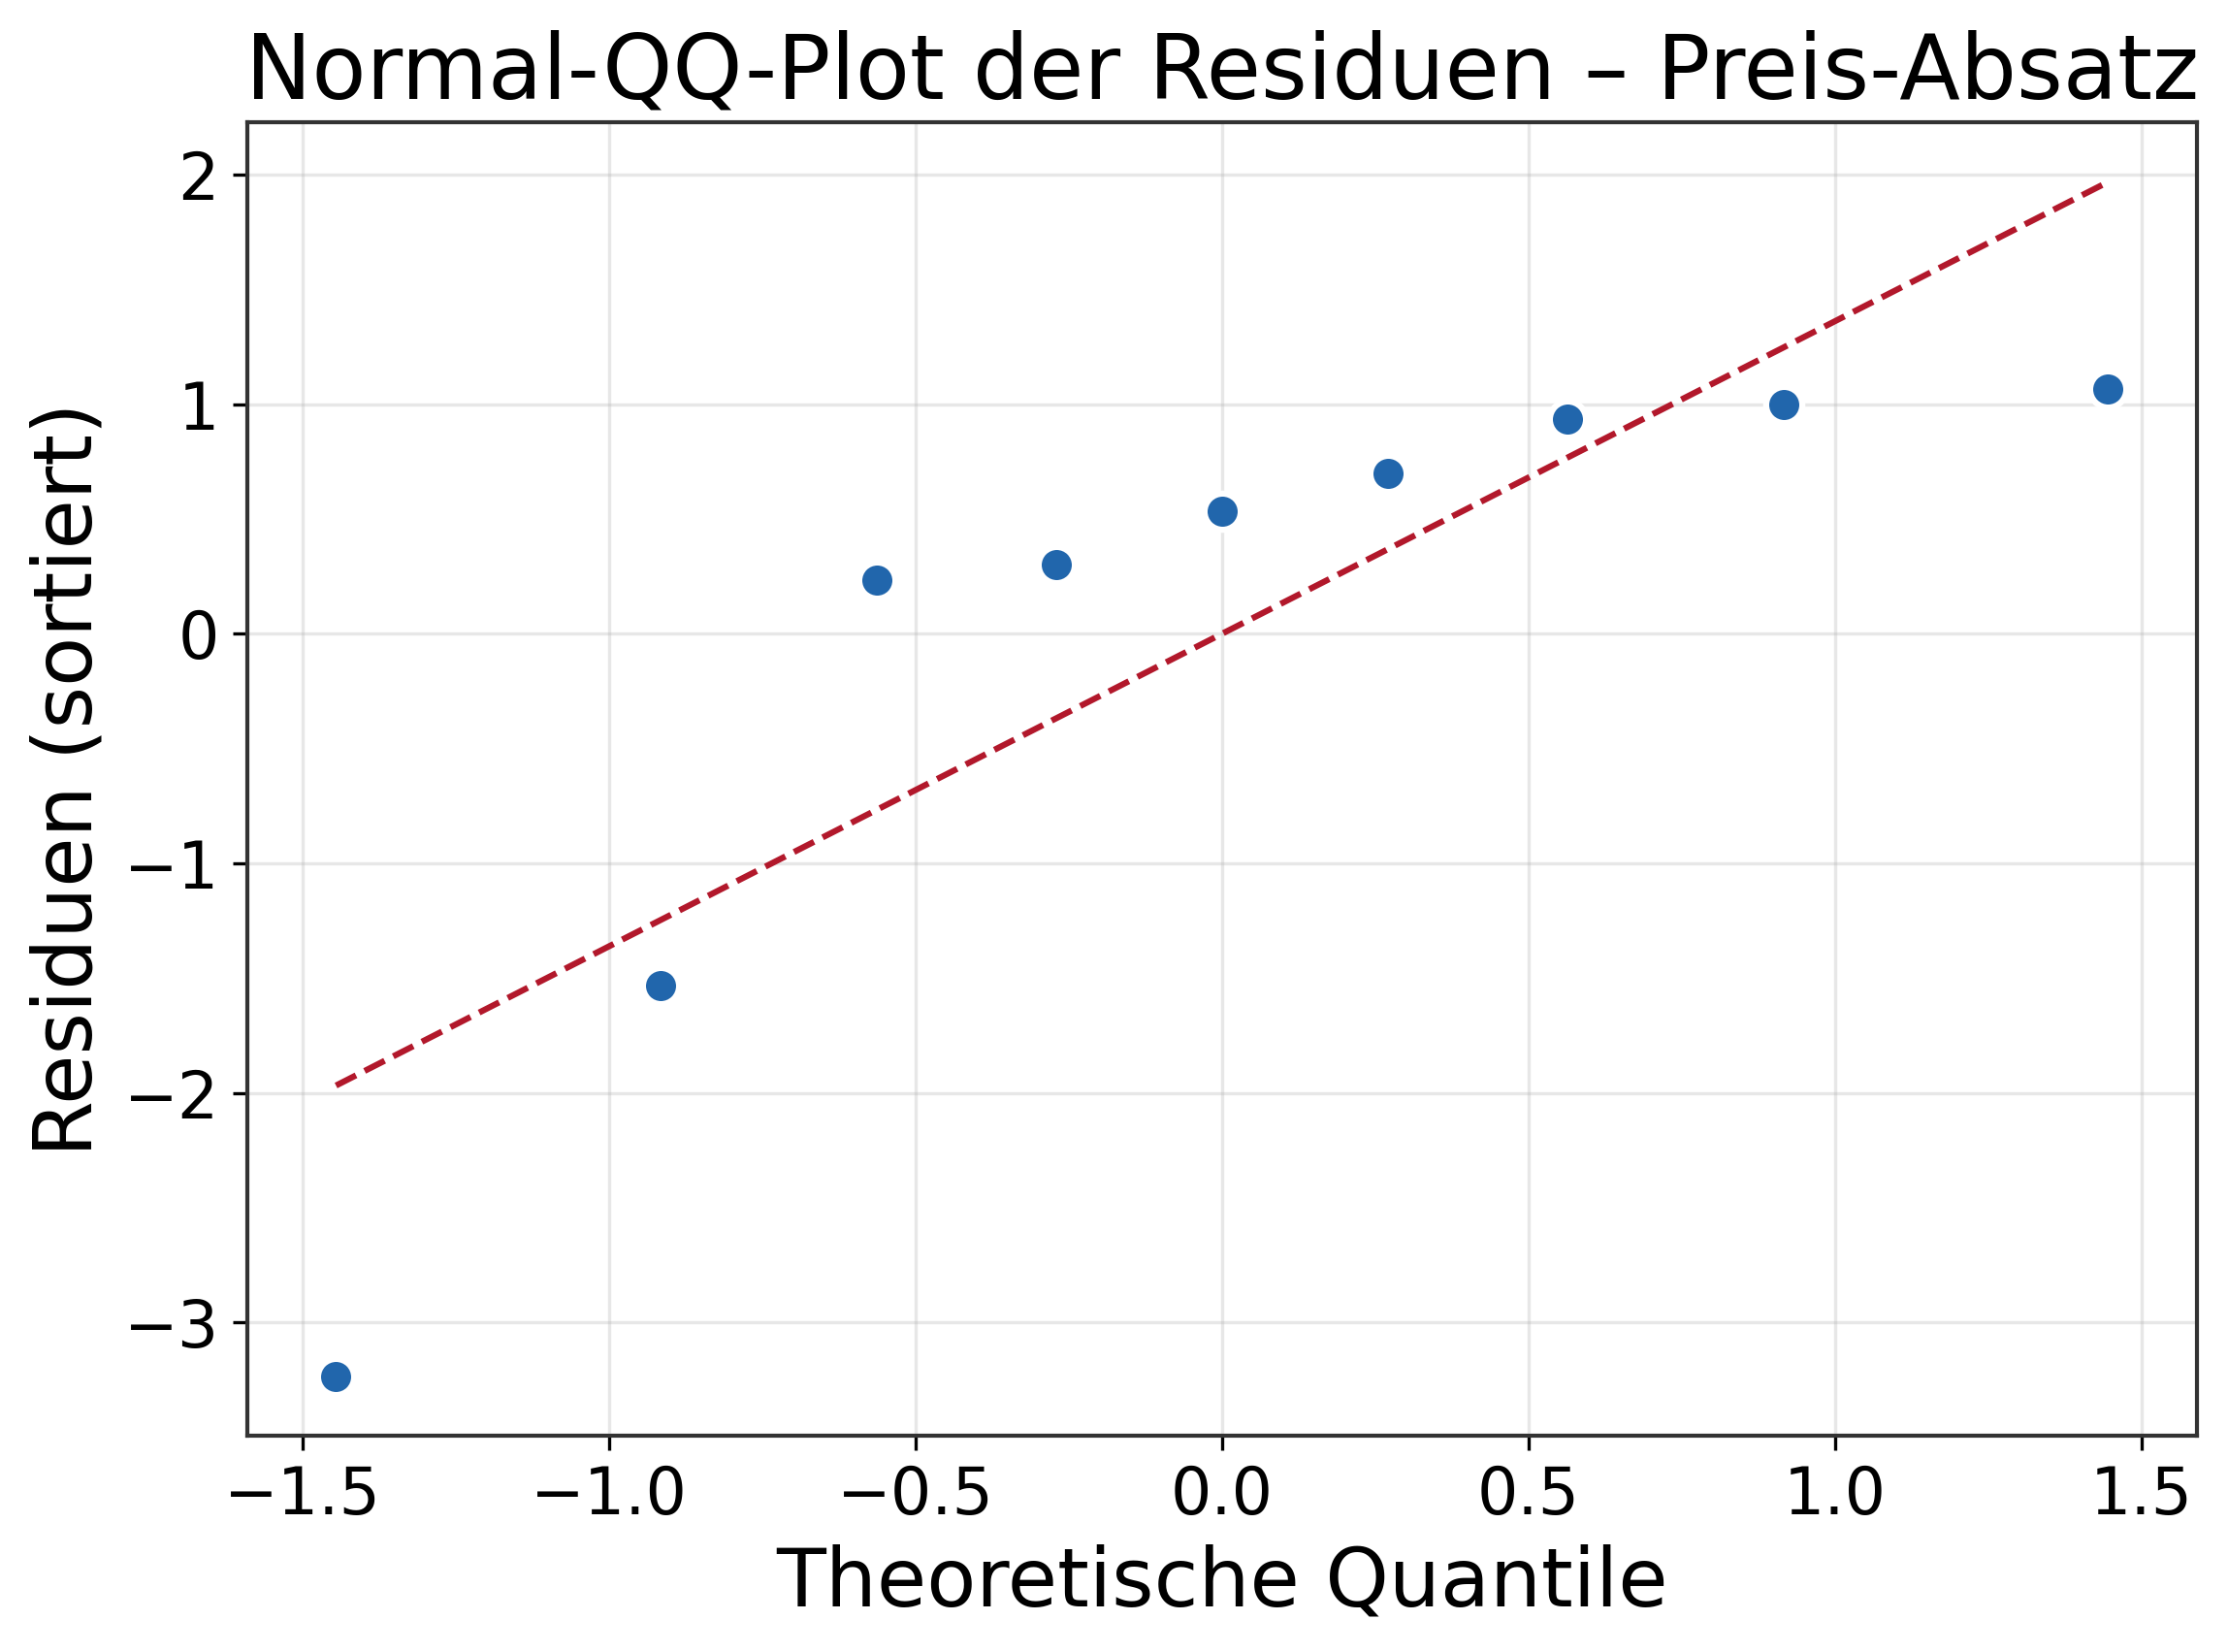
\includegraphics[width=\textwidth,height=0.78\textheight,keepaspectratio]{images/image_025.png}
    \end{column}
    \begin{column}{0.46\textwidth}
      \begin{block}{Beobachtung}
        \textbf{In der Mitte} gute Anlehnung an die Normalverteilung.
        \textbf{Am unteren Rand} nicht normalverteilt.
      \end{block}

      \begin{alertblock}{Fazit}
        $n=9$ -- nur sehr wenige Daten! Vorsicht!\\[0.3em]
        \textbf{Nicht normalverteilt!}
      \end{alertblock}
    \end{column}
  \end{columns}
\end{frame}

% ---- Slide 152: QQ-Plot Residuen gegen Normalverteilung in R
\begin{frame}[fragile]{QQ-Plot der Residuen gegen Normalverteilung in R erzeugen}
  \begin{block}{QQ-Plot erzeugen}
\begin{lstlisting}
qqnorm(resid(reg))
\end{lstlisting}
  \end{block}

  \begin{block}{Gerade zwischen den Quartilen einzeichnen}
\begin{lstlisting}
qqline(resid(reg))
\end{lstlisting}
  \end{block}

  \begin{exampleblock}{Was die Befehle tun}
    \texttt{qqnorm()} berechnet intern die Plotting-Positionen
    $p_i = (i-0{,}5)/n$, die Normalquantile
    $z_i = \Phi^{-1}(p_i)$ und zeichnet die Paare
    $(z_i, \hat{u}_{(i)})$. \texttt{qqline()} legt eine
    Referenzgerade durch das $25\,\%$- und $75\,\%$-Quantil.
  \end{exampleblock}
\end{frame}

% ===== SUBSECTION: BESTIMMTHEITSMAS =====
\subsection{Bestimmtheitsmaß}

% ---- Slide 153: Streuungszerlegung -- Idee -----------------
\begin{frame}{Streuungszerlegung}
  \begin{block}{Idee}
    Die Regression zerlegt die Varianz $s_y^{\,2}$ in eine Varianz
    \emph{auf} der Regressionsgeraden $s_{\hat{y}}^{\,2}$ und eine
    Varianz \emph{um} die Regressionsgerade $s_{\hat{u}}^{\,2}$,
    welche auch als die \textbf{Residuenvarianz} bezeichnet wird.
  \end{block}

  \begin{exampleblock}{Streuungszerlegung}
    \begin{center}
      $\displaystyle s_y^{\,2} \;=\; s_{\hat{y}}^{\,2} \;+\; s_{\hat{u}}^{\,2}$
    \end{center}
    Diese Zerlegung der Varianz wird als \textbf{Streuungszerlegung}
    oder \textbf{Varianzanalyse} bezeichnet.
  \end{exampleblock}

  \begin{block}{In Worten}
    (Gesamtvarianz von $y$) $=$ (erklärte Varianz von $y$) $+$
    Residuenvarianz
  \end{block}
\end{frame}

% ---- Slide 153b: Streuungszerlegung -- Quadratsummenform ---
\begin{frame}{Streuungszerlegung -- Quadratsummen und Varianzen}
  \begin{block}{Quadratsummenzerlegung}
    \begin{center}
      $\displaystyle
        \underbrace{\sum_{i=1}^{n} (y_i - \bar{y})^2}_{\text{SQT (total)}}
        \;=\;
        \underbrace{\sum_{i=1}^{n} (\hat{y}_i - \bar{y})^2}_{\text{SQE (erklärt)}}
        \;+\;
        \underbrace{\sum_{i=1}^{n} \hat{u}_i^{\,2}}_{\text{SQR (Residuen)}}$
    \end{center}
  \end{block}

  \begin{exampleblock}{In Varianzen}
    Teilen durch $n$ liefert die Zerlegung der Varianzen:
    \begin{center}
      $\displaystyle s_y^{\,2} \;=\; s_{\hat{y}}^{\,2} \;+\; s_{\hat{u}}^{\,2}$
    \end{center}
    \begin{description}
      \item[$s_y^{\,2}$] Gesamtvarianz von $y$
      \item[$s_{\hat{y}}^{\,2}$] durch die Regression \emph{erklärte} Varianz
      \item[$s_{\hat{u}}^{\,2}$] \emph{Residuenvarianz} (unerklärter Teil)
    \end{description}
  \end{exampleblock}
\end{frame}

% ---- Slide 154: Streuungszerlegung -- Zusammenhang KQ ------
\begin{frame}{Streuungszerlegung -- Zusammenhang zur Kleinst-Quadrate-Methode}
  \begin{block}{Ausgangspunkt}
    Die Varianz \emph{um} die Regressionsgerade ist der nicht durch
    die Regression zu erklärende Anteil an der Gesamtvarianz. Es ist
    die Varianz der Residuen $s_{\hat{u}}^{\,2}$. Die Regressions\-koeffizienten
    werden mit dem Ansatz der \textbf{Minimierung der Residuenvarianz}
    berechnet (Kleinst-Quadrate-Ansatz). Daher ist diese Varianz
    \textbf{minimal}.
  \end{block}

  \begin{exampleblock}{Folge für die Streuungszerlegung}
    \begin{center}
      $\displaystyle
        \underbrace{s_y^{\,2}}_{\text{fest}}
        \;=\;
        \underbrace{s_{\hat{y}}^{\,2}}_{\text{\color{green!55!black}maximal}}
        \;+\;
        \underbrace{s_{\hat{u}}^{\,2}}_{\text{\color{red!70!black}minimal}}$
    \end{center}
    $\Rightarrow$ Die durch die Regressionsgerade \textbf{erklärte
    Varianz} $s_{\hat{y}}^{\,2}$ ist \textbf{maximal}.\\[0.4em]
    (Gesamtvarianz von $y$) $=$ (erklärte Varianz von $y$) $+$
    Residuenvarianz
  \end{exampleblock}
\end{frame}

% ---- Slide 155: Bestimmtheitsmaß -- Definition -------------
\begin{frame}{Bestimmtheitsmaß}
  \begin{block}{Definition}
    Das \textbf{Bestimmtheitsmaß} $R^{2}$ ist das Verhältnis der
    Varianz auf der Regressionsgeraden zur Gesamtvarianz:
    \begin{center}
      $\displaystyle
        R^{2} \;=\; \frac{s_{\hat{y}}^{\,2}}{s_y^{\,2}}
        \qquad 0 \le R^{2} \le 1.$
    \end{center}
  \end{block}

  \begin{exampleblock}{Interpretation}
    Das Bestimmtheitsmaß gibt den \emph{Anteil} der Gesamtvarianz an,
    der durch die Regressionsbeziehung erklärt wird.
  \end{exampleblock}
\end{frame}

% ---- Slide 155b: Bestimmtheitsmaß -- Extremfälle -----------
\begin{frame}{Bestimmtheitsmaß -- Extremfälle}
  \begin{block}{$R^{2} = 1$: perfekte Anpassung}
    Mit der Regression wird die \emph{gesamte} Varianz von $y$
    erklärt. Es existieren keine Werte ober- und unterhalb der
    Regressionsgeraden. \textbf{Die Werte liegen alle auf der
    Regressionsgerade.} Es gibt keine Residuen: $s_{\hat{u}}^{\,2} = 0$.
  \end{block}

  \begin{alertblock}{$R^{2} = 0$: keine erklärte Varianz}
    Mit der Regressionsgeraden wird keine Varianz erklärt:
    $s_{\hat{y}}^{\,2} = 0$. \textbf{Die Regressionsgerade besitzt
    keine Steigung} ($\hat{\beta}_1 = 0$) und verläuft in Höhe des
    Mittelwerts $\bar{y}$.
  \end{alertblock}

  \begin{exampleblock}{Faustregel}
    Je näher $R^{2}$ bei $1$ liegt, desto besser erklärt das lineare
    Modell die Daten. Ein niedriges $R^{2}$ bedeutet nicht, dass $X$
    und $Y$ unabhängig sind -- sondern nur, dass der \emph{lineare}
    Zusammenhang schwach ist.
  \end{exampleblock}
\end{frame}

% ---- Slide 155c: Erklärte Varianz -- Ausgangspunkt -----------
\begin{frame}{Erklärte Varianz -- Ausgangspunkt}
  \begin{block}{Lineare Form der Schätzwerte}
    Die geschätzten Werte sind linear in $x_i$:
    \[
      \hat{y}_i \;=\; \hat{\beta}_0 \,+\, \hat{\beta}_1\, x_i.
    \]
  \end{block}

  \begin{exampleblock}{Ziel der nächsten Folien}
    Wir zeigen die nützliche Identität
    \[
      s_{\hat{y}}^{\,2} \;=\; \hat{\beta}_1^{\,2}\, s_x^{\,2},
    \]
    aus der unmittelbar die alternative Formel für $R^{2}$ folgt.
  \end{exampleblock}
\end{frame}

% ---- Slide 155d: Herleitung -- Mittelwert und Differenz ------
\begin{frame}{Herleitung -- Mittelwert und Differenz}
  \begin{block}{Schritt 1: Mittelwert von $\hat{y}$}
    Da $\hat{\beta}_0$ und $\hat{\beta}_1$ Konstanten sind, gilt:
    \[
      \bar{\hat{y}}
        \;=\; \tfrac{1}{n}\sum_{i=1}^{n}\hat{y}_i
        \;=\; \hat{\beta}_0 \,+\, \hat{\beta}_1\,\bar{x}.
    \]
  \end{block}

  \begin{block}{Schritt 2: Differenz bilden}
    Subtraktion -- der Achsenabschnitt $\hat{\beta}_0$ kürzt sich heraus:
    \[
      \hat{y}_i - \bar{\hat{y}}
        \;=\; \bigl(\hat{\beta}_0 + \hat{\beta}_1 x_i\bigr)
            - \bigl(\hat{\beta}_0 + \hat{\beta}_1 \bar{x}\bigr)
        \;=\; \hat{\beta}_1\,(x_i - \bar{x}).
    \]
  \end{block}
\end{frame}

% ---- Slide 155e: Herleitung -- Varianz -----------------------
\begin{frame}{Herleitung -- Varianz}
  \begin{block}{Schritt 3: Quadrieren, summieren, normieren}
    \[
      s_{\hat{y}}^{\,2}
        \;=\; \tfrac{1}{n}\!\sum_{i=1}^{n}\!\bigl(\hat{y}_i - \bar{\hat{y}}\bigr)^{2}
        \;=\; \tfrac{1}{n}\!\sum_{i=1}^{n}\!\hat{\beta}_1^{\,2}(x_i - \bar{x})^{2}
    \]
    \[
      \;=\; \hat{\beta}_1^{\,2}\cdot
              \underbrace{\tfrac{1}{n}\!\sum_{i=1}^{n}\!(x_i - \bar{x})^{2}}_{=\,s_x^{\,2}}
        \;=\; \hat{\beta}_1^{\,2}\, s_x^{\,2}.
    \]
  \end{block}

  \begin{alertblock}{Merksatz}
    Die durch die Regression \emph{erklärte} Varianz $s_{\hat{y}}^{\,2}$ ist
    gleich der Varianz von $x$, skaliert mit dem \textbf{Quadrat} der
    Steigung $\hat{\beta}_1$.
  \end{alertblock}
\end{frame}

% ---- Slide 156: Bestimmtheitsmaß in der Einfachregression ----
\begin{frame}{Bestimmtheitsmaß in der Einfachregression}
  \begin{block}{Alternative Formel}
    In der Einfachregression (nur die haben wir betrachtet) kann das
    \textbf{Bestimmtheitsmaß} $R^{2}$ auch so berechnet werden:
    \begin{center}
      $\displaystyle
        R^{2} \;=\; \frac{s_{\hat{y}}^{\,2}}{s_y^{\,2}}
              \;=\; \hat{\beta}_1^{\,2}\,\frac{s_x^{\,2}}{s_y^{\,2}}
        \qquad 0 \le R^{2} \le 1.$
    \end{center}
  \end{block}

  \begin{exampleblock}{Begründung -- direkt}
    Aus der vorigen Folie:
    \(
      s_{\hat{y}}^{\,2} \;=\; \hat{\beta}_1^{\,2}\, s_x^{\,2}.
    \)
    Einsetzen in $R^{2} = s_{\hat{y}}^{\,2}/s_y^{\,2}$ liefert die
    Behauptung in einer Zeile.
  \end{exampleblock}
\end{frame}

% ---- Slide 156b: Bestimmtheitsmaß -- alternative Begründung --
\begin{frame}{Bestimmtheitsmaß -- alternative Begründung}
  \begin{block}{Standardisierter Regressionskoeffizient}
    In der Einfachregression stimmt der \emph{standardisierte}
    Regressionskoeffizient $\beta_1^{\ast}$ mit dem
    Korrelationskoeffizienten überein:
    \begin{center}
      $\displaystyle
        \beta_1^{\ast} \;=\; \hat{\beta}_1\,\frac{s_x}{s_y}
        \;=\; \frac{\operatorname{cov}(x,y)}{s_x\,s_y}
        \;=\; \operatorname{cor}(x,y).$
    \end{center}
  \end{block}

  \begin{exampleblock}{Quadrieren liefert $R^{2}$}
    \[
      R^{2}
        \;=\; \bigl(\beta_1^{\ast}\bigr)^{2}
        \;=\; \hat{\beta}_1^{\,2}\,\frac{s_x^{\,2}}{s_y^{\,2}}
        \;=\; \operatorname{cor}(x,y)^{2}.
    \]
  \end{exampleblock}

  \begin{alertblock}{Konsequenz}
    Beide Begründungen führen auf dasselbe Ergebnis -- in der
    Einfachregression ist $R^{2}$ schlicht das Quadrat des
    Korrelations\-koeffizienten.
  \end{alertblock}
\end{frame}

% ---- Slide 157: Bestimmtheitsmaß -- Wurzelbeziehung --------
\begin{frame}{Bestimmtheitsmaß -- Wurzel und Korrelation}
  \begin{block}{Wurzelbeziehung}
    In der Einfachregression gilt somit, dass die Wurzel aus dem
    \textbf{Bestimmtheitsmaß} $R^{2}$ gleich dem \textbf{Betrag} des
    Korrelations\-koeffizienten ist:
    \begin{center}
      $\displaystyle
        \sqrt{R^{2}} \;=\; \lvert \operatorname{cor}(x,y) \rvert.$
    \end{center}
  \end{block}

  \begin{exampleblock}{Warum der Betrag?}
    $R^{2}$ ist als Varianzverhältnis stets nicht-negativ ($R^{2} \ge 0$).
    Der Korrelationskoeffizient kann dagegen positiv oder negativ
    sein ($-1 \le r_{xy} \le 1$). Beim Wurzelziehen geht das
    Vorzeichen verloren -- es bleibt nur der Betrag.
  \end{exampleblock}

  \begin{alertblock}{Konsequenz}
    Aus $R^{2}$ allein lässt sich die \textbf{Richtung} des linearen
    Zusammenhangs (positiv/negativ) nicht ablesen -- diese
    Information steckt nur im Vorzeichen von $r_{xy}$ bzw.\ $\hat{\beta}_1$.
  \end{alertblock}
\end{frame}

% ---- Slide 158: Bestimmtheitsmaß -- Beurteilung ------------
\begin{frame}{Bestimmtheitsmaß -- Beurteilung}
  \small
  \begin{block}{Überproportionales Wachstum}
    Das Bestimmtheitsmaß steigt (wie der Korrelationskoeffizient) mit
    zunehmender Korrelation \textbf{überproportional} stark an.
  \end{block}

  \begin{alertblock}{Vorsicht bei der Interpretation}
    Dies bedeutet jedoch \emph{nicht}, dass die Regressionsbeziehung
    eine gute Anpassung an die Daten liefert. \textbf{Erst ab einem
    Bestimmtheitsmaß von $0{,}8$} wird eine Regression als
    \textbf{gut} bezeichnet.
  \end{alertblock}

  \begin{exampleblock}{Faustregel}
    \begin{tabular}{ll}
      \toprule
      \textbf{Wert von $R^{2}$} & \textbf{Beurteilung} \\
      \midrule
      $R^{2} < 0{,}6$           & schwache Anpassung \\
      $0{,}6 \le R^{2} < 0{,}8$ & mäßige Anpassung \\
      $R^{2} \ge 0{,}8$         & gute Anpassung \\
      \bottomrule
    \end{tabular}
  \end{exampleblock}
\end{frame}

% ---- Slide 158b: Bestimmtheitsmaß -- Beispielbeurteilung ---
\begin{frame}{Bestimmtheitsmaß -- Beispiel zur Beurteilung}
  \begin{block}{Angenommener Wert}
    Angenommen für ein Modell wird ein Bestimmtheitsmaß von
    \begin{center}
      $\displaystyle R^{2} \;=\; 0{,}6897$
    \end{center}
    ermittelt.
  \end{block}

  \begin{exampleblock}{Interpretation}
    Dann erklärt die durchgeführte Regression rd.\ $69\,\%$ der
    Streuung der \emph{Endogenen}. $31\,\%$ der Streuung werden somit
    \textbf{nicht} durch die Regression erklärt.
  \end{exampleblock}

  \begin{alertblock}{Bewertung}
    Dies ist ein eher \textbf{mäßiges} Ergebnis. Je größer das
    Bestimmtheitsmaß ist, desto besser wird mit der linearen
    Regression die Varianz der Endogenen erklärt.
  \end{alertblock}
\end{frame}

% ---- Slide 159: Kleinst-Quadrate-Methode -- Beispiel -------
\begin{frame}{Kleinst-Quadrate-Methode -- Beispiel}
  \begin{block}{Ergebnisse Preis-Absatz-Beispiel}
    Für das Preis-Absatz-Beispiel ergibt sich:
    \begin{center}
      $\displaystyle
        \hat{\beta}_1 \;=\; -0{,}4467$
    \end{center}
    \begin{center}
      $\displaystyle
        \hat{\beta}_0 \;=\; 10 - (-0{,}4467) \cdot 100
        \;=\; 10 + 44{,}67 \;=\; \mathbf{54{,}67}$
    \end{center}
  \end{block}

  \begin{exampleblock}{mit einem Bestimmtheitsmaß von}
    \begin{center}
      $\displaystyle
        R^{2} \;=\; \hat{\beta}_1^{\,2}\,\frac{s_x^{\,2}}{s_y^{\,2}}
        \;=\; \mathbf{0{,}9470}.$
    \end{center}
  \end{exampleblock}
\end{frame}


% ===== SUBSECTION: HILFREICHE UMFORMUNGEN =====
\subsection{Umformungen}

% ---- Slide 160: Hilfreiche Umformungen der Formeln ---------
\begin{frame}{Hilfreiche Umformungen der Formeln}
  \begin{block}{Ziel}
    Die Beziehungen zwischen \textbf{Korrelationskoeffizient},
    \textbf{Steigung} $\hat{\beta}_1$ und \textbf{Bestimmtheitsmaß}
    $R^{2}$ vereinfachen die Rechnung erheblich -- vor allem, wenn
    man $\tfrac{1}{n-1}$-Faktoren \emph{kürzen} darf.
  \end{block}

  \begin{exampleblock}{Übersicht}
    \begin{description}
      \item[$\operatorname{cor}(x,y)$] vereinfacht durch Kürzen des Vorfaktors
      \item[$\hat{\beta}_1$] direkt aus den Summen $\sum (x_i-\bar{x})(y_i-\bar{y})$ und $\sum (x_i-\bar{x})^{2}$
      \item[$R^{2}$] $= (\operatorname{cor}(x,y))^{2}$ in der Einfachregression
    \end{description}
  \end{exampleblock}
\end{frame}

% ---- Slide 161: Korrelationskoeffizient -- Hilfreiche Umformung
\begin{frame}{Korrelationskoeffizient -- Hilfreiche Umformungen}
  \begin{block}{Ausgangsformel}
    \begin{center}
      $\displaystyle
        \operatorname{cor}(x,y) \;=\; \frac{\operatorname{cov}(x,y)}{s_x\,s_y}
        \;=\; \frac{\tfrac{1}{n-1}\sum_{i=1}^{n}(x_i-\bar{x})(y_i-\bar{y})}
                    {\sqrt{\tfrac{1}{n-1}\sum_{i=1}^{n}(x_i-\bar{x})^{2}}
                     \cdot
                     \sqrt{\tfrac{1}{n-1}\sum_{i=1}^{n}(y_i-\bar{y})^{2}}}$
    \end{center}
  \end{block}

  \begin{exampleblock}{Wurzeln zusammenziehen}
    \begin{center}
      $\displaystyle
        \sqrt{\tfrac{1}{n-1}\,A} \cdot \sqrt{\tfrac{1}{n-1}\,B}
        \;=\; \sqrt{\tfrac{1}{(n-1)^{2}}\,A\,B}
        \;=\; \tfrac{1}{n-1}\sqrt{A\,B}.$
    \end{center}
    Damit steht im Zähler \emph{und} im Nenner der gemeinsame Faktor
    $\tfrac{1}{n-1}$.
  \end{exampleblock}
\end{frame}

% ---- Slide 161b: Korrelationskoeffizient -- Kürzung --------
\begin{frame}{Korrelationskoeffizient -- vereinfachte Formel}
  \begin{block}{Kürzen des Vorfaktors}
    Der Faktor $\tfrac{1}{n-1}$ kürzt sich aus Zähler und Nenner heraus:
    \begin{center}
      $\displaystyle
        \operatorname{cor}(x,y) \;=\;
        \frac{\sum_{i=1}^{n}(x_i-\bar{x})(y_i-\bar{y})}
             {\sqrt{\sum_{i=1}^{n}(x_i-\bar{x})^{2}}
              \cdot
              \sqrt{\sum_{i=1}^{n}(y_i-\bar{y})^{2}}}
        \;=\; \frac{\operatorname{cov}(x,y)}{s_x\,s_y}.$
    \end{center}
  \end{block}

  \begin{alertblock}{Merke}
    Bei der Berechnung von $\operatorname{cor}(x,y)$ kann auf den
    Faktor $\tfrac{1}{n-1}$ (bzw.\ $\tfrac{1}{n}$) in Varianzen und
    Kovarianz \emph{verzichtet} werden -- er kürzt sich in jedem
    Fall heraus.
  \end{alertblock}
\end{frame}

% ---- Slide 162: Steigung beta1 -- Hilfreiche Umformungen ---
\begin{frame}{Steigung $\hat{\beta}_1$ -- Hilfreiche Umformungen}
  \begin{block}{Vom Quotienten zur reinen Summenform}
    \begin{align*}
      \hat{\beta}_1
        &= \frac{\operatorname{cov}(x,y)}{s_x^{\,2}} \\[0.3em]
        &= \frac{\tfrac{1}{n-1}\sum_{i=1}^{n}(x_i-\bar{x})(y_i-\bar{y})}
                {\tfrac{1}{n-1}\sum_{i=1}^{n}(x_i-\bar{x})^{2}} \\[0.3em]
        &= \frac{\sum_{i=1}^{n}(x_i-\bar{x})(y_i-\bar{y})}
                {\sum_{i=1}^{n}(x_i-\bar{x})^{2}}
    \end{align*}
  \end{block}

  \begin{exampleblock}{Praktischer Nutzen}
    Auch hier kürzt sich $\tfrac{1}{n-1}$ heraus -- für die
    Berechnung der Steigung genügen die reinen Summen.
  \end{exampleblock}
\end{frame}

% ---- Slide 162b: Korrelationskoeffizient -- Herleitung -----
\begin{frame}{Korrelationskoeffizient -- Herleitung über $\hat{\beta}_1$}
  \begin{block}{Schrittweise Umformung}
    \begin{align*}
      \operatorname{cor}(x,y)
        &= \frac{\operatorname{cov}(x,y)}{s_x \cdot s_y} \\[0.4em]
        &= \frac{\operatorname{cov}(x,y)/s_x^{\,2}}{s_y/s_x} \\[0.4em]
        &= \hat{\beta}_1 \cdot \frac{s_x}{s_y}
    \end{align*}
  \end{block}

  \begin{exampleblock}{Beobachtung}
    Der Korrelations\-koeffizient ist die mit
    $s_x/s_y$ \emph{standardisierte} Steigung. Genau das ist der
    \emph{standardisierte} Regressionskoeffizient
    $\beta_1^{\ast}$ -- in der Einfachregression also
    $\beta_1^{\ast} = \operatorname{cor}(x,y)$.
  \end{exampleblock}
\end{frame}

% ---- Slide 163a: Bestimmtheitsmaß -- Hilfreiche Umformungen
\begin{frame}{Bestimmtheitsmaß -- Hilfreiche Umformungen}
  \begin{alertblock}{nur gültig in der Einfachregression}
    \begin{align*}
      R^{2}
        &= \frac{s_{\hat{y}}^{\,2}}{s_y^{\,2}}
        = \hat{\beta}_1^{\,2}\,\frac{s_x^{\,2}}{s_y^{\,2}}
        = \!\left(\hat{\beta}_1\,\frac{s_x}{s_y}\right)^{\!2}
        = \!\left(\frac{\operatorname{cov}(x,y)}{s_x\,s_y}\right)^{\!2}
        = (\operatorname{cor}(x,y))^{2}
    \end{align*}
  \end{alertblock}

  \begin{block}{Über Quadratsummen}
    \begin{center}
      $\displaystyle
        R^{2} \;=\; (\operatorname{cor}(x,y))^{2}
        \;=\; \frac{\sum_{i=1}^{n}(\hat{y}_i - \bar{y})^{2}}
                   {\sum_{i=1}^{n}(y_i - \bar{y})^{2}}$
    \end{center}
  \end{block}
\end{frame}

% ---- Slide 163b: Bestimmtheitsmaß -- über Residuen ---------
\begin{frame}{Bestimmtheitsmaß -- über die Residuen}
  \begin{exampleblock}{Darstellung über die Residuenquadrate}
    \begin{center}
      $\displaystyle
        R^{2} \;=\; 1 - \frac{\sum_{i=1}^{n} \hat{u}_i^{\,2}}
                              {\sum_{i=1}^{n}(y_i - \bar{y})^{2}}
        \;=\; 1 - \frac{\sum_{i=1}^{n}(y_i - \hat{y}_i)^{2}}
                        {\sum_{i=1}^{n}(y_i - \bar{y})^{2}}$
    \end{center}
  \end{exampleblock}

  \begin{block}{In Worten}
    \begin{center}
      $\displaystyle
        R^{2} \;=\; 1 - \frac{\text{Summe der quadrierten Residuen}}
        {\text{Summe der quadrierten Abweichungen von $y$ vom Mittelwert}}$
    \end{center}
  \end{block}
\end{frame}

% ---- Slide 164: Bestimmtheitsmaß von R ausgeben lassen -----
\begin{frame}[fragile]{Bestimmtheitsmaß von R ausgeben lassen}
  \begin{block}{R-Befehl}
\begin{lstlisting}
summary(reg)
\end{lstlisting}
  \end{block}

  \begin{exampleblock}{Manuelle Varianten}
\begin{lstlisting}
# Direkt aus dem summary-Objekt
summary(reg)$r.squared

# Oder über die Korrelation (Einfachregression)
cor(x, y)^2
\end{lstlisting}
  \end{exampleblock}
\end{frame}


% ===== SUBSECTION: ÜBUNGSBEISPIEL REGRESSION =====
\subsection*{Übung}

% ---- Slide 165b: Übungsbeispiel -- Übersicht der Aufgaben ----
\begin{frame}{Übungsbeispiel Körpergrößen -- Übersicht der Aufgaben}
  \begin{block}{Datengrundlage}
    Körpergrößen $k_i$ (in cm) und Schuhgrößen $s_i$ von
    $n = 15$ Personen.
  \end{block}

  \begin{exampleblock}{Aufgabenstellungen}
    \begin{description}
      \setlength{\itemsep}{0.3em}
      \item[Aufgabe 1] Berechnung von \textbf{Kovarianz}
            $\operatorname{cov}(k,s)$ und \textbf{Korrelations\-koeffizient}
            $\operatorname{cor}(k,s)$.
      \item[Aufgabe 2] \textbf{Einfache lineare Regression}
            $s_i = \beta_0 + \beta_1\, k_i + u_i$:
        \begin{enumerate}\itemsep0pt
          \item \textbf{Streuungsdiagramm} zeichnen,
          \item Modell aufstellen, Koeffizienten
                $\hat{\beta}_0,\hat{\beta}_1$ schätzen,
          \item \textbf{Regressionsgerade} einzeichnen,
          \item \textbf{Residuenplot} zeichnen und
                \textbf{Bestimmtheitsmaß} $R^{2}$ bestimmen.
        \end{enumerate}
      \item[Aufgabe 3] \textbf{QQ-Plot} der Residuen gegen die
            Normalverteilung erstellen und interpretieren.
    \end{description}
  \end{exampleblock}
\end{frame}

% ---- Slide 166: Übungsbeispiel Aufgabe 1 -------------------
\begin{frame}{Übungsbeispiel Körpergrößen -- Schuhgrößen}
  \begin{block}{Daten}
    Untersucht werden die Körpergrößen (gemessen in cm) von einer
    Gruppe von $15$ Personen:
    \begin{center}
      164,\; 162,\; 168,\; 198,\; 166,\; 166,\; 192,\; 160,\; 151,\;
      175,\; 180,\; 160,\; 168,\; 175,\; 168
    \end{center}
    Diese $15$ Personen haben folgende Schuhgrößen:
    \begin{center}
      39,\; 38,\; 39,\; 46,\; 40,\; 39,\; 45,\; 37,\; 36,\; 42,\;
      43,\; 38,\; 41,\; 40,\; 39
    \end{center}
  \end{block}

  \begin{exampleblock}{Aufgabe 1}
    \textbf{Berechnen Sie die Kovarianz und den
    Korrelationskoeffizienten!}
  \end{exampleblock}
\end{frame}

% ---- Slide 166b: Lösung Aufgabe 1 -- Mittelwerte & Kovarianz -
\begin{frame}{Lösung Aufgabe 1 -- Mittelwerte und Kovarianz}
  \begin{block}{Schritt 1: Mittelwerte}
    Mit $n = 15$ Beobachtungen ergibt sich:
    \[
      \bar{k} \;=\; \tfrac{1}{n}\!\sum_{i=1}^{n} k_i
              \;=\; \tfrac{2553}{15} \;=\; 170{,}2
    \]
    \[
      \bar{s} \;=\; \tfrac{1}{n}\!\sum_{i=1}^{n} s_i
              \;=\; \tfrac{602}{15} \;\approx\; 40{,}1333
    \]
  \end{block}

  \begin{block}{Schritt 2: Kovarianz}
    \[
      \operatorname{cov}(k,s)
        \;=\; \frac{1}{n-1}\sum_{i=1}^{n}(k_i - \bar{k})(s_i - \bar{s})
        \;=\; \frac{471{,}6}{14}
        \;\approx\; 33{,}6857.
    \]
  \end{block}
\end{frame}

% ---- Slide 166c: Lösung Aufgabe 1 -- Std.-Abw. & Korrelation -
\begin{frame}{Lösung Aufgabe 1 -- Standardabweichungen \& Korrelation}
  \begin{block}{Schritt 3: Stichprobenvarianzen / Standardabweichungen}
    \[
      s_k^{\,2}
        \;=\; \tfrac{1}{n-1}\!\sum (k_i - \bar{k})^{2}
        \;=\; \tfrac{2122{,}4}{14}
        \;\approx\; 151{,}6
        \;\Rightarrow\; s_k \;\approx\; 12{,}313
    \]
    \[
      s_s^{\,2}
        \;=\; \tfrac{1}{n-1}\!\sum (s_i - \bar{s})^{2}
        \;\approx\; \tfrac{111{,}7333}{14}
        \;\approx\; 7{,}981
        \;\Rightarrow\; s_s \;\approx\; 2{,}825
    \]
  \end{block}

  \begin{exampleblock}{Schritt 4: Korrelationskoeffizient}
    \[
      \operatorname{cor}(k,s)
        \;=\; \frac{\operatorname{cov}(k,s)}{s_k\,s_s}
        \;=\; \frac{33{,}6857}{12{,}313 \cdot 2{,}825}
        \;\approx\; 0{,}9684.
    \]
  \end{exampleblock}

  \begin{alertblock}{Interpretation}
    Sehr starker positiver linearer Zusammenhang zwischen
    Körper- und Schuhgröße.
  \end{alertblock}
\end{frame}

% ---- Slide 167: Ergebnisse Aufgabe 1 -----------------------
\begin{frame}{Übungsbeispiel Körpergrößen -- Schuhgrößen: Ergebnisse}
  \begin{block}{Aufgabe 1 -- Lösung}
    \begin{description}
      \setlength{\itemsep}{0.4em}
      \item[die Kovarianz]
            $\operatorname{cov}(\mathit{kg}, \mathit{sg}) \;=\; 33{,}6857$
      \item[der Korrelationskoeffizient]
            $\operatorname{cor}(\mathit{kg}, \mathit{sg}) \;=\; 0{,}9684$
    \end{description}
  \end{block}
\end{frame}

% ---- Slide 168: Übung Aufgabe 2 (volle Aufgabenstellung) ---
\begin{frame}{Übungsbeispiel Körpergrößen -- Schuhgrößen}
  \begin{block}{Daten (wie zuvor)}
    Körpergrößen: 164, 162, 168, 198, 166, 166, 192, 160, 151, 175,
    180, 160, 168, 175, 168\\
    Schuhgrößen: 39, 38, 39, 46, 40, 39, 45, 37, 36, 42, 43, 38, 41,
    40, 39
  \end{block}

  \begin{exampleblock}{Aufgabe 2}
    Berechnen Sie die Kovarianz und den Korrelationskoeffizienten!
    \emph{Zusätzlich}:
    \begin{enumerate}
      \item Zeichnen Sie ein \textbf{Streuungsdiagramm}.
      \item Stellen Sie ein \textbf{lineares Modell} auf und schätzen
            Sie die Koeffizienten.
      \item Zeichnen Sie die \textbf{Gerade} in das Streuungsdiagramm
            ein.
      \item Zeichnen Sie einen \textbf{Residuenplot} und berechnen
            Sie das \textbf{Bestimmtheitsmaß}.
    \end{enumerate}
  \end{exampleblock}
\end{frame}

% ---- Slide 168b: Lösung Aufgabe 2 -- Regressionskoeffizienten
\begin{frame}{Lösung Aufgabe 2 -- Regressionskoeffizienten}
  \begin{block}{Steigung $\hat{\beta}_1$}
    \[
      \hat{\beta}_1
        \;=\; \frac{\operatorname{cov}(k,s)}{s_k^{\,2}}
        \;=\; \frac{33{,}6857}{151{,}6}
        \;\approx\; 0{,}2222.
    \]
  \end{block}

  \begin{block}{Achsenabschnitt $\hat{\beta}_0$}
    \[
      \hat{\beta}_0
        \;=\; \bar{s} - \hat{\beta}_1\,\bar{k}
        \;=\; 40{,}1333 - 0{,}2222 \cdot 170{,}2
        \;\approx\; 2{,}3147.
    \]
  \end{block}

  \begin{exampleblock}{Geschätztes Modell}
    \[
      \hat{s}_i \;=\; 2{,}3147 \,+\, 0{,}2222\, k_i.
    \]
    \emph{Pro $1\,$cm Körpergröße steigt die erwartete Schuhgröße
    um rund $0{,}22$ Einheiten.}
  \end{exampleblock}
\end{frame}

% ---- Slide 168c: Lösung Aufgabe 2 -- Bestimmtheitsmaß --------
\begin{frame}{Lösung Aufgabe 2 -- Bestimmtheitsmaß $R^{2}$}
  \begin{block}{Über die alternative Formel}
    \[
      R^{2}
        \;=\; \hat{\beta}_1^{\,2}\,\frac{s_k^{\,2}}{s_s^{\,2}}
        \;=\; (0{,}2222)^{2}\cdot\frac{151{,}6}{7{,}981}
        \;\approx\; 0{,}9379.
    \]
  \end{block}

  \begin{block}{Kontrolle über $\operatorname{cor}^{2}$}
    \[
      R^{2}
        \;=\; \operatorname{cor}(k,s)^{2}
        \;=\; (0{,}9684)^{2}
        \;\approx\; 0{,}9379. \quad\checkmark
    \]
  \end{block}

  \begin{alertblock}{Interpretation}
    Rund $93{,}8\,\%$ der Varianz der Schuhgrößen werden durch die
    Körpergröße erklärt -- $R^{2} \ge 0{,}8$ deutet auf eine
    \textbf{gute Anpassung} hin.
  \end{alertblock}
\end{frame}

% ---- Slide 169: Ergebnisse Aufgabe 2 -----------------------
\begin{frame}{Übungsbeispiel Körpergrößen -- Schuhgrößen: Ergebnisse}
  \begin{block}{Werte aus Aufgabe 1}
    \begin{description}
      \item[Kovarianz] $\operatorname{cov}(\mathit{kg},\mathit{sg}) = 33{,}6857$
      \item[Korrelationskoeffizient] $\operatorname{cor}(\mathit{kg},\mathit{sg}) = 0{,}9684$
    \end{description}
  \end{block}

  \begin{exampleblock}{Lineares Modell}
    \begin{center}
      $\displaystyle s = \beta_0 + \beta_1\,k + u_i$\\[0.2em]
      \emph{Schuhgröße} $= \beta_0 + \beta_1\,$\emph{Körpergröße}$\,+ u_i$
    \end{center}
    Geschätzte Koeffizienten:
    \begin{center}
      $\hat{\beta}_1 = 0{,}2222 \qquad \hat{\beta}_0 = 2{,}3147$
    \end{center}
  \end{exampleblock}

  \begin{alertblock}{Bestimmtheitsmaß}
    $R^{2} \;=\; 0{,}9379$ \quad $\Rightarrow$ \textbf{gute Anpassung}
    (über $0{,}8$).
  \end{alertblock}
\end{frame}

% ---- Slide 170: Streuungsdiagramm --------------------------
\begin{frame}{Übungsbeispiel Körpergrößen -- Schuhgrößen: Streuungsdiagramm}
  \begin{center}
    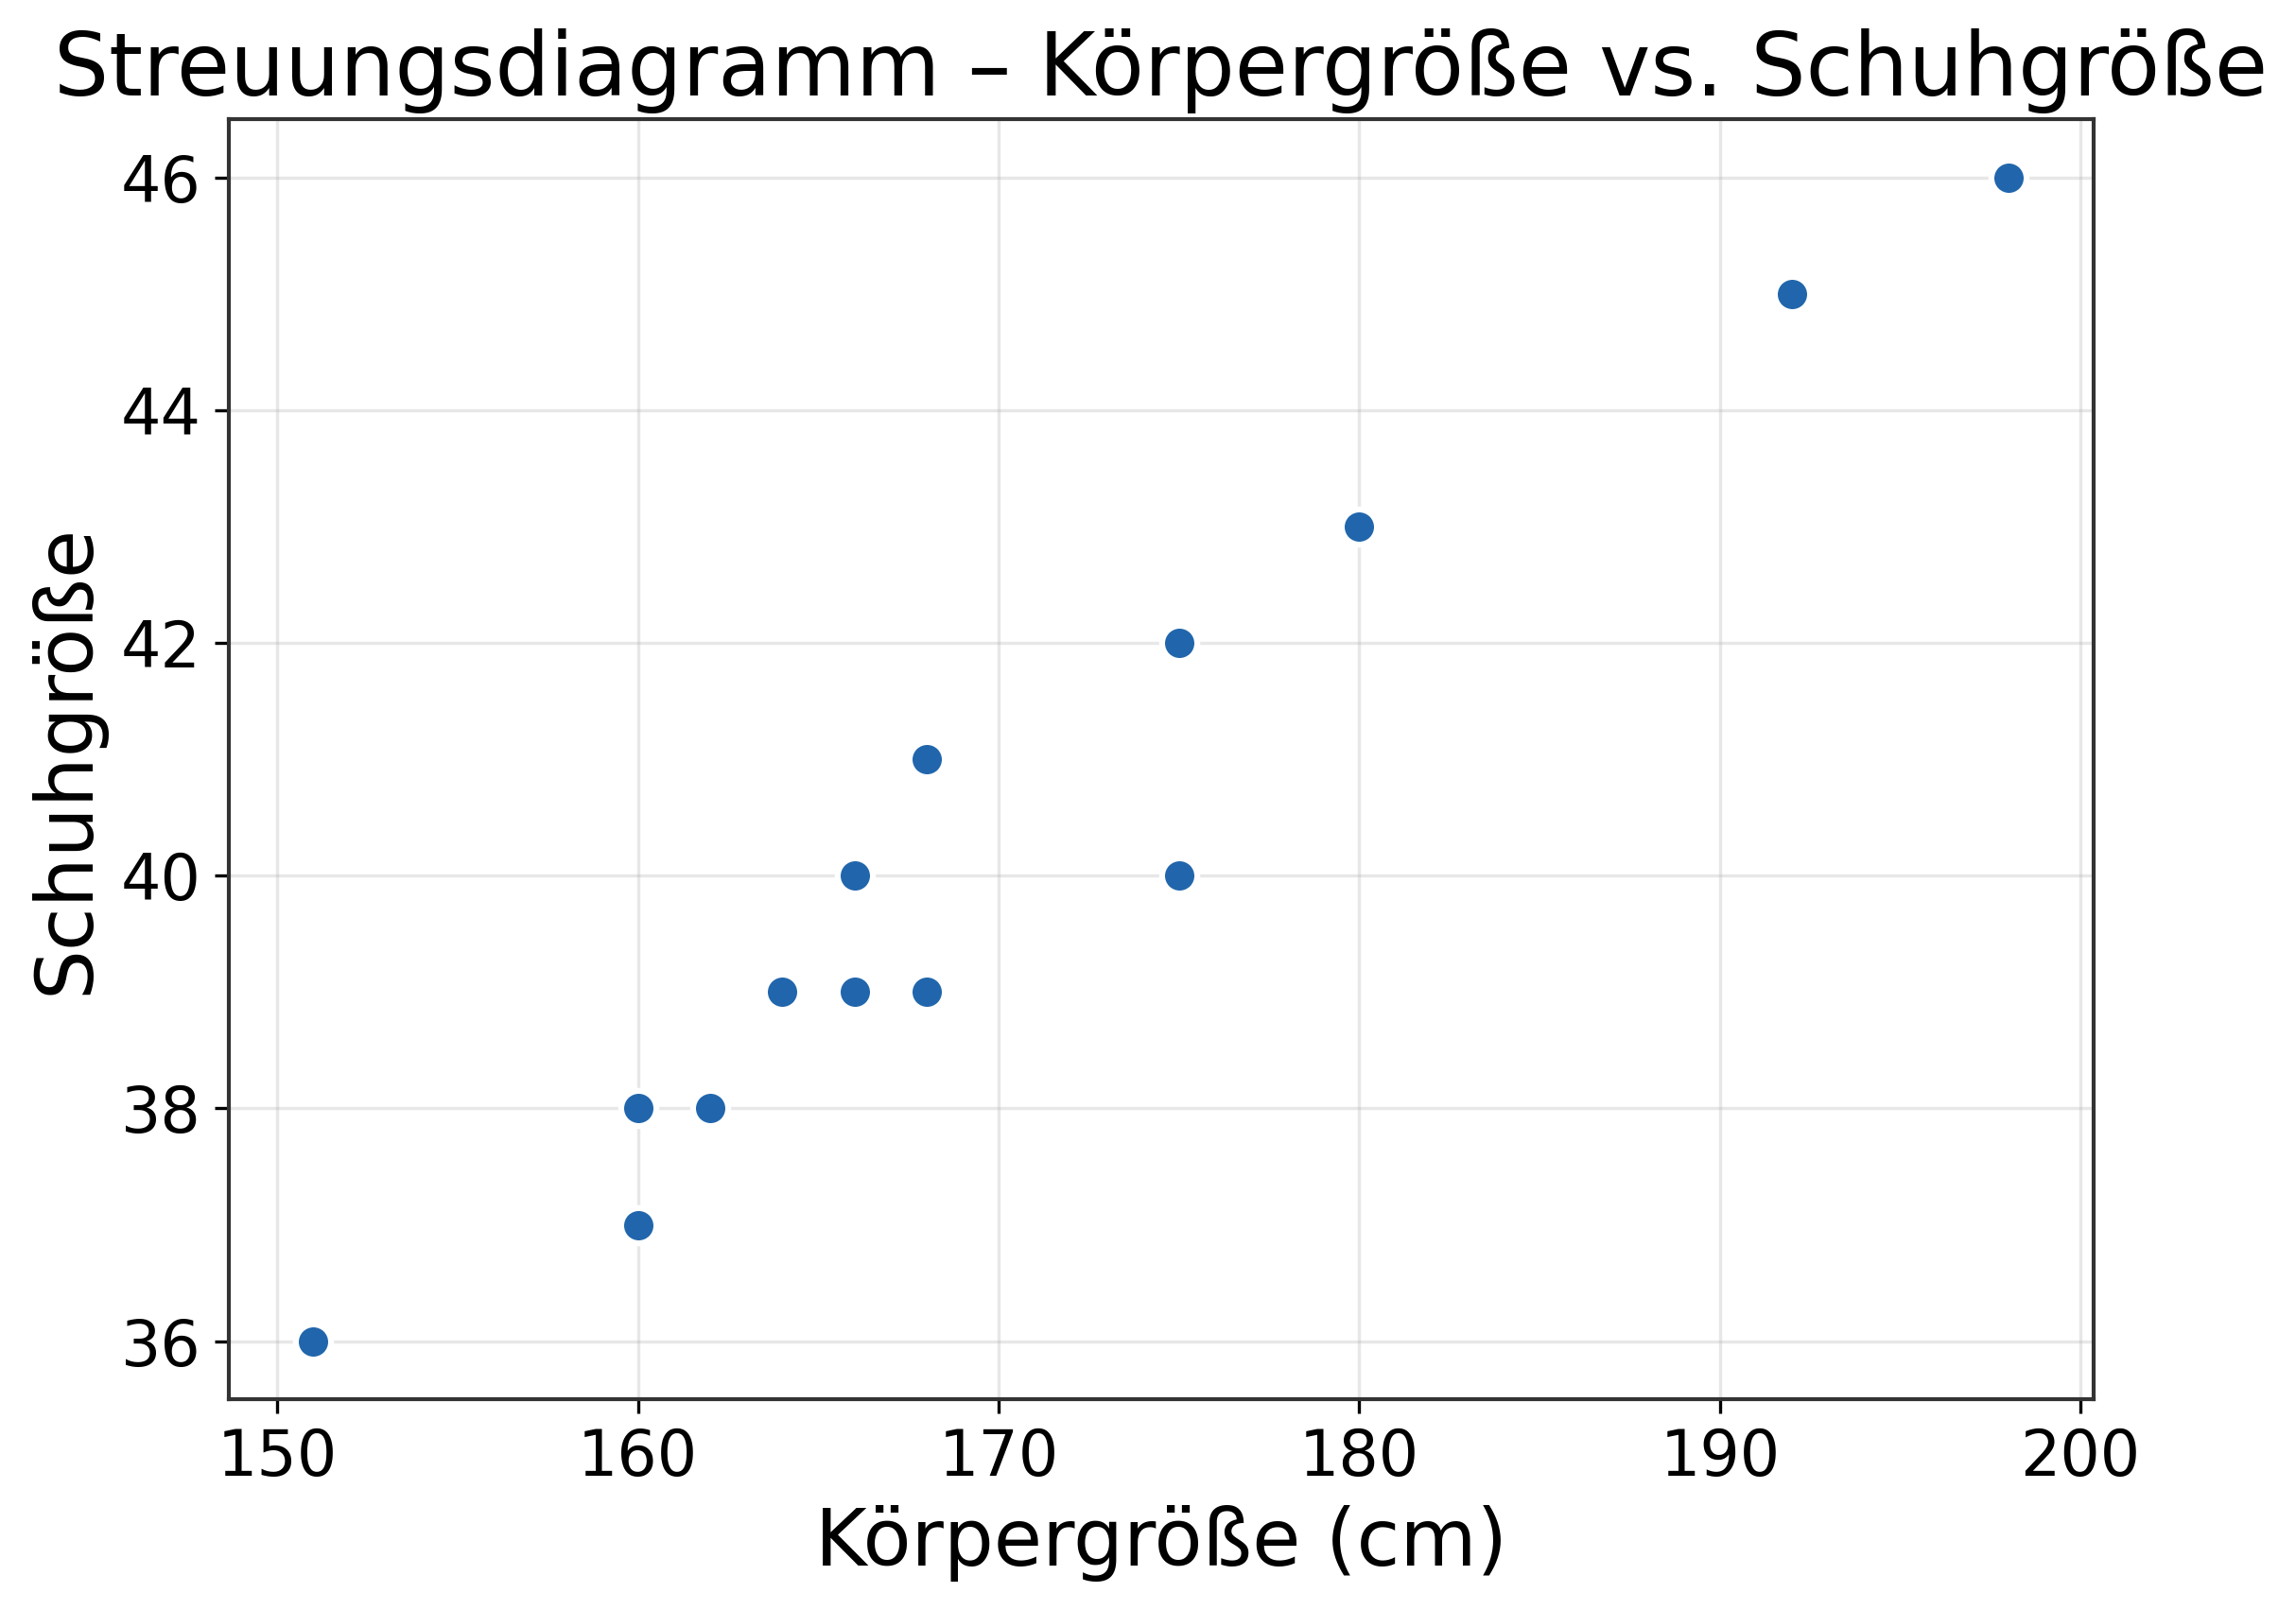
\includegraphics[width=0.85\textwidth,height=0.78\textheight,keepaspectratio]{images/image_026.png}
  \end{center}
\end{frame}

% ---- Slide 171: Streuungsdiagramm mit Regressionsgerade ----
\begin{frame}{{\large Übungsbeispiel Körpergrößen -- Schuhgrößen: Streuungsdiagramm mit Regressionsgerade}}
  \begin{center}
    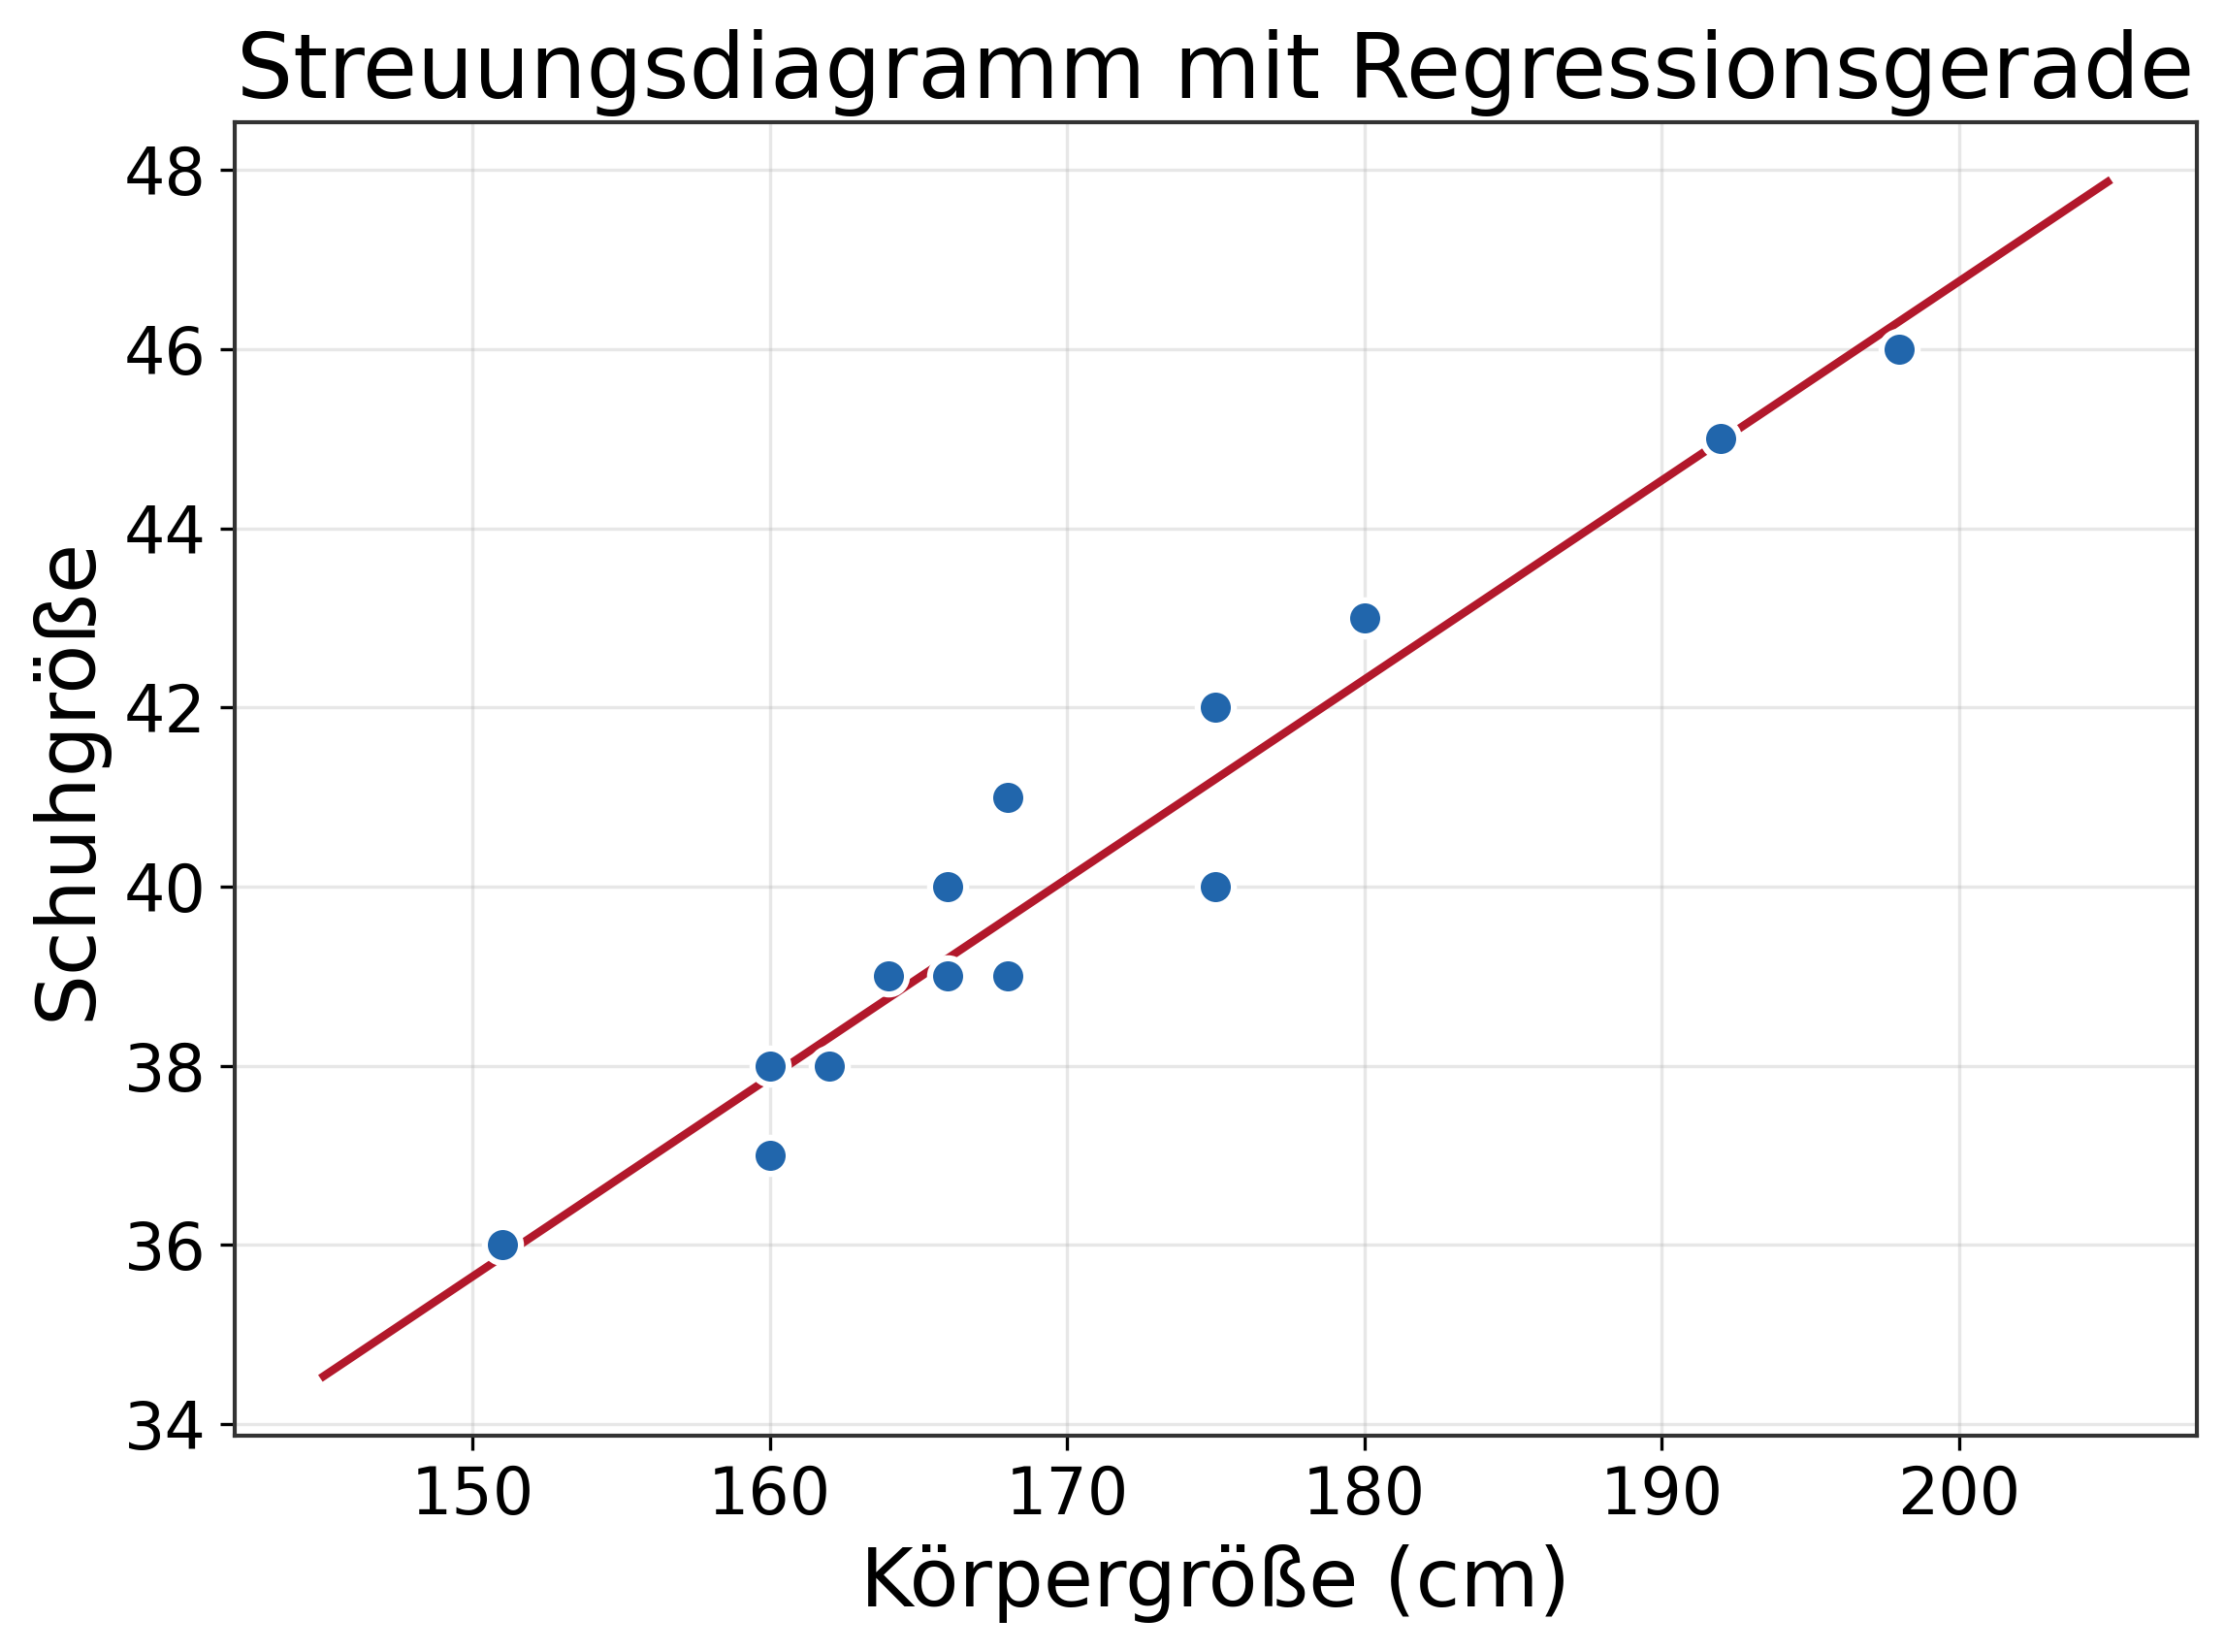
\includegraphics[width=0.85\textwidth,height=0.78\textheight,keepaspectratio]{images/image_027.png}
  \end{center}
\end{frame}

% ---- Slide 172: Residuenplot -------------------------------
\begin{frame}{Übungsbeispiel Körpergrößen -- Schuhgrößen: Residuenplot}
  \begin{center}
    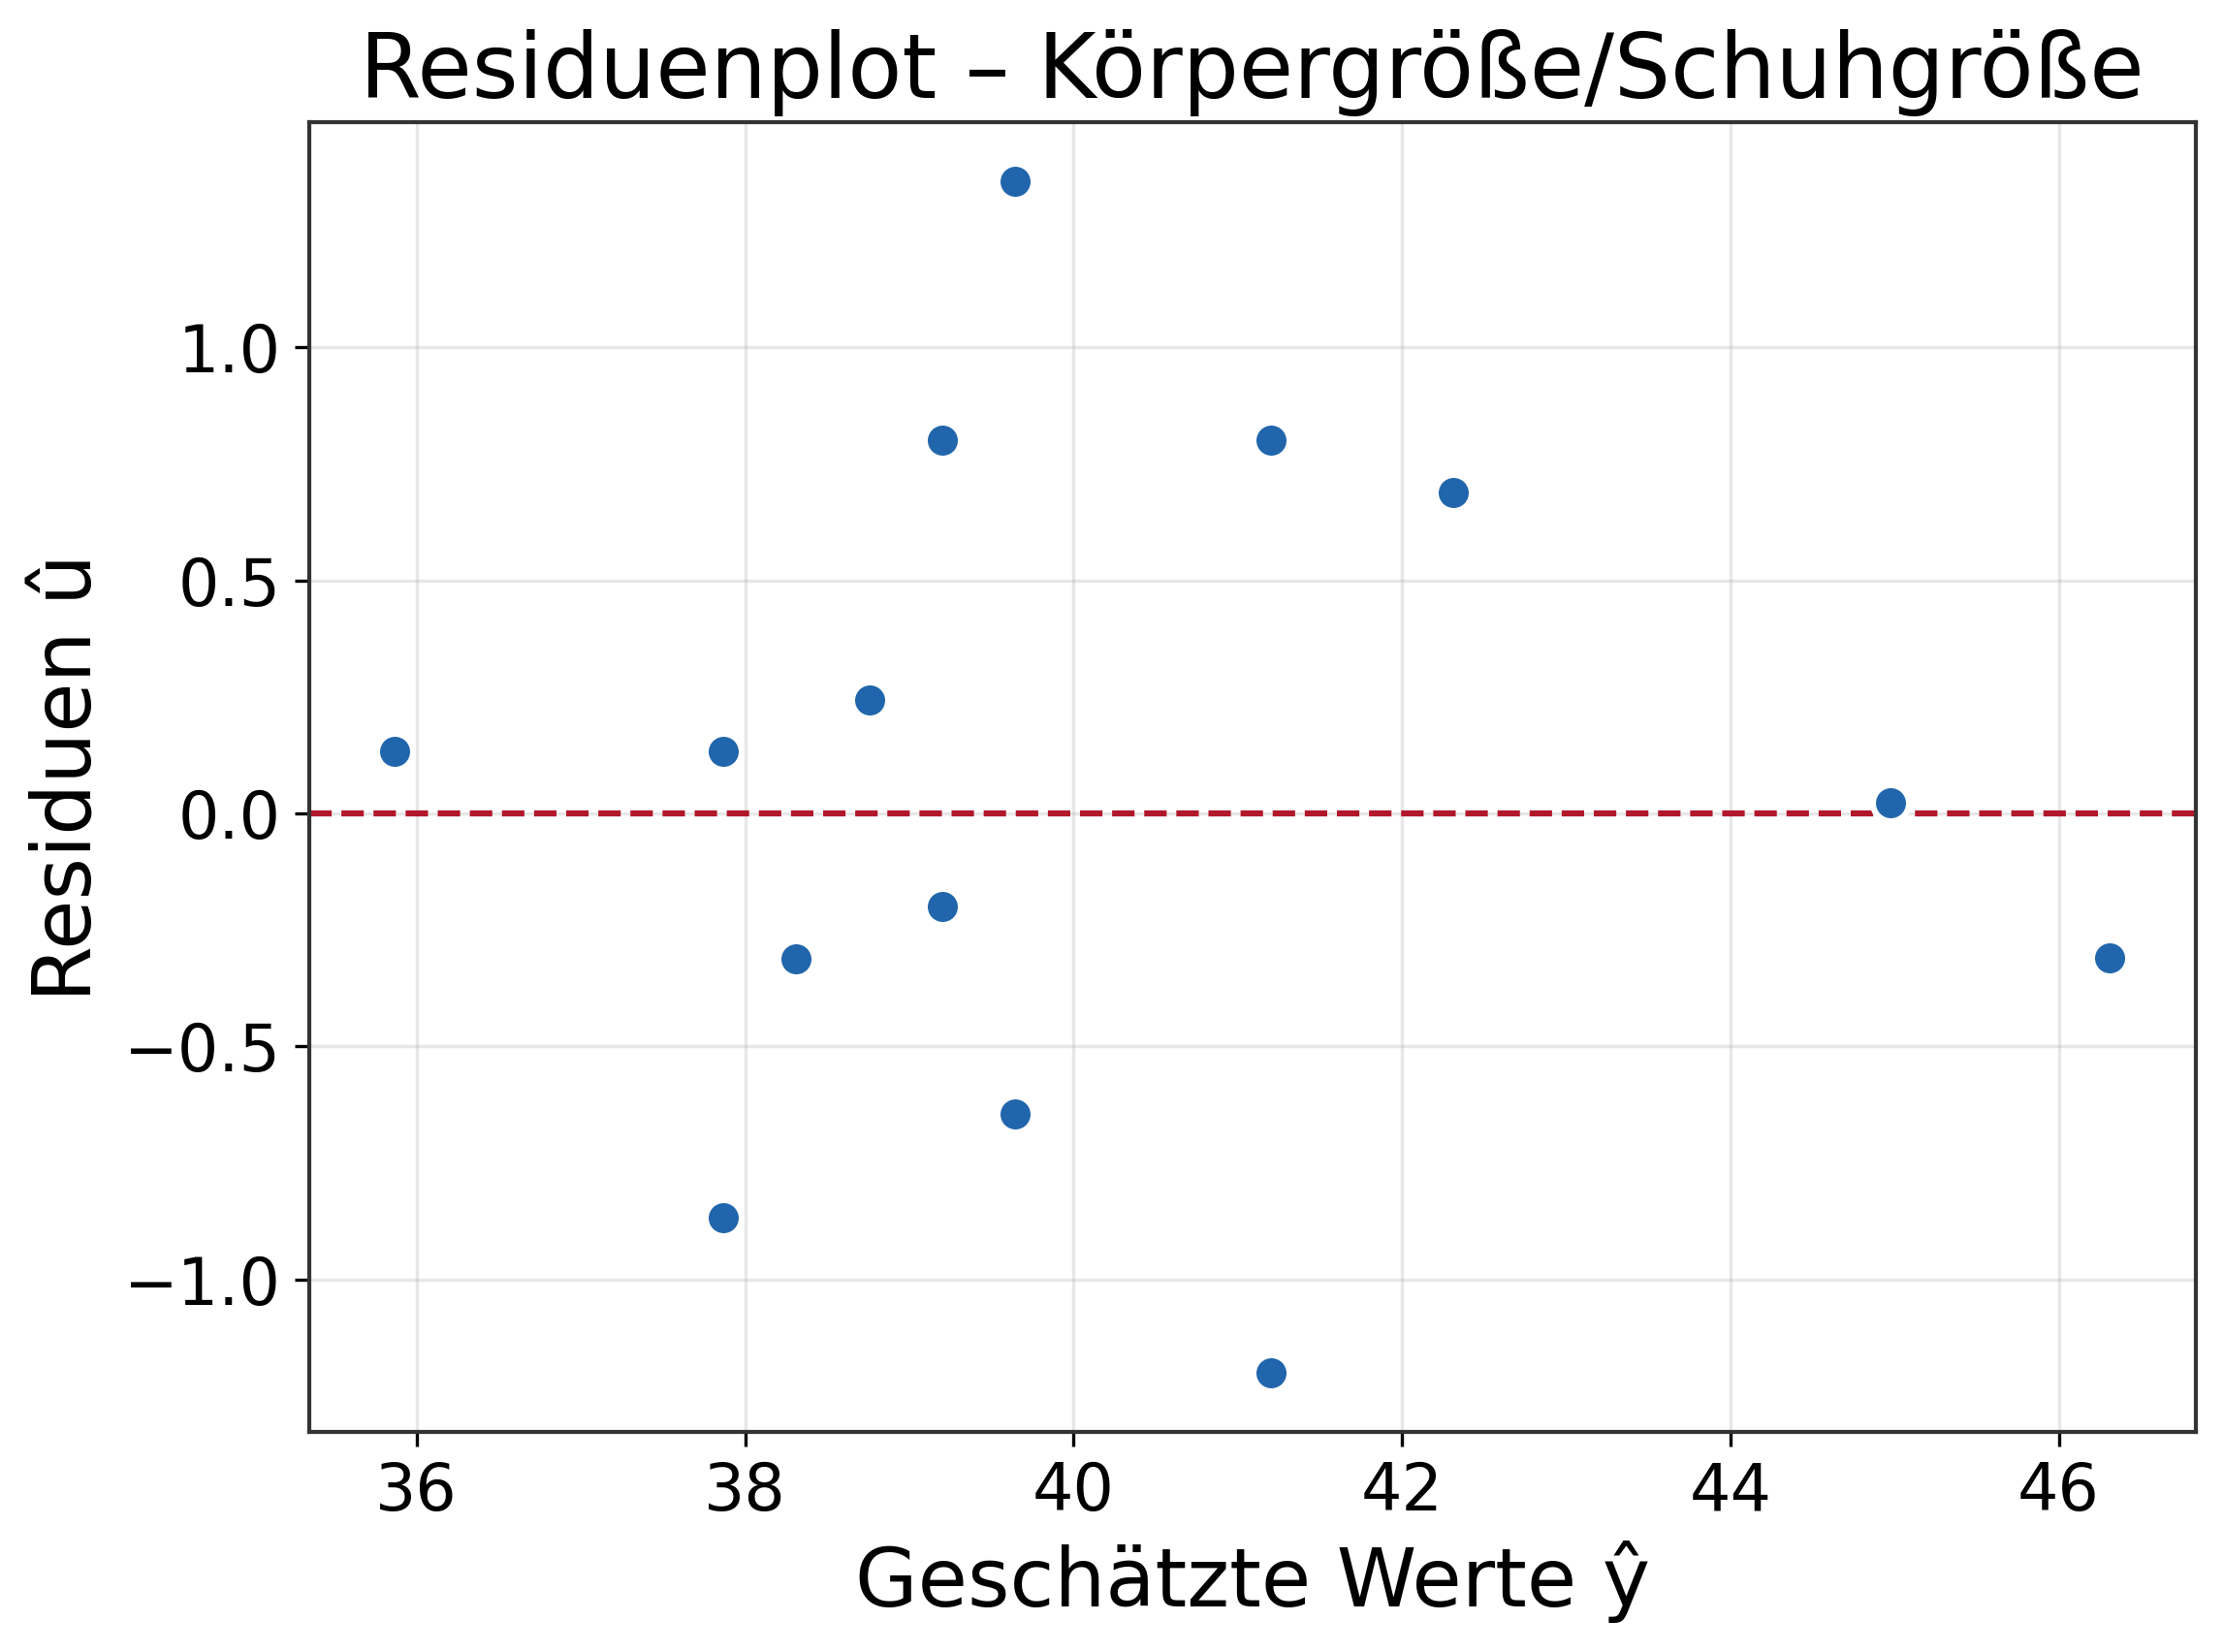
\includegraphics[width=0.85\textwidth,height=0.78\textheight,keepaspectratio]{images/image_028.png}
  \end{center}
\end{frame}

% ---- Slide 173: Residuenplot + Interpretation --------------
\begin{frame}{Übungsbeispiel Körpergrößen -- Schuhgrößen: Residuenplot}
  \begin{columns}[T]
    \begin{column}{0.62\textwidth}
      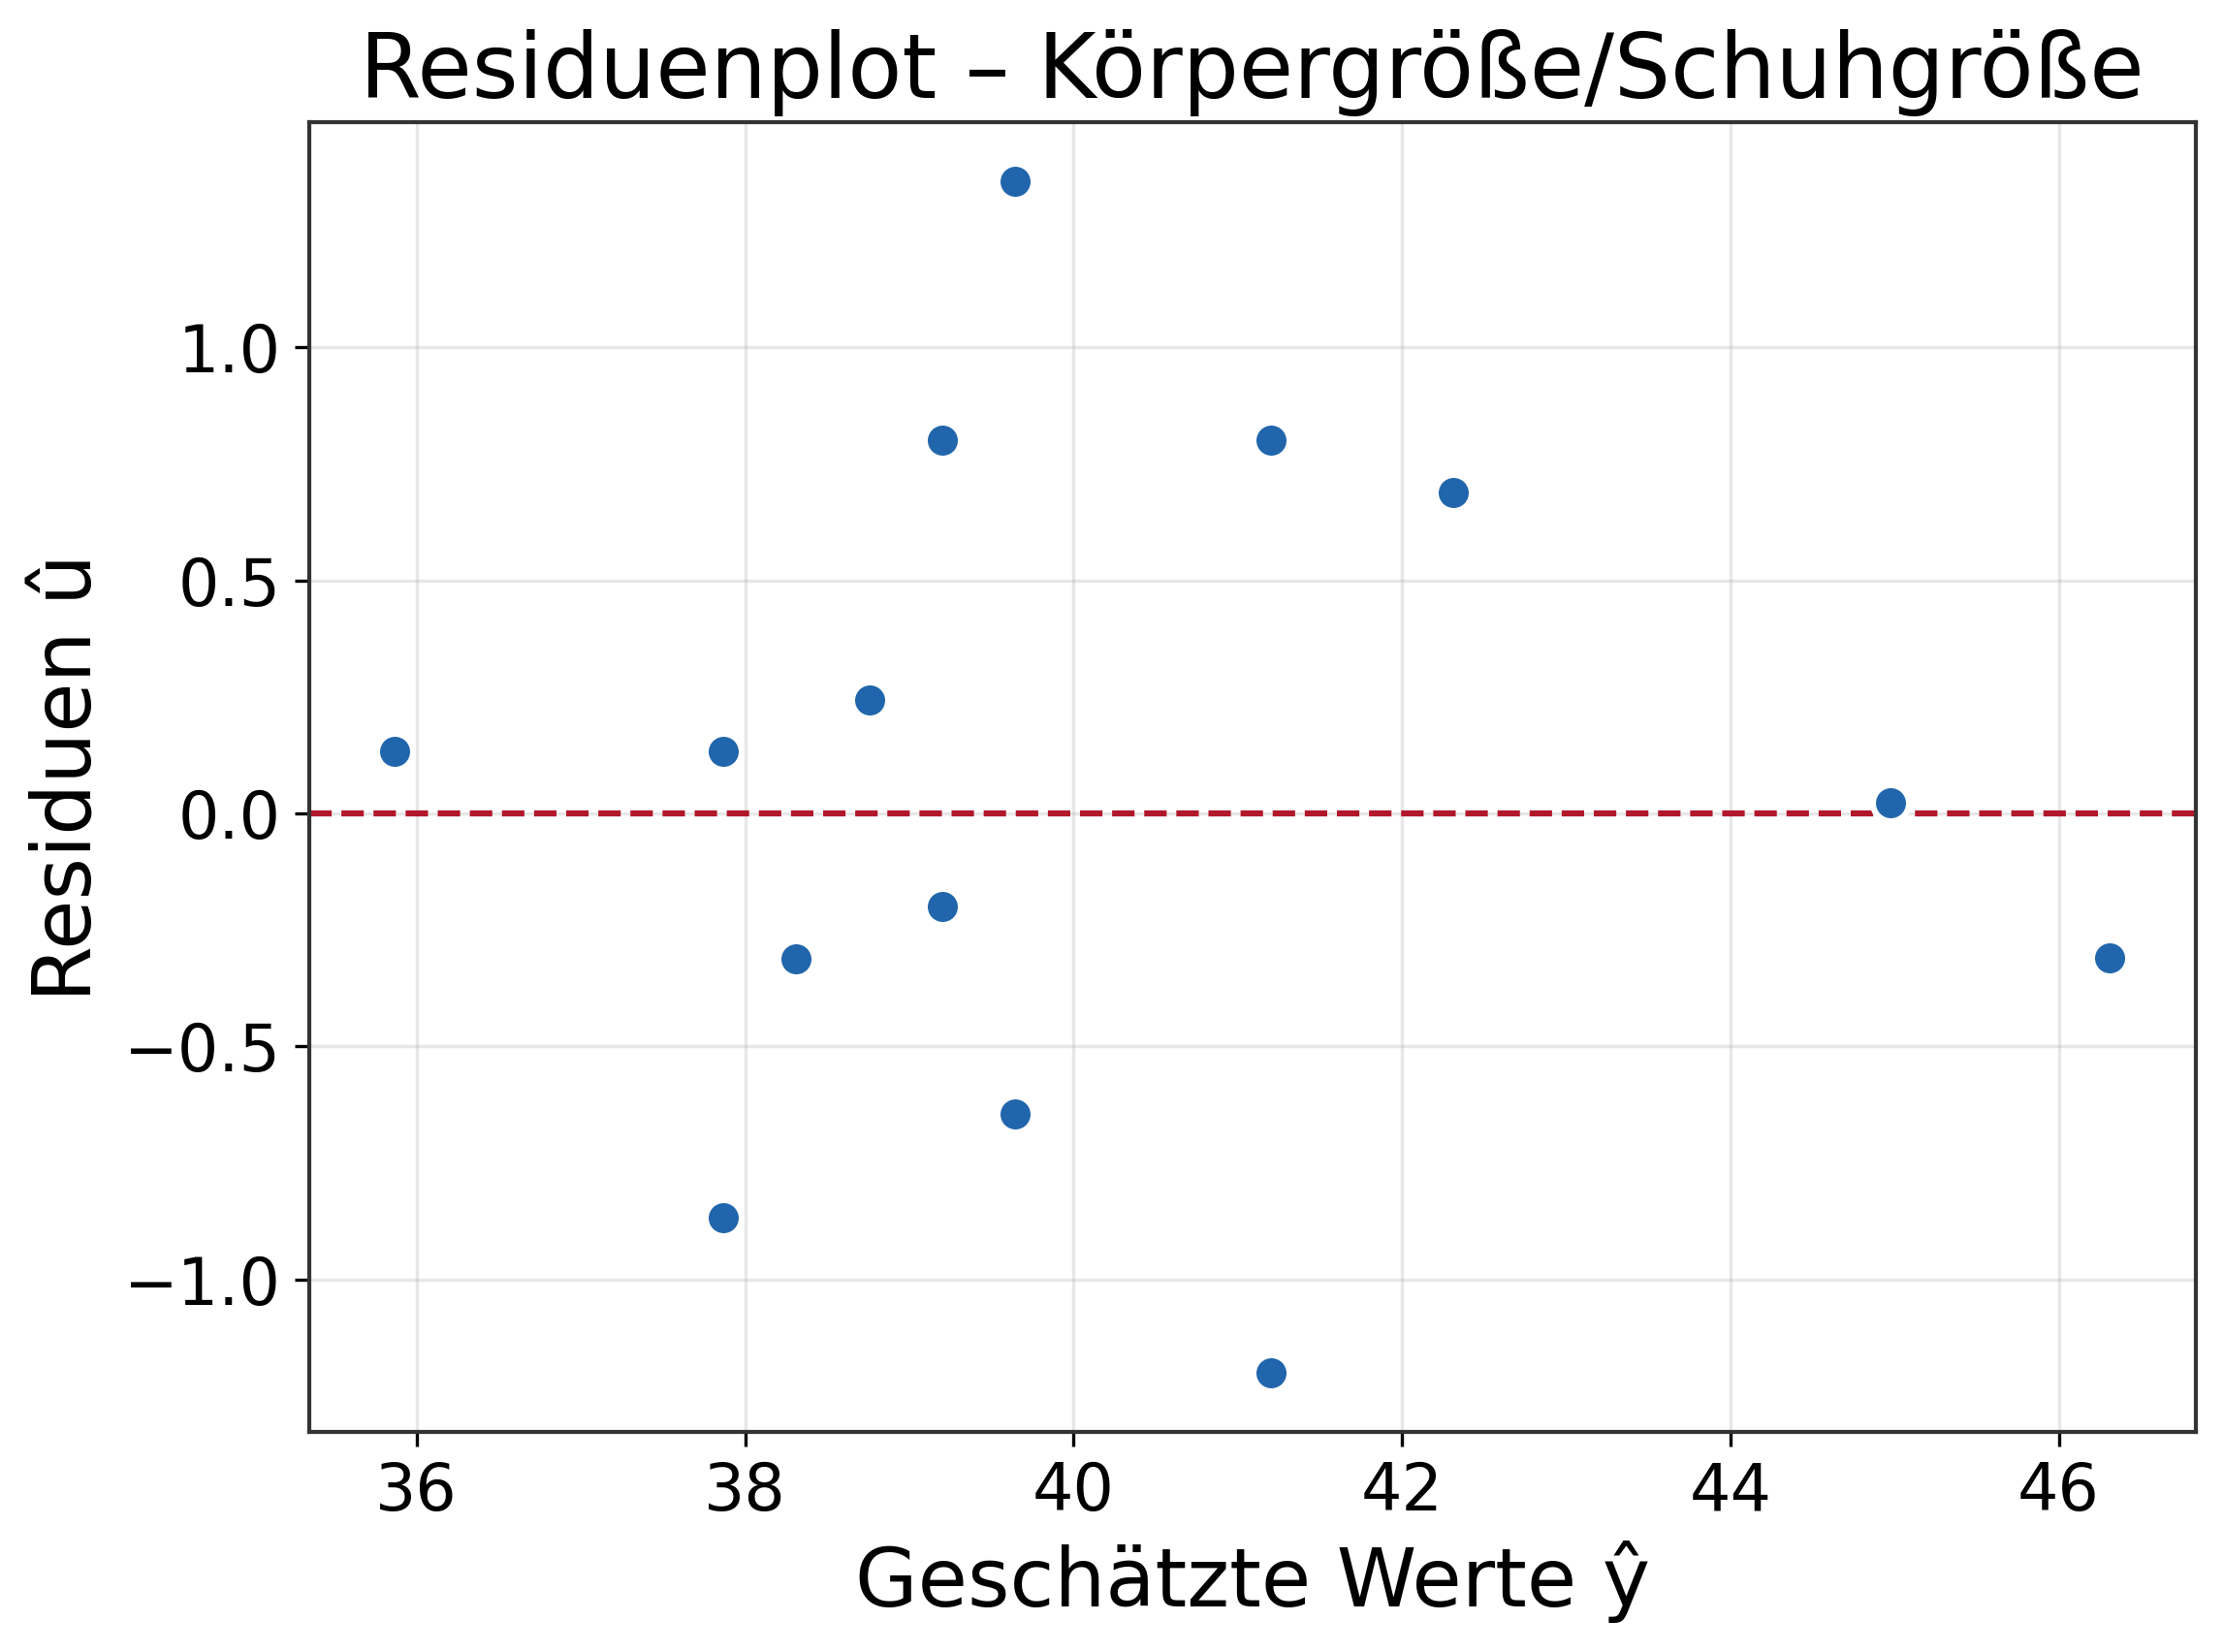
\includegraphics[width=\textwidth,height=0.78\textheight,keepaspectratio]{images/image_028.png}
    \end{column}
    \begin{column}{0.34\textwidth}
      \begin{exampleblock}{Beobachtung}
        \textbf{Keine Systematik erkennbar} \checkmark
      \end{exampleblock}
    \end{column}
  \end{columns}
\end{frame}

% ---- Slide 174: Übung QQ-Plot Aufgabe ----------------------
\begin{frame}{\spaceskip=0.27em plus 0.1em minus 0.05em\relax Übung QQ-Plot Körpergrößen -- Schuhgrößen: Residuen vs.\ Normalverteilung}% engere Wortabstände: Titel bleibt einzeilig
  \begin{block}{Aufgabe}
    Erstellen Sie einen QQ-Plot zwischen den Residuen aus dem
    Beispiel \emph{Körpergrößen -- Schuhgrößen} und der
    \textbf{Normalverteilung}.
  \end{block}
\end{frame}

% ---- Slide 174b: Lösung Aufgabe 3 -- Vorgehen QQ-Plot --------
\begin{frame}{Lösung Aufgabe 3 -- Vorgehen QQ-Plot}
  \begin{block}{Konstruktion des QQ-Plots}
    \begin{enumerate}
      \setlength{\itemsep}{0.25em}
      \item \textbf{Residuen} aus dem Modell berechnen:
            $\hat{u}_i = s_i - \hat{s}_i$ mit
            $\hat{s}_i = 2{,}3147 + 0{,}2222\,k_i$.
      \item Residuen \textbf{aufsteigend sortieren}:
            $\hat{u}_{(1)} \le \hat{u}_{(2)} \le \dots \le \hat{u}_{(n)}$.
      \item Theoretische Quantile der \textbf{Standardnormalverteilung}
            an den Stellen $p_i = \tfrac{i-0{,}5}{n}$ berechnen
            ($z_{(i)} = \Phi^{-1}(p_i)$).
      \item Punkte $\bigl(z_{(i)},\, \hat{u}_{(i)}\bigr)$ in ein
            Streuungsdiagramm eintragen.
    \end{enumerate}
  \end{block}

  \begin{exampleblock}{Beurteilungskriterium}
    Liegen die Punkte näherungsweise auf einer \textbf{Geraden},
    sind die Residuen \emph{normalverteilt} -- eine zentrale
    Annahme der linearen Regression.
  \end{exampleblock}
\end{frame}

% ---- Slide 175: QQ-Plot Ergebnis (Grafik) ------------------
\begin{frame}{\spaceskip=0.27em plus 0.1em minus 0.05em\relax Übung QQ-Plot Körpergrößen -- Schuhgrößen: Residuen vs.\ Normalverteilung}% engere Wortabstände: Titel bleibt einzeilig
  \begin{center}
    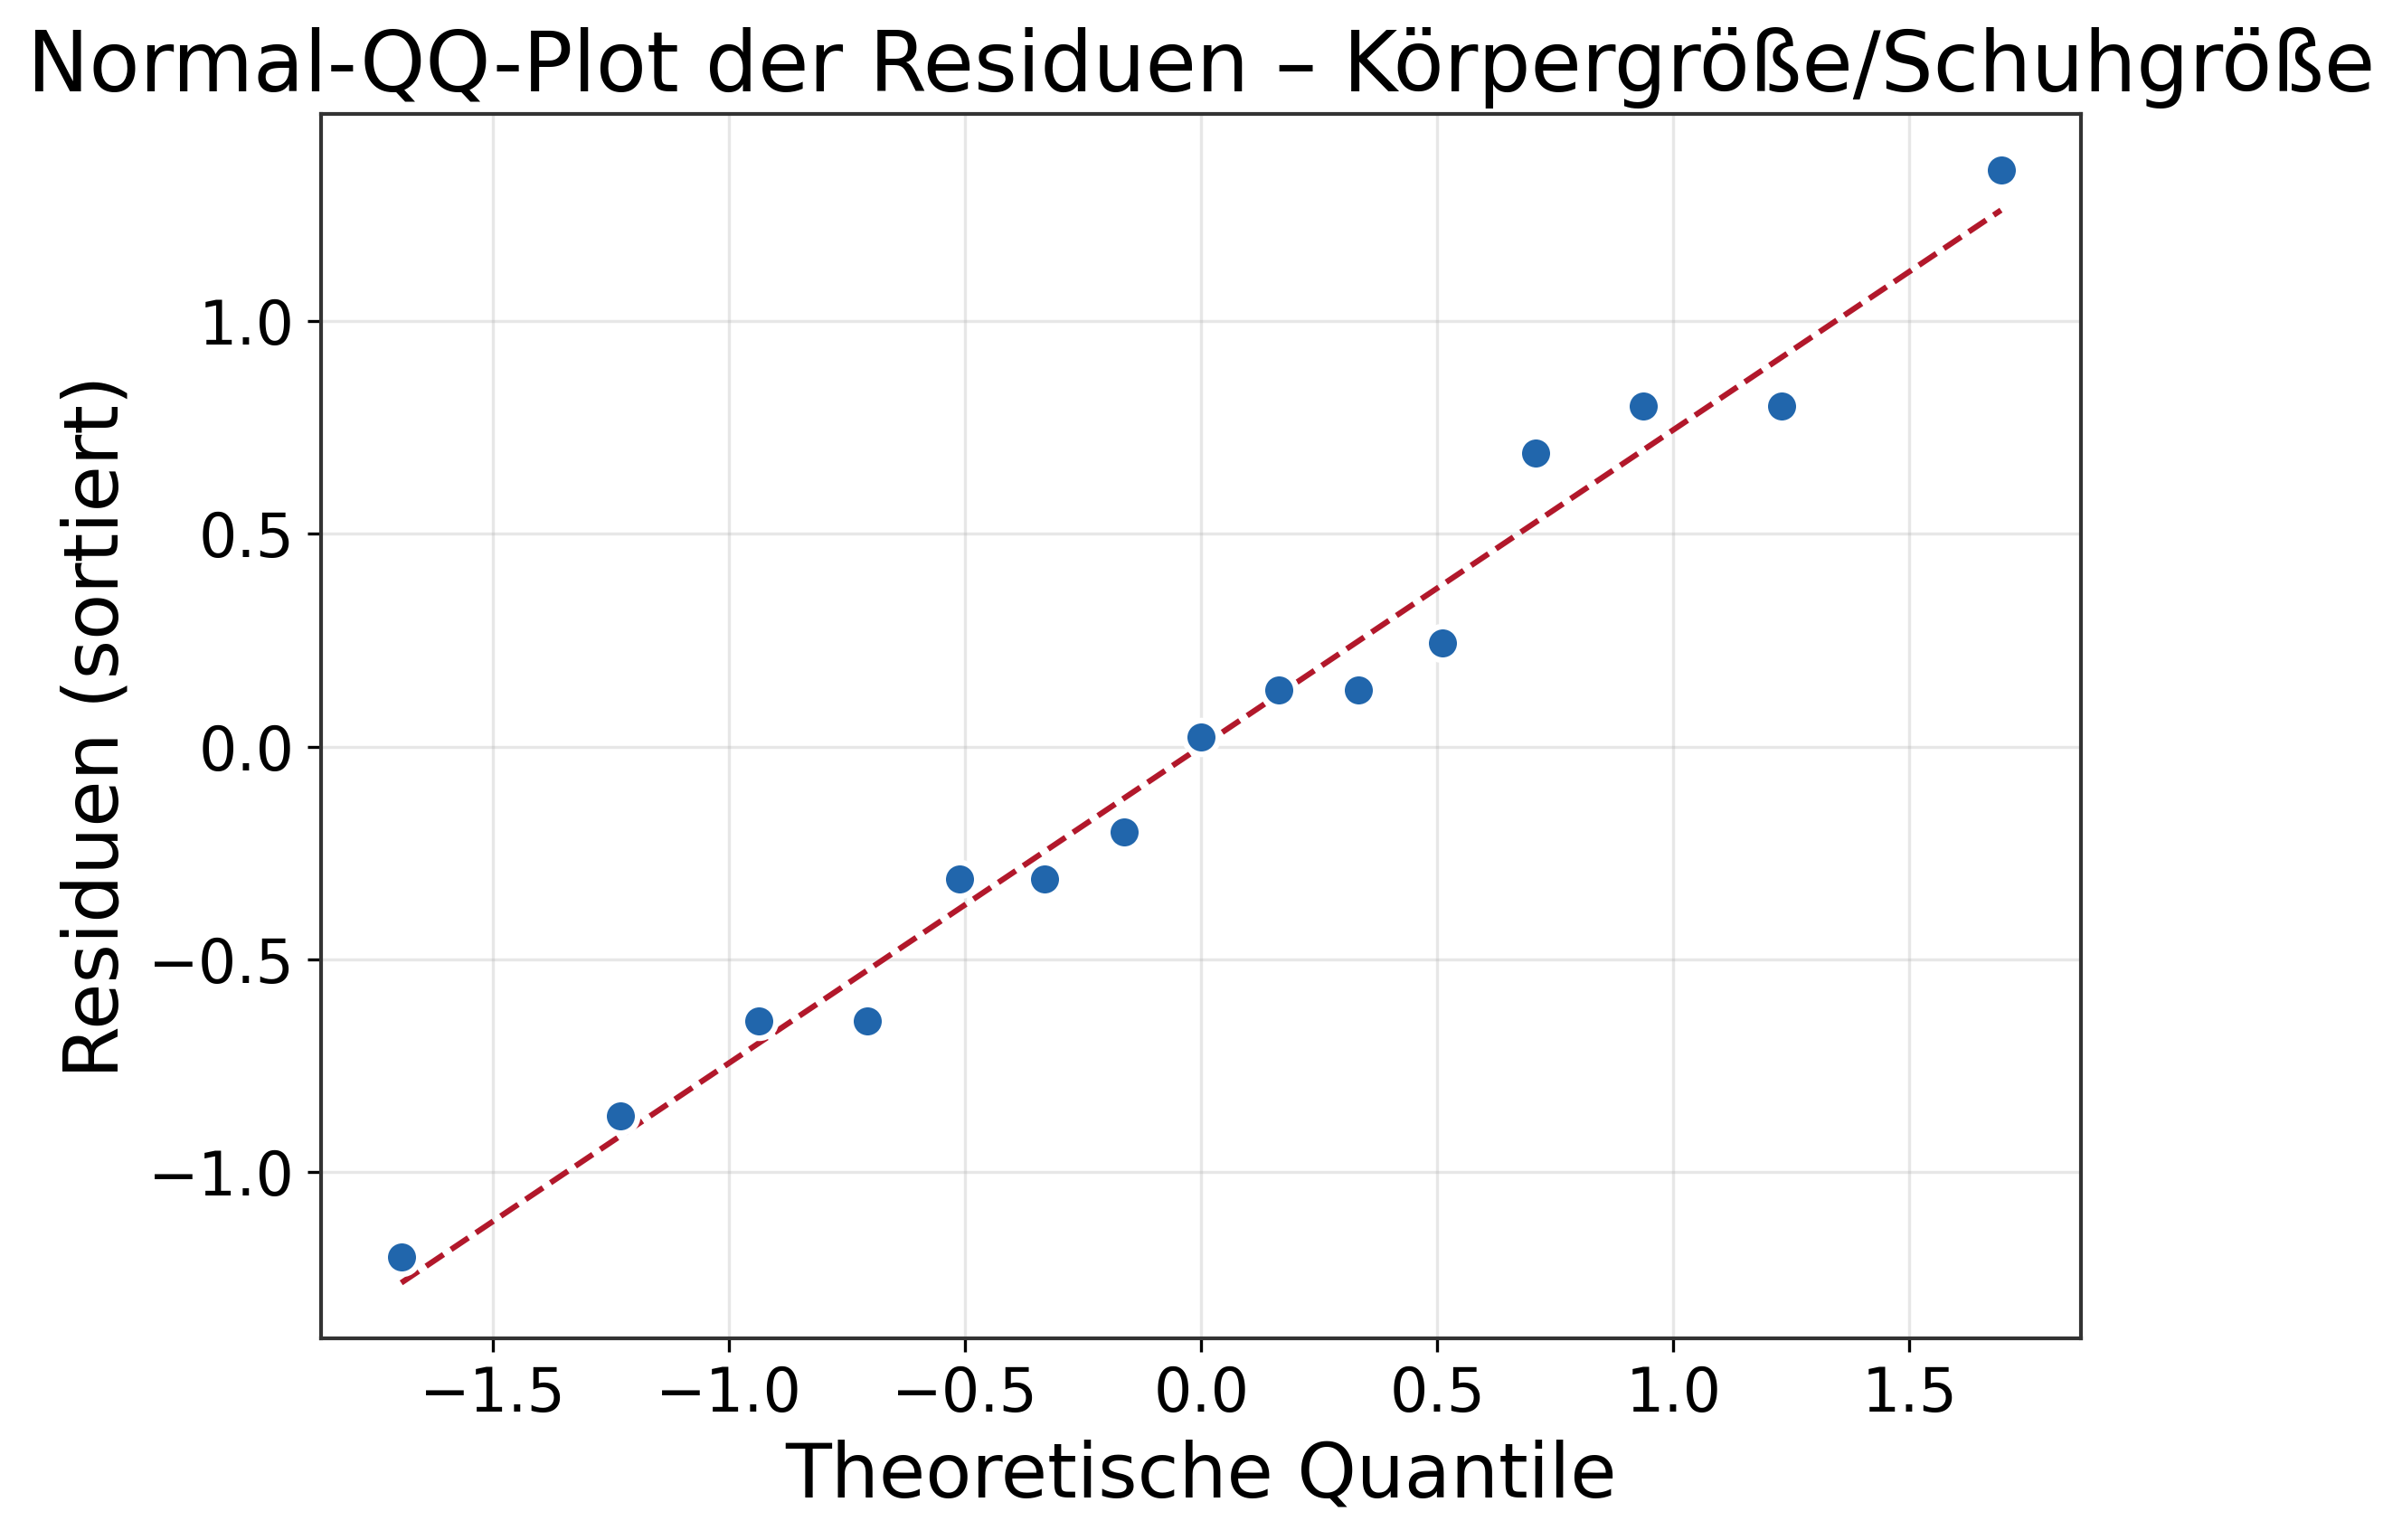
\includegraphics[width=0.85\textwidth,height=0.78\textheight,keepaspectratio]{images/image_029.png}
  \end{center}
\end{frame}

% ---- Slide 176: QQ-Plot Interpretation ---------------------
\begin{frame}{\spaceskip=0.27em plus 0.1em minus 0.05em\relax Übung QQ-Plot Körpergrößen -- Schuhgrößen: Residuen vs.\ Normalverteilung}% engere Wortabstände: Titel bleibt einzeilig
  \begin{columns}[T]
    \begin{column}{0.62\textwidth}
      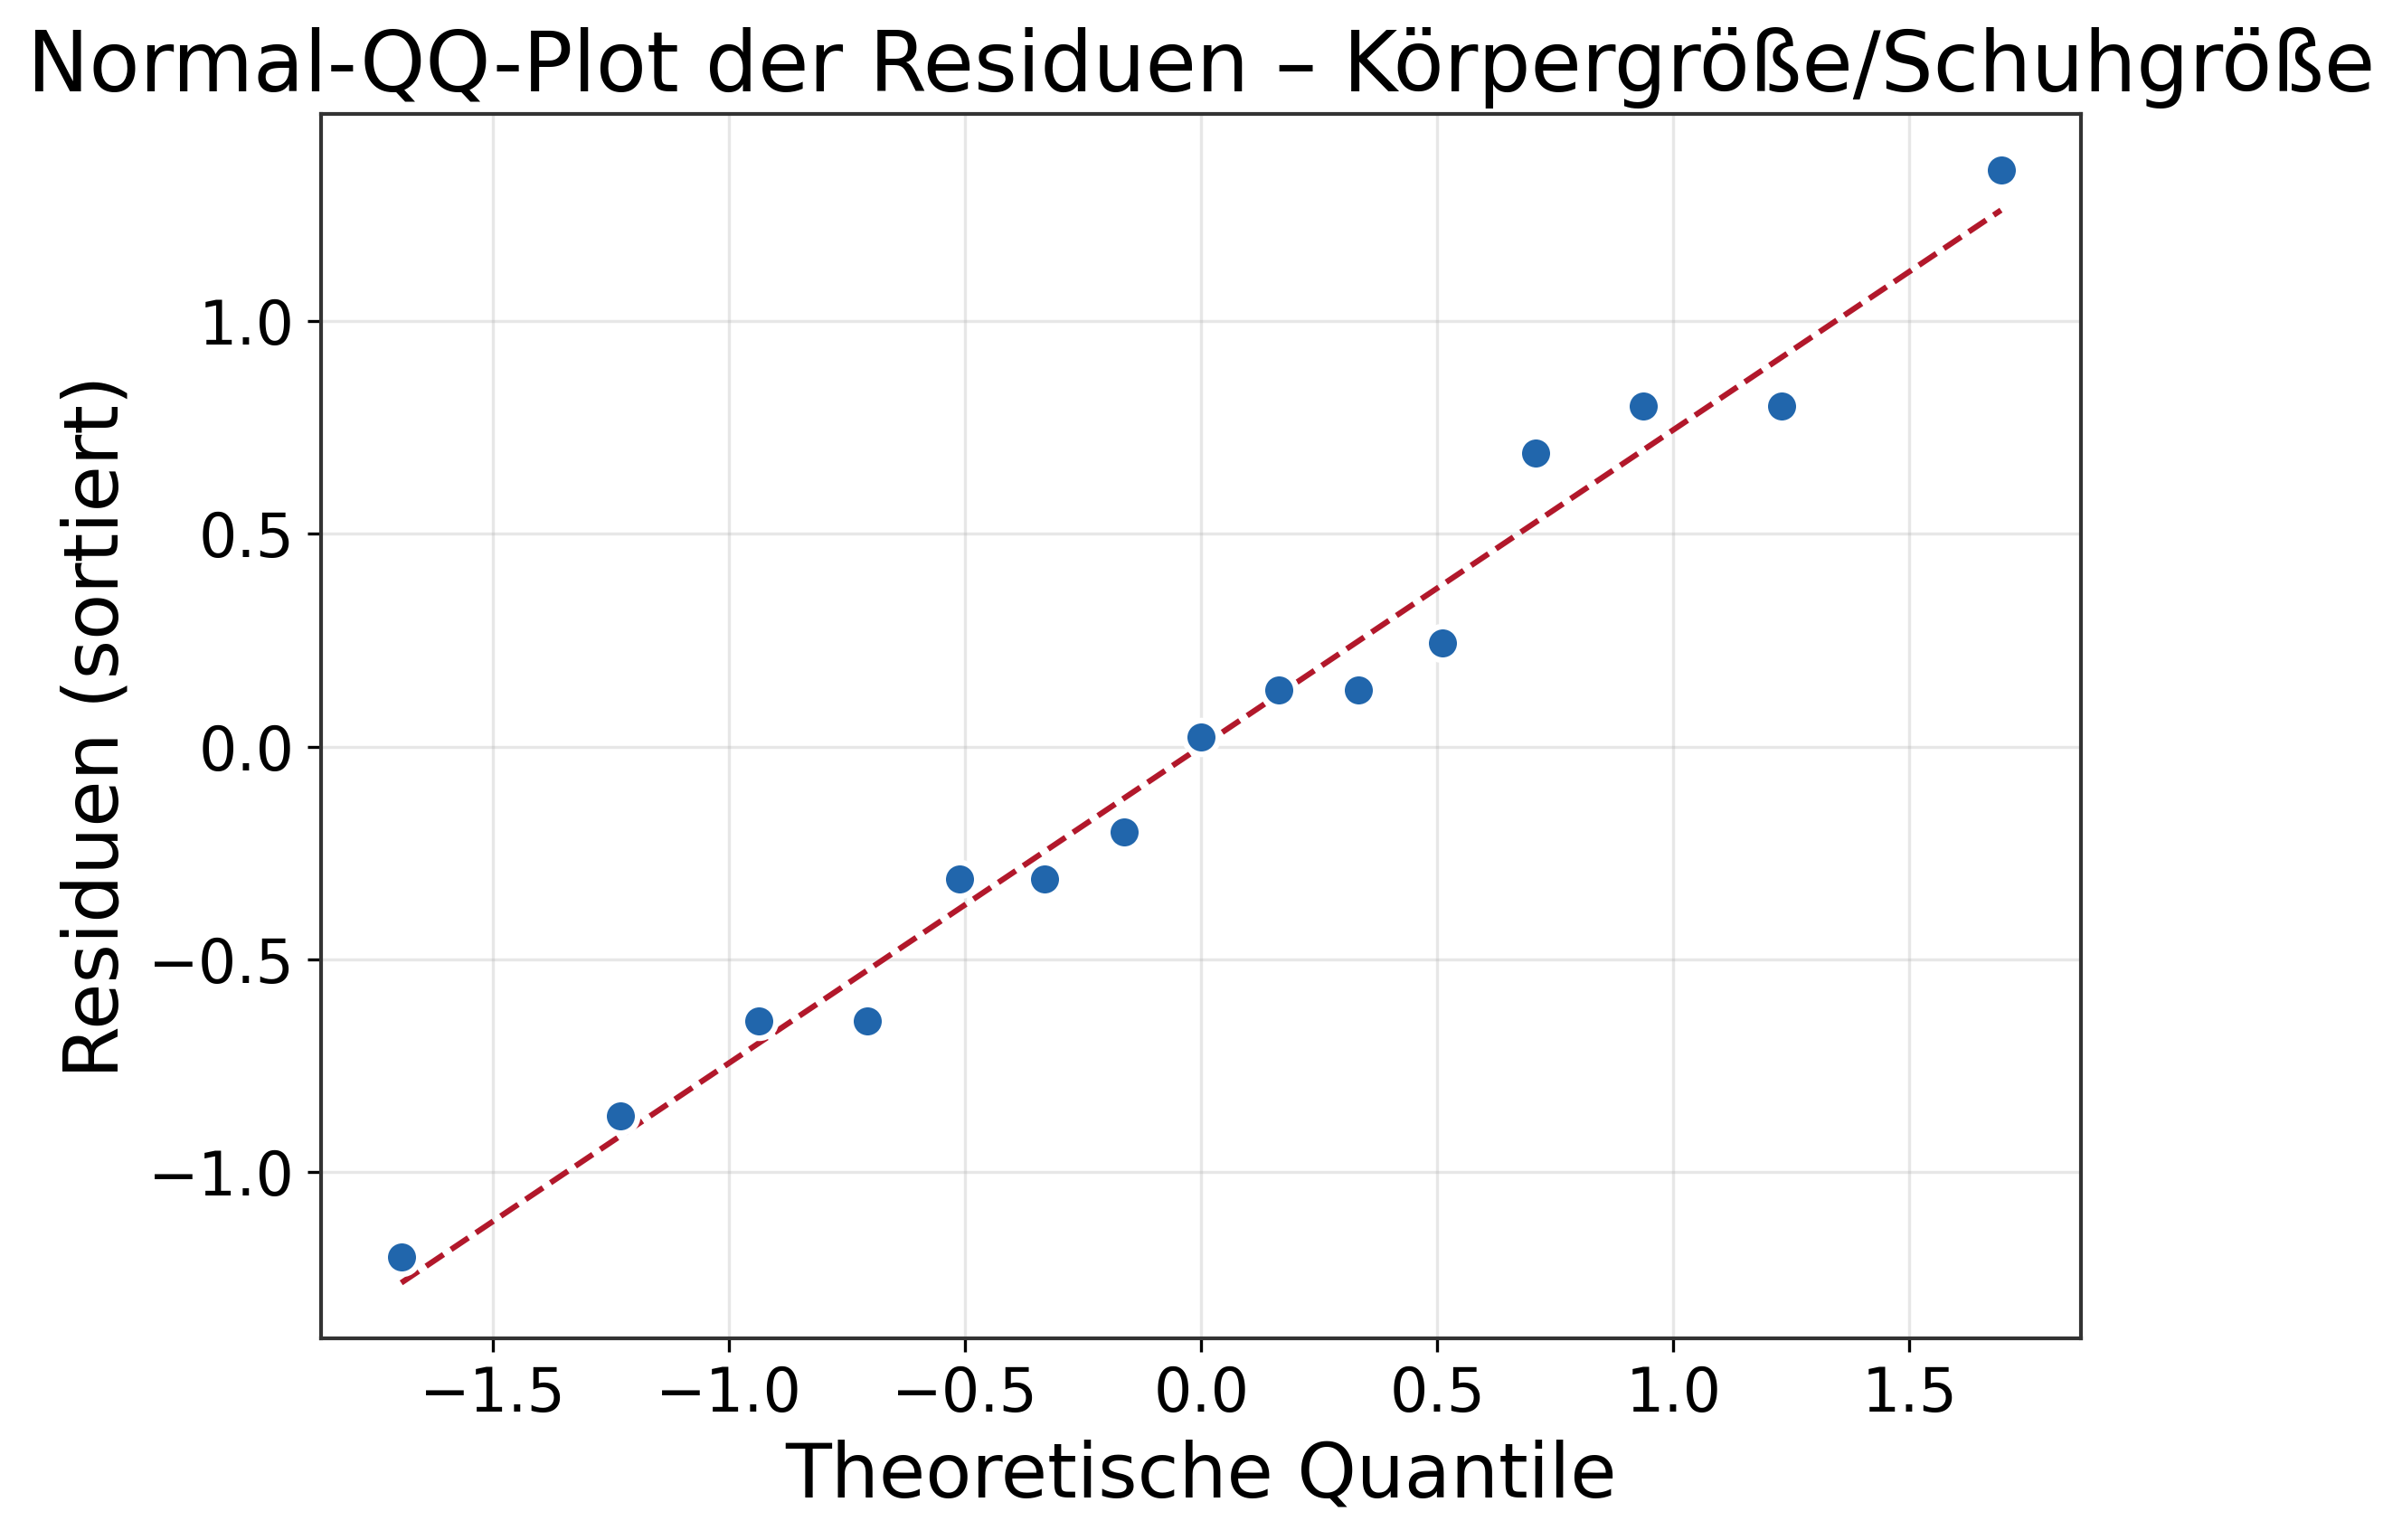
\includegraphics[width=\textwidth,height=0.78\textheight,keepaspectratio]{images/image_029.png}
    \end{column}
    \begin{column}{0.34\textwidth}
      \begin{exampleblock}{Fazit}
        \textbf{Erfüllt das Kriterium normalverteilt nahezu perfekt.}
      \end{exampleblock}
    \end{column}
  \end{columns}
\end{frame}

% ===== ZUSAMMENFASSUNGSFOLIEN TEIL 2 =====

\begin{frame}{Zusammenfassung 1: Grafische Darstellungen}
  \begin{center}
    \small
    \renewcommand{\arraystretch}{1.4}
    \begin{tabular}{l|>{\raggedright\arraybackslash}p{4.9cm}|>{\raggedright\arraybackslash}p{4.6cm}}
      \toprule
      \textbf{Methode} & \textbf{Beschreibung} & \textbf{Charakteristika} \\
      \midrule
      Emp.\ Verteilungsfkt. & Treppenfunktion der kum.\ Häufigkeiten & Sehr detailliert, aufwendig \\
      Histogramm & Säulendiagramm mit Dichte & Grober Überblick, klassenabhängig \\
      Boxplot & Quartile, Whisker, Ausreißer & Guter Überblick \\
      \bottomrule
    \end{tabular}
  \end{center}

  \begin{block}{Wichtige Formeln}
    \begin{description}
      \item[Dichte (Histogramm):] $\text{Dichte} = \frac{\text{relative Häufigkeit}}{\text{Klassenbreite}}$
      \item[Whisker-Min:] $\min\{x_i \mid x_i \geq Q_1 - 1{,}5 \cdot \text{IQR}\}$
      \item[Whisker-Max:] $\max\{x_i \mid x_i \leq Q_3 + 1{,}5 \cdot \text{IQR}\}$
    \end{description}
  \end{block}
\end{frame}

\begin{frame}{Zusammenfassung 2: Regression}
  \begin{block}{Regressionsmodell}
    \[ y_i = \beta_0 + \beta_1 x_i + u_i \qquad \hat{y}_i = \hat{\beta}_0 + \hat{\beta}_1 x_i \]
  \end{block}

  \begin{center}
    \renewcommand{\arraystretch}{1.4}
    \begin{tabular}{l|l}
      \toprule
      \textbf{Größe} & \textbf{Formel} \\
      \midrule
      Kovarianz & $s_{xy} = \frac{1}{n-1}\sum_{i=1}^{n}(x_i - \bar{x})(y_i - \bar{y})$ \\[4pt]
      Korrelationskoeffizient & $r_{xy} = \frac{s_{xy}}{s_x \cdot s_y} \qquad -1 \leq r_{xy} \leq 1$ \\[4pt]
      Steigung & $\hat{\beta}_1 = \frac{s_{xy}}{s_x^2}$ \\[4pt]
      Achsenabschnitt & $\hat{\beta}_0 = \bar{y} - \hat{\beta}_1 \bar{x}$ \\[4pt]
      Bestimmtheitsmaß & $R^2 = \frac{\text{ESS}}{\text{TSS}} = 1 - \frac{\text{RSS}}{\text{TSS}} = r_{xy}^2$ \\
      \bottomrule
    \end{tabular}
  \end{center}
\end{frame}

\begin{frame}{Zusammenfassung 3: Modelldiagnostik}
  \begin{block}{Residuen}
    \vspace{-0.3cm}
    \[ \hat{u}_i = y_i - \hat{y}_i \]
  \end{block}

  \vspace{0.2cm}

  \textbf{Residuenplot:} Keine Systematik $\to$ Modell ist angemessen
  \begin{itemize}
    \item Zu suchen: Trichterform, Kurven, Trends, Clustering
  \end{itemize}

  \vspace{0.3cm}

  \textbf{QQ-Plot:} Überprüfung der Normalverteilung der Residuen
  \begin{itemize}
    \item Ideal: Punkte liegen auf der Geraden
    \item Abweichungen an den Enden häufig und oft akzeptabel
    \item Systematische Muster deuten auf Nicht-Normalverteilung hin
  \end{itemize}

  \vspace{0.3cm}

  \textbf{Bestimmtheitsmaß -- Beurteilung:}
  \begin{center}
    \begin{tabular}{cccc}
      $R^2 > 0{,}9$: sehr gut & $0{,}7$--$0{,}9$: gut & $0{,}5$--$0{,}7$: mittel & $< 0{,}5$: schwach
    \end{tabular}
  \end{center}
\end{frame}

\begin{frame}[fragile]{Zusammenfassung: Wichtige R-Befehle (1/2)}
  \begin{block}{Grafische Darstellungen}
    \begin{lstlisting}
plot(ecdf(daten))                   # Empirische VF
hist(daten, freq = FALSE)           # Histogramm (Dichte)
hist(daten, breaks = c(37,39,41))   # Eigene Klassen
boxplot(daten)                      # Boxplot
\end{lstlisting}
  \end{block}

  \vspace{0.3cm}

  \begin{block}{Kovarianz und Korrelation}
    \begin{lstlisting}
cov(x, y)                          # Kovarianz
cor(x, y)                          # Korrelationskoeffizient
\end{lstlisting}
  \end{block}
\end{frame}

\begin{frame}[fragile]{Zusammenfassung: Wichtige R-Befehle (2/2)}
  \begin{block}{Regression}
    \begin{lstlisting}
reg <- lm(y ~ x)                    # Lineares Modell
summary(reg)                        # Ergebnisse inkl. R²
\end{lstlisting}
  \end{block}

  \vspace{0.3cm}

  \begin{block}{Modelldiagnostik}
    \begin{lstlisting}
plot(fitted(reg), resid(reg))       # Residuenplot
abline(h = 0, col = "red")          # Nulllinie
qqnorm(resid(reg))                  # QQ-Plot
qqline(resid(reg))                  # Referenzlinie
\end{lstlisting}
  \end{block}
\end{frame}

\end{document}
